\chapter{极性锑化铟的生长机理研究}
\section{引言}
III-V族化合物半导体被认为是下一代电子器件和光电子器件有利的材料候选。以III-V族化合物半导体\cemb{InSb}为例,块体状态的\cemb{InSb}具有较小的带隙和极高的电子迁移能力\citing{RN919-2019, RN897-1984, RN898-2020}。当结构尺度减小至低维,\cemb{InSb}展现出了更多新颖的物理特性,如非常强的自旋-轨道作用\citing{RN887-2021, RN922-2010, RN924-2015},较大的朗德g(Landé g-factor)因子\citing{RN925-2008}以及二维电子气等\citing{RN899-2020, RN926-2021}。这些新颖的物理特性使得低维\cemb{InSb}纳米结构可以用于自旋电子\citing{RN927-2017, RN928-2020},拓扑量子计算等量子器件的构建\citing{RN946-2017, RN737-2015, RN921-2016, RN933-2015}。同时,III-V族化合物半导体的单层化也有研究者进行了稳定性以及电子特性研究\citing{RN918-2013}。

在\ref{cap:石墨烯的生长机理研究}中,我们计算了石墨烯在化学气相沉积环境下的生长机理。以石墨烯为代表的单元素平面二维材料,在理想的晶格状态下所有原子都处于同一平面,具有平面外方向的镜面对称性和反演对称性\citing{RN664-2017, RN903-2021}。而对于晶格结构以闪锌矿(zinc blende,ZB)和纤锌矿(wurtzite,WZ)为主的III-V族化合物半导体,其晶格对称性决定了在<111>晶向缺少反演对称。反演对称性的破缺使得III-V族化合物半导体的(111)晶面具有两个不同的端面,即以III族元素为端点的III极性和以V族元素为端点的V极性。不同极性表面原子的不同导致了III-V化合物半导体不同极性的(111)面表现出不同的物理化学特性\citing{RN910-2004}。III-V化合物半导体的表面极性同时也对生长过程中的III-V化合物的生长机理以及生长形貌产生影响\citing{RN929-2015, RN916-2018}。先前的研究表明,\cemb{InSb(111)}表面的许多新奇的物理现象与所处的极性息息相关。例如在特定极性的\cemb{InSb(111)}表面可以异质外延生长具有优异电子性质的新型材料 \citing{RN902-2016, RN852-2021, RN901-2019, RN900-2017, RN891-2019}。

分子束外延(molecular beam epitaxy,MBE)技术以及各种高级材料观测技术(如球差矫正透射电子显微镜)的发展使得研究者能够进一步研究III-V化合物半导体生长过程中极性的演化及调控手段。1994年,研究者发现在\cemb{InSb/Sn/InSb}异质结构中,底端\cemb{InSb}的极性可以透过5原子层的\cemb{Sn}薄膜,对上层的\cemb{InSb}的极性产生影响。随后的研究发现,大多数的III-V化合物半导体倾向于生长V极性的纳米结构\citing{RN864-2019, RN930-1998, RN931-2010},通过不同的生长手段,也有研究者生长出了III极性的表面\citing{RN930-1998, RN931-2010}。通过对实验参数和生长环境进行细致的控制,研究者能够利用分子束外延的方法对所合成的III-V化合物半导体纳米结构进行生长极性控制 \citing{RN913-2016, RN858-2019, RN889-2011, RN911-2019}。得益于合成技术的发展,研究者对于III-V半导体的生长机制进行了大量的实验观测和理论探究,力图对其中的极性演化规律产生更深的理解,从而能够更好的对III-V化合物半导体低维纳米结构进行定极性生长\citing{RN878-2020, RN940-1979, RN936-2002, RN886-2021, RN932-2018, RN894-2012, RN934-2018, RN941-2016}。

在本章中,以III-V族化合物半导体\cemb{InSb}为例,我们系统的探究了双层\cemb{InSb(111)}在\cemb{Bi(001)}衬底上的生长序列以及形貌演化规律。我们的研究表明在\cemb{Bi}衬底上,\cemb{InSb}的极化从第二层生长开始。单层的\cemb{InSb}在在\cemb{Bi}衬底上表现出非晶的形态。我们绘制了双层\cemb{InSb}在
\cemb{Bi}衬底上的极化相图,并且探究了从单层到双层\cemb{InSb}表面极性变化的物理成因。
\section{计算细节}
在本章中,密度泛函理论主要使用Vienna ab-initio Simulation Package (VASP) 软件包进行计算\citing{RN681-1996, RN682-1996}。在密度泛函理论计算中,我们使用广义梯度近似(GGA)下的Perdew-Burke-Ernzerhof (PBE)泛函描述电子之间的交换关联作用\citing{RN683-1996}。平面波的截断动能取为为$\SI{500}{\electronvolt}$。\cemb{InSb(111)}与衬底\cemb{Bi(001)}之间的范德瓦尔斯作用使用Grimme的DFT-D3方法进行描述,并带有Becke-Johnson阻尼作用 \citing{RN937-2010, RN938-2011}。对于$1 \times 1$和$2 \times 2$大小的切片模型,我们使用以$\Gamma$ 点为中心的$11 \times 11 \times 1$和$7 \times 7 \times 1$的K空间采样网络进行布里渊区积分。而对于实空间体积更大的切片模型以及团簇模型,我们仅对$\Gamma$ 点进行采样。在原子结构优化的计算中,力收敛条件设为$\SI{1e-2}{\electronvolt \per \angstrom}$,电子结构自洽场计算的收敛条件设为$\SI{1e-6}{\electronvolt}$。对于过渡态的计算,我们采用CI-NEB(Climbing Image Nudged Elastic Band)方法对始末反应状态之间的能量鞍点进行搜寻,以确定反应势垒的大小\citing{RN790-2000}。对于过渡态计算,力收敛条件设为$\SI{3e-2}{\electronvolt \per \angstrom}$。

对于极性面的表面能,我们使用赝氢饱和法及四面体法进行计算\citing{RN300-2016}。用于表面能计算的\cemb{InSb}切片模型以及四面体模型均基于优化过的块体\cemb{InSb},并进行了进一步的结构优化。计算表面能的切片模型的大小为$2 \times 2$,包含至少9层\cemb{InSb(111)}双原子层。对于\cemb{InSb(111)/Bi(001)}体系,我们是由六层\cemb{Bi(001)}双原子层作为衬底。衬底底面原子在优化过程中固定在块体构型,用以模拟半无限衬底。在\cemb{Bi(001)}表面,\cemb{InSb(111)}覆盖层的晶格由于约$\SI{1.9}{\percent}$等晶格失配而有微小的形变。切片模型的垂直表面方向放置至少$\SI{20}{\angstrom}$的真空层以防止周期性条件相邻切片的影响。在我们的计算中,块体\cemb{InSb}和块体\cemb{Bi}的晶格常数分别为\SI{6.62}{\angstrom}和\SI{4.79}{\angstrom},与先前文献报道一致\citing{RN939-2013,RN1266-1965}。

为了估计原子之间的作用强弱,我们使用LOBSTER软件包对晶体轨道哈密顿量布居(Crystal Orbital Hamilton Population, COHP)进行了计算和分析\citing{RN951-2011, RN950-1993, RN949-2016}。在本章中,\cemb{InSb(111)/Bi(001)}体系中的成键强弱由-COHP谱和-COHP积分(-ICOHP)进行量化。-ICOHP由-COHP谱中的电子占据态积分而来。在-COHP和-ICOHP中,成键态以正值表示,反键态以负值表示。
\section{单层锑化铟的生长机理}

\subsection{\cemb{Bi(001)}衬底表面锑、铟原子的吸附机理}
\def\TfourSite{\rm T_{4} \it}
\def\HthreeSite{\rm H_{3} \it}
\def\mievpas{\milli\electronvolt\per\angstrom\squared}
\def\InSbMLpolar#1#2{\rm #1-In/#2-Sb}
\def\NumOfAdatom{\it N_{\rm adatoms} \it}
\def\CNinNsb#1#2#3#4{\rm #1/#2{}^{#3InV}_{#4SbT} \it}

对于\cemb{InSb(111)}极性面在\cemb{Bi(001)}衬底表面的生长机理,我们首先对衬底表面锑、铟原子的吸附进行研究。在衬底表面,吸附原子的结合能$\energyVar{b}{}$为\chinesecolon
\[
    \energyVar{b}{}=\left(\energyVar{sub+adatom}{}-\energyVar{sub}{}-N\muVar{adatom}{}\right)/ N
\]

其中,$\energyVar{sub+adatom}{}$和$\energyVar{sub}{}$为吸附有原子的衬底和未吸附原子的衬底的能量。$\muVar{adatom}{}$为吸附原子的化学势。$N$为吸附原子的总数。

我们考虑\cemb{In}和\cemb{Sb}吸附原子在\cemb{Bi(001)}表面吸附覆盖率为$1/ 4$的结合能,计算结果如\ref{fig:IS_Bi_adatoms}所示。根据我们的计算,\cemb{In}原子和\cemb{Sb}原子都更倾向于吸附在\cemb{Bi(001)}衬底表面的$\TfourSite$位和$\HthreeSite$位。如图\ref{fig:IS_structure_T4onBi}和\ref{fig:IS_structure_H3onBi}所示,$\TfourSite$为\cemb{Bi(001)}衬底表面的四重配位顶位,正对于第一层\cemb{Bi}双原子层的下层原子。$HthreeSite$为\cemb{Bi(001)}衬底表面的三种配位空心位,正对于第一层\cemb{Bi}双原子层的空心以及第二层\cemb{Bi}双原子层的上层原子。\cemb{In}原子和\cemb{Sb}原子在\cemb{Bi(001)}衬底表面的吸附能如图\ref{fig:IS_DFT_adatomBind}所示,计算表明\cemb{Bi(001)}衬底表面的$\TfourSite$为\cemb{In}原子和\cemb{Sb}原子的最佳吸附位点。而$\HthreeSite$为二者的次优吸附位点。在吸附能以及后续的能量计算中,我们使用\cemb{In}的化学势$\muVar{In}{}$来表示\cemb{In}元素在生长气氛中的活性水平,体现在\cemb{InSb}化学平衡下\cemb{In}元素和\cemb{Sb}元素的浓度差距。

\begin{figure}[htb]
    \subfloat[]{
        \label{fig:IS_DFT_adatomBind}
        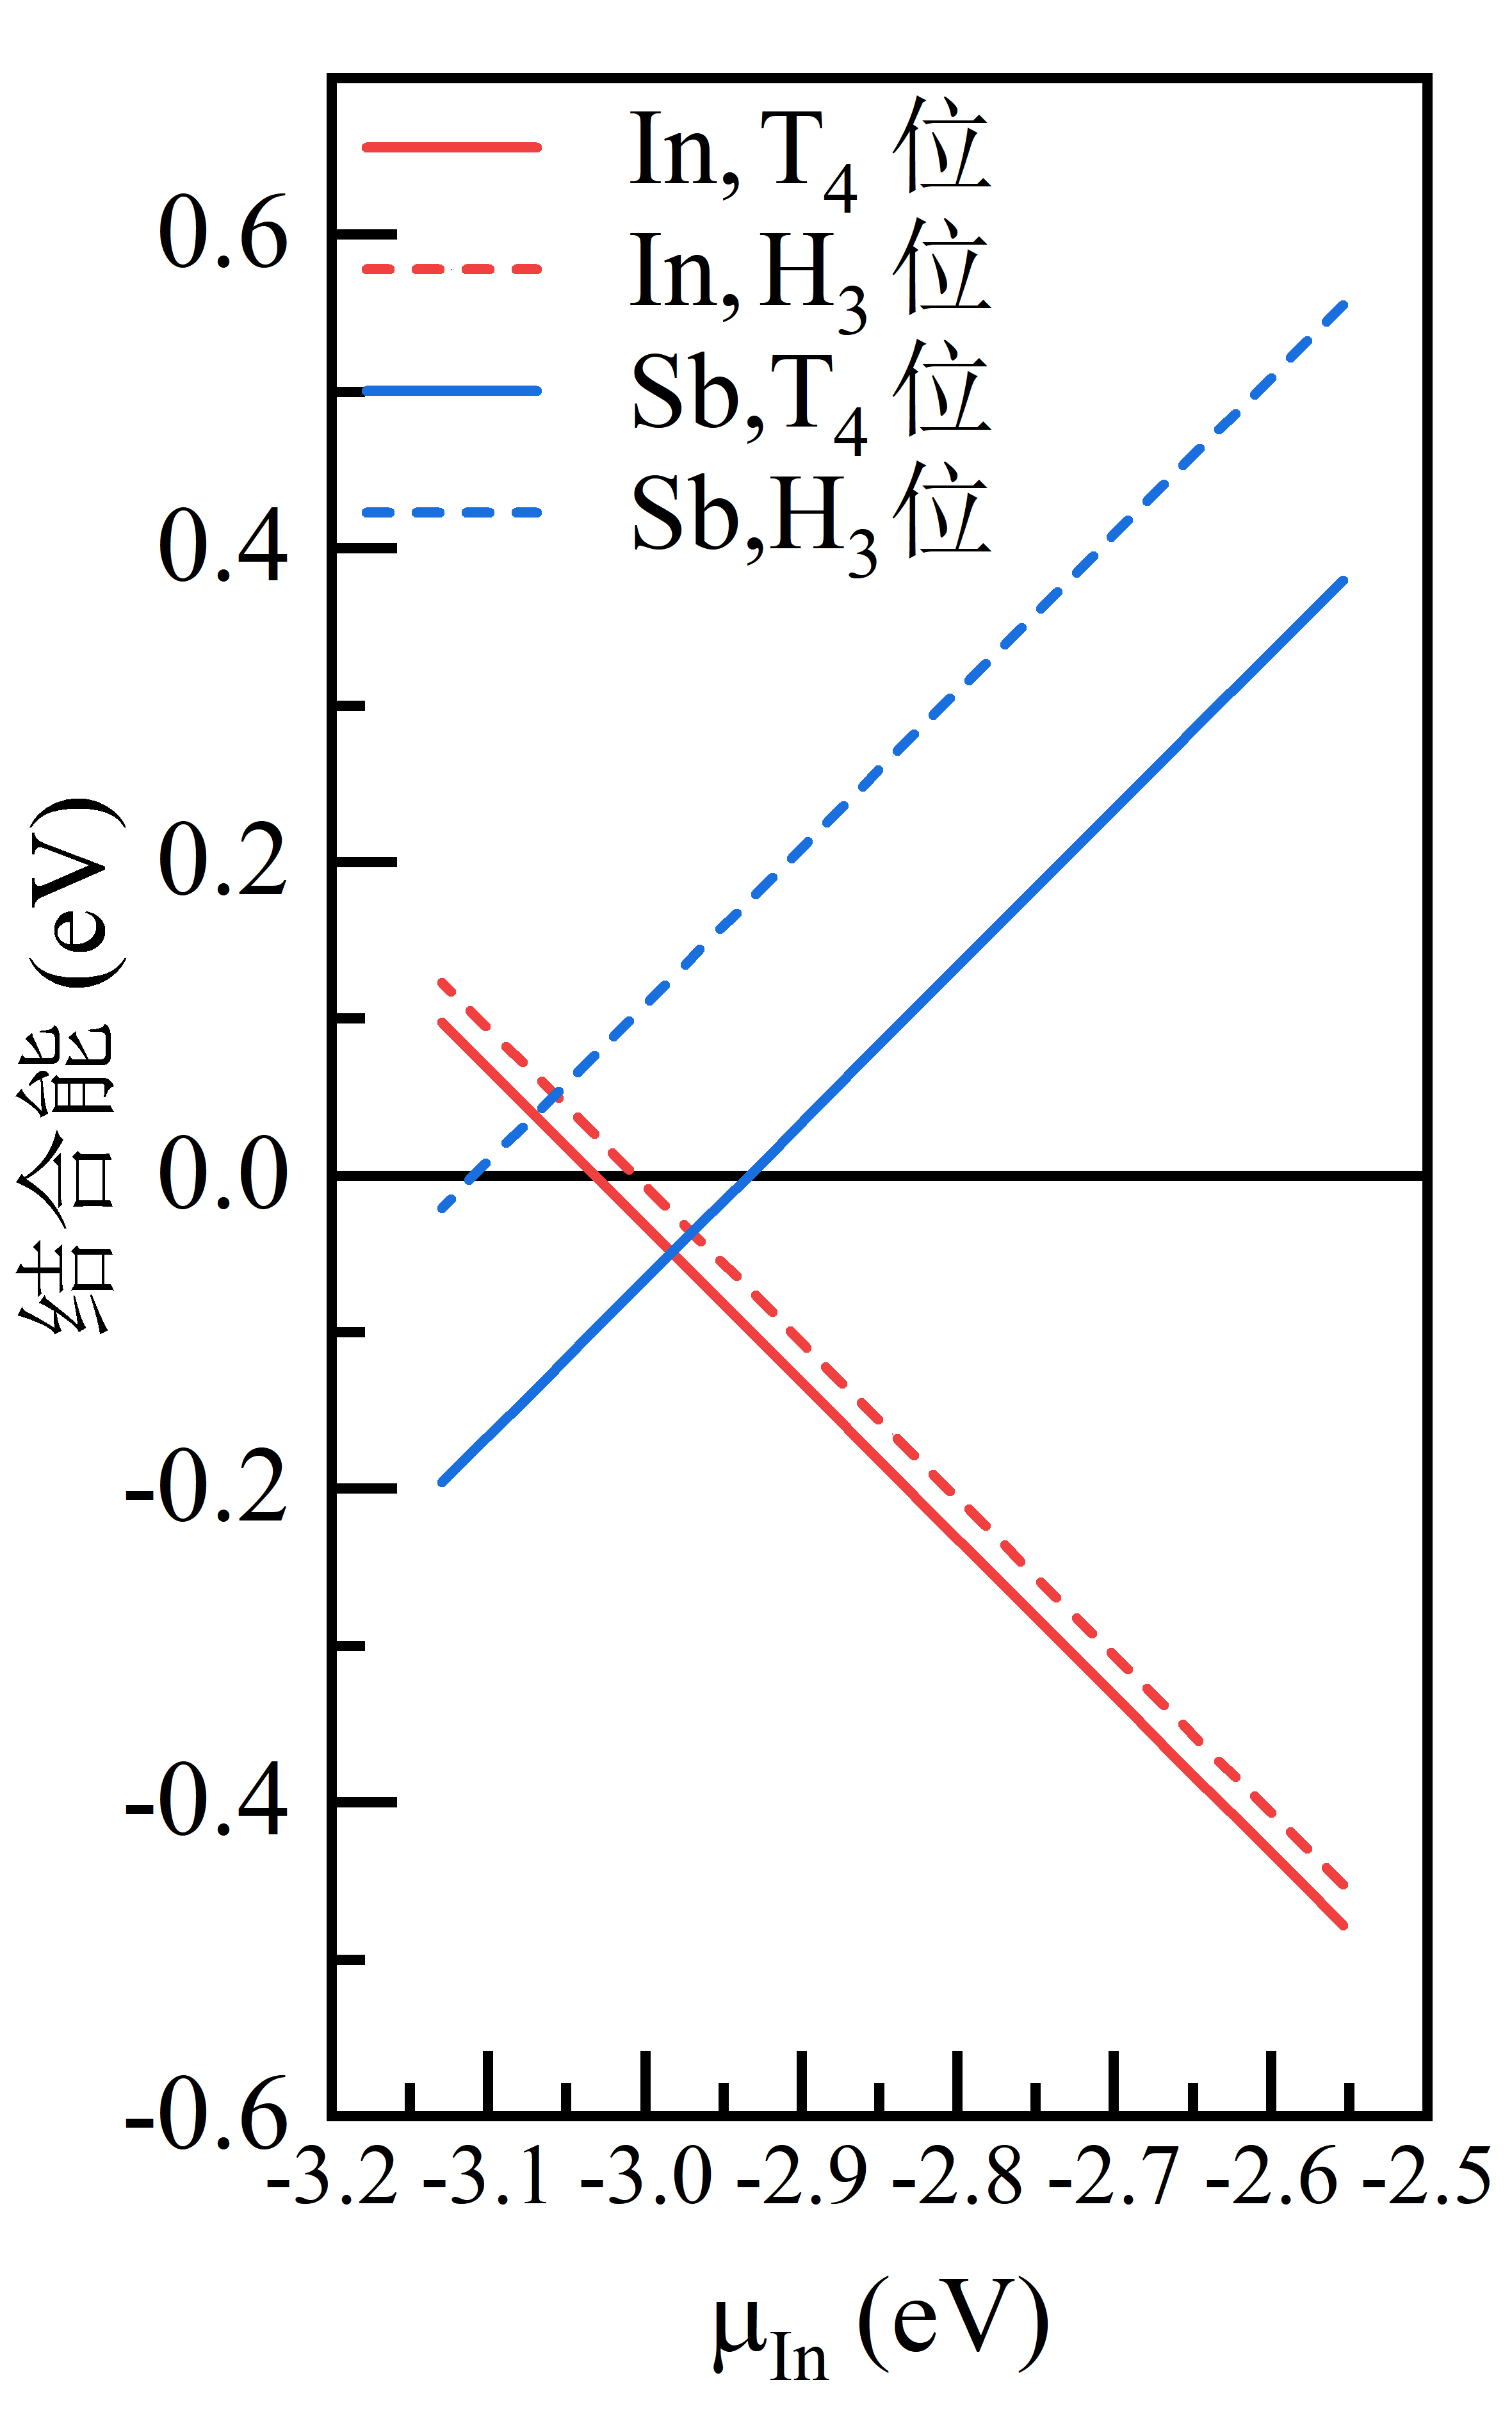
\includegraphics[]{pic/IS_DFT_adatomBind.png}
    }
    \subfloat[]{
        \label{fig:IS_structure_T4onBi}
        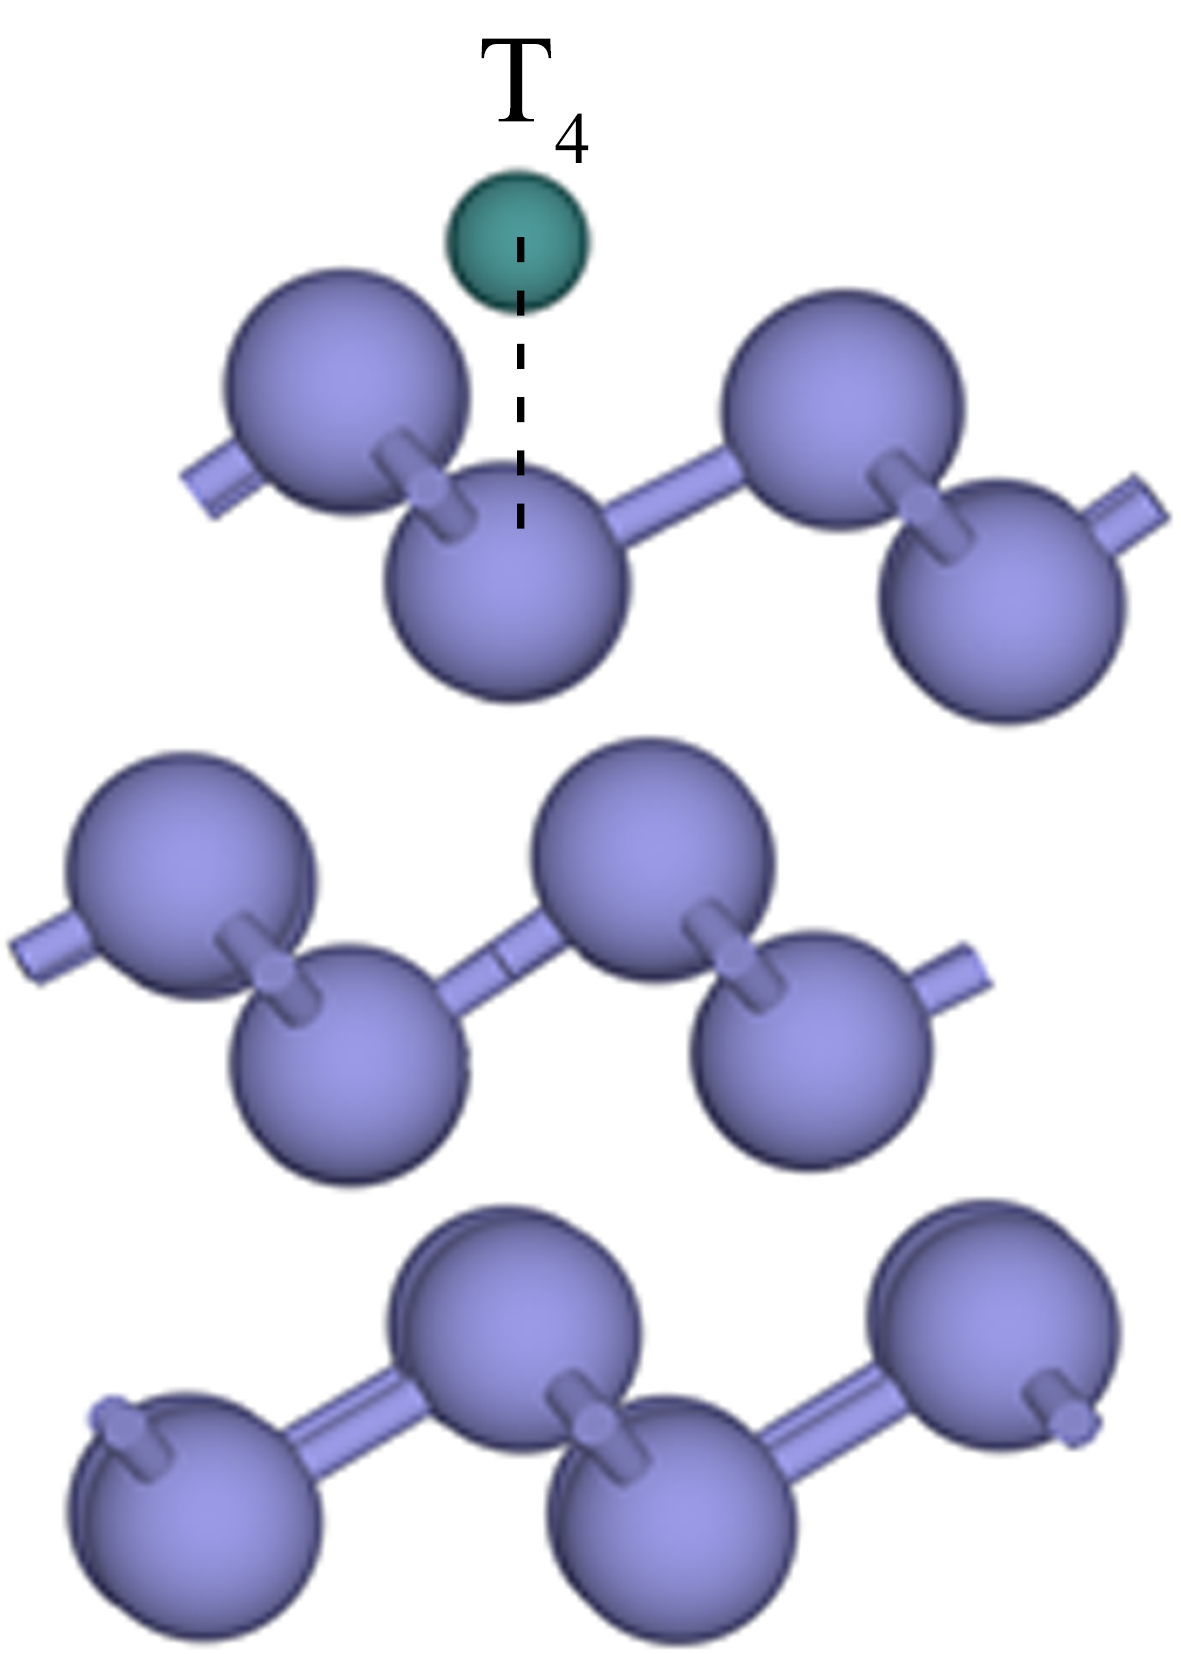
\includegraphics[width=0.3\textwidth,trim={0, -20, 0 0},clip]{pic/IS_structure_T4onBi.png}
    }
    \subfloat[]{
        \label{fig:IS_structure_H3onBi}
        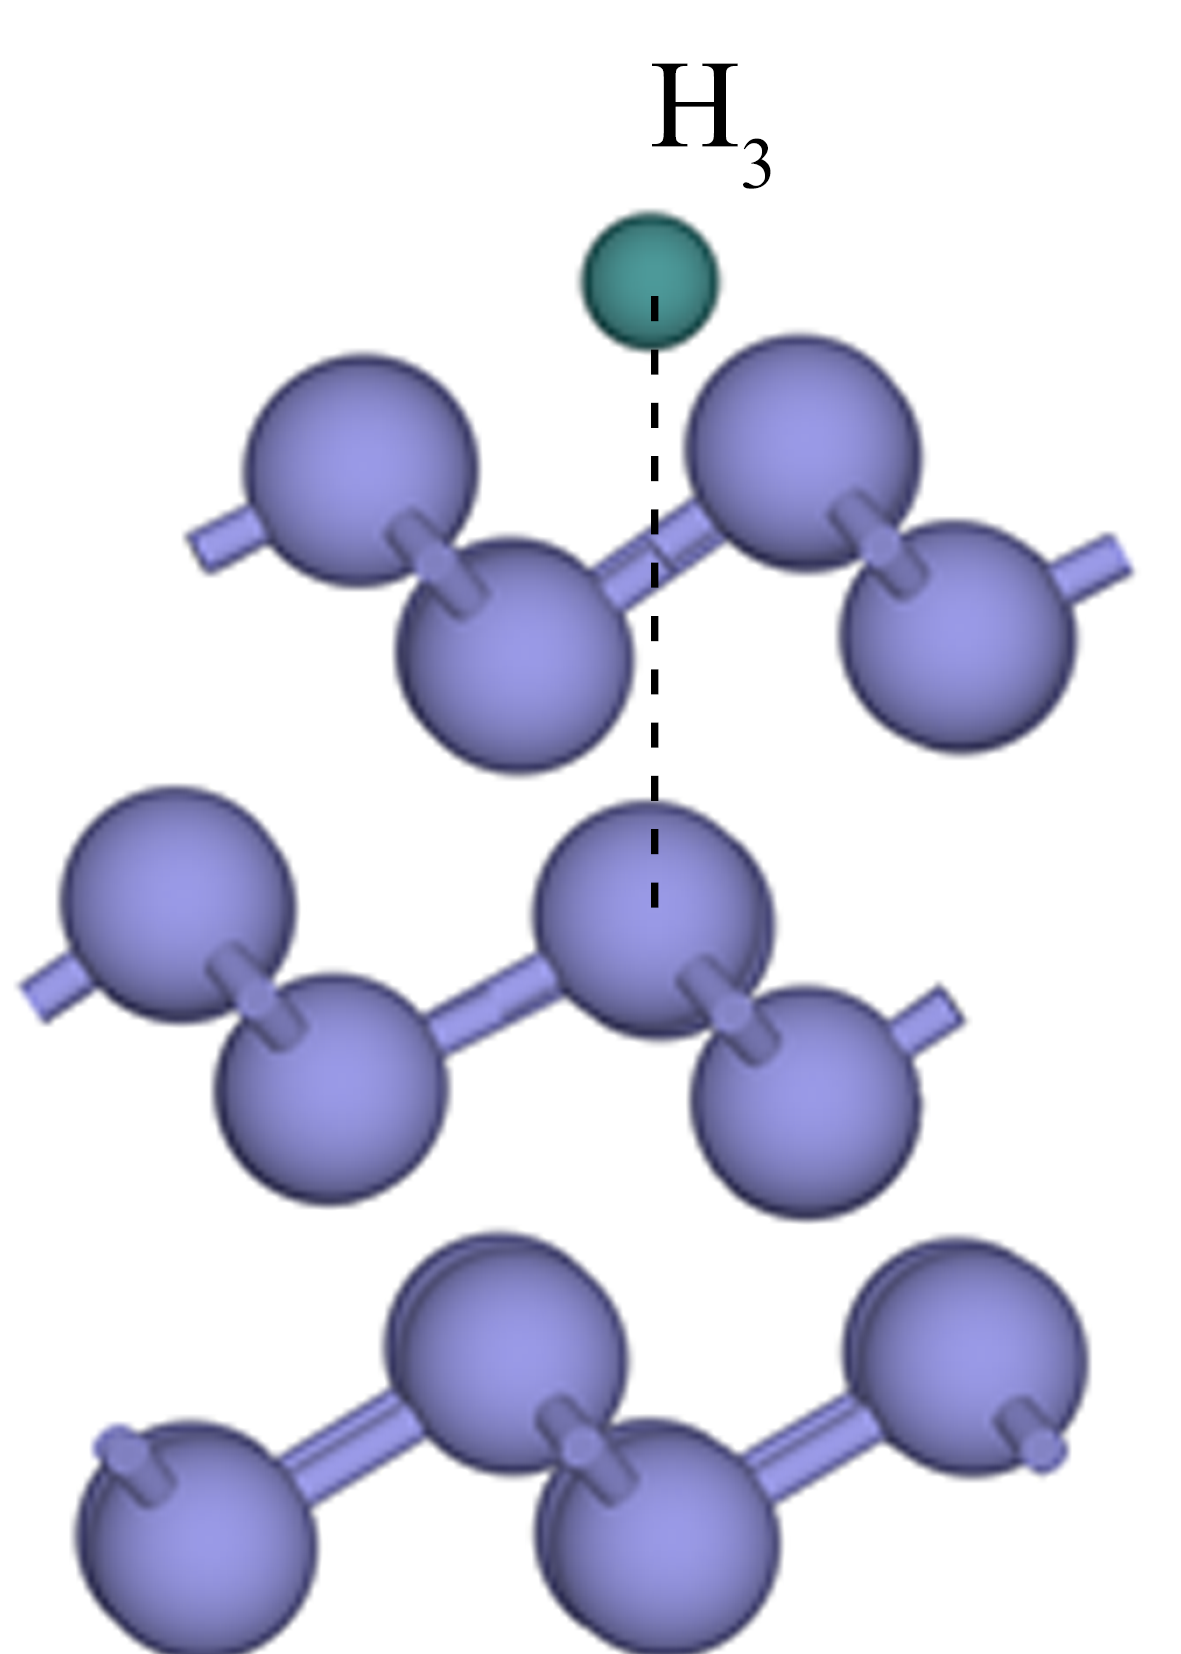
\includegraphics[width=0.3\textwidth,trim={0, -20, 0 0},clip]{pic/IS_structure_H3onBi.png}
    }
    \caption{\cemb{Bi(001)}衬底表面\cemb{In}和\cemb{Sb}吸附原子的结合能和吸附位点。(a)吸附原子结合能;(b)吸附位点T4;(c)吸附位点H3。 原子结构图中,\cemb{Bi}原子使用蓝色表示,吸附原子(\cemb{In}、\cemb{Sb})用绿色表示。}
    \label{fig:IS_Bi_adatoms}
\end{figure}

对于$\muVar{adatom}{}$为吸附原子的化学势,由于生长环境下\cemb{InSb}块体的化学平衡,我们有\chinesecolon
\begin{equation}
    \label{eq:IS_bulkEqmb}
    \muVar{In}{}+\muVar{Sb}{}=\energyVar{InSb}{tot}=\energyVar{In\left(Bulk\right)}{}+\energyVar{Sb\left(Bulk\right)}{}+\Delta H_{f}\left(\cemb{InSb}\right)
\end{equation}

其中$\energyVar{InSb}{tot}$、$\energyVar{In\left(Bulk\right)}{}$和$\energyVar{Sb\left(Bulk\right)}{}$为\cemb{InSb}块体,\cemb{In}块体和\cemb{Sb}块体的能量。因此,在生长气氛中\cemb{InSb}的化学平衡下,$\muVar{In}{}$的变化范围为$\muVar{In}{}\leqslant \energyVar{Sb\left(Bulk\right)}{}+\Delta H_{\rm f}\left(\cemb{InSb}\right) \leqslant \energyVar{In\left(Bulk\right)}{}$,代表\cemb{In}的化学势$\muVar{In}{}$由纯\cemb{Sb}的生长环境变化到纯\cemb{In}的生长环境。

对于吸附在$\TfourSite$位点的\cemb{In}原子,计算所得的在纯\cemb{In}环境下的结合能为\SI{-0.48}{\electronvolt},低于在纯\cemb{Sb}环境下同样吸附在$\TfourSite$位点的\cemb{Sb}原子的结合能(\SI{-0.19}{\electronvolt})。更抵的结合能意味着相比于\cemb{Sb}原子,在能量最低的驱动下有更多的\cemb{In}原子从块体的状态分离并以吸附原子的状态沉积到\cemb{Bi(001)}的表面。对于\cemb{In}原子来说,其在最优吸附位点$\TfourSite$的结合能只比吸附次优吸附位点$\HthreeSite$的结合能低\SI{0.026}{\electronvolt}。而对于\cemb{Sb}原子,其在次优吸附点$\HthreeSite$和最优吸附点$\TfourSite$之间的结合能之差为\SI{0.17}{\electronvolt}。由于\cemb{Sb}原子在次优吸附位点$\HthreeSite$较差的吸附能力,\cemb{Sb}原子只能在接近纯\cemb{Sb}的生长环境中在\cemb{Bi(001)}表面的$\HthreeSite$位点吸附。

进一步考虑生长环境中的化学计量比的变化对于原子吸附的影响。在图\ref{fig:IS_DFT_adatomBind}中可以看到,只有很小的$\muVar{In}{}$区间允许\cemb{In}和\cemb{Sb}同时在\cemb{Bi(001)}衬底表面吸附($\energyVar{f}{} \leqslant 0$)。在这个区间内\cemb{In}原子可以在$\TfourSite$和$\HthreeSite$位点吸附,而\cemb{Sb}原子只能在$\HthreeSite$位点吸附。对于\cemb{In}原子,由于较低的吸附能,相比于\cemb{Sb}原子其能够在较宽的$\muVar{In}{}$区间内在\cemb{Sb}衬底表面吸附。当环境中的\cemb{In}原子化学势稍微向纯\cemb{In}环境倾斜时($\muVar{In}{}\geqslant \SI{-2.9}{\electronvolt}$),仅有\cemb{In}能够在\cemb{Bi}的表面吸附,而\cemb{Sb}原子则由于大于零的结合能倾向于从\cemb{Bi}的表面脱附。

由于\cemb{In}原子和\cemb{Sb}原子在\cemb{Bi(001)}表面不同的吸附行为,在相同的化学气氛下,\cemb{In}和\cemb{Sb}很难同时在\cemb{Bi}衬底的表面独立吸附。出于更高的吸附能力,\cemb{In}在\cemb{InSb}的初期成核生长过程中处于更加主导的地位。在\cemb{In}原子能够沉积的区域,气氛中的\cemb{Sb}原子需要与已吸附的\cemb{In}原子成键、成核,才能够在\cemb{Bi}衬底的表面形成\cemb{InSb}。

我们进一步计算了\cemb{In}和\cemb{Sb}原子吸附在\cemb{Bi(001)}表面后的迁移势垒。如图\ref{fig:IS_DFT_adatomDiff}所示,对于吸附在\cemb{Bi}衬底表面的\cemb{In},其在两个等效的最优吸附$\TfourSite$位点之间迁移的势垒为\SI{0.20}{\electronvolt}。对于\cemb{Sb}原子,其在同样的最优位点$\TfourSite$之间的迁移势垒略低,为$\SI{0.19}{\electronvolt}$。而对于吸附在次优吸附位点$\HthreeSite$的\cemb{Sb}原子,只需要跨越\SI{0.018}{\electronvolt}的势垒就可迁移至最优的$\TfourSite$位点。吸附在$\HthreeSite$位点的\cemb{In}原子需要跨越约\SI{0.17}{\electronvolt}的势垒即可可迁移至能量更有优势的$\HthreeSite$位点。考虑到\cemb{In}原子在最优吸附位点$\TfourSite$和次优吸附位点$\HthreeSite$之间的能量差只有\SI{0.026}{\electronvolt},并且\cemb{In}原子和\cemb{Sb}原子在\cemb{Bi(001)}表面较低的迁移势垒,吸附的\cemb{In}原子在$\TfourSite$和$\HthreeSite$近似于均匀分布。而\cemb{Sb}原子由于在$\TfourSite$位点具有约\SI{0.17}{\electronvolt}的能量优势,因此\cemb{Sb}原子在$\TfourSite$位点吸附的比例较高。

\begin{figure}[htb]
    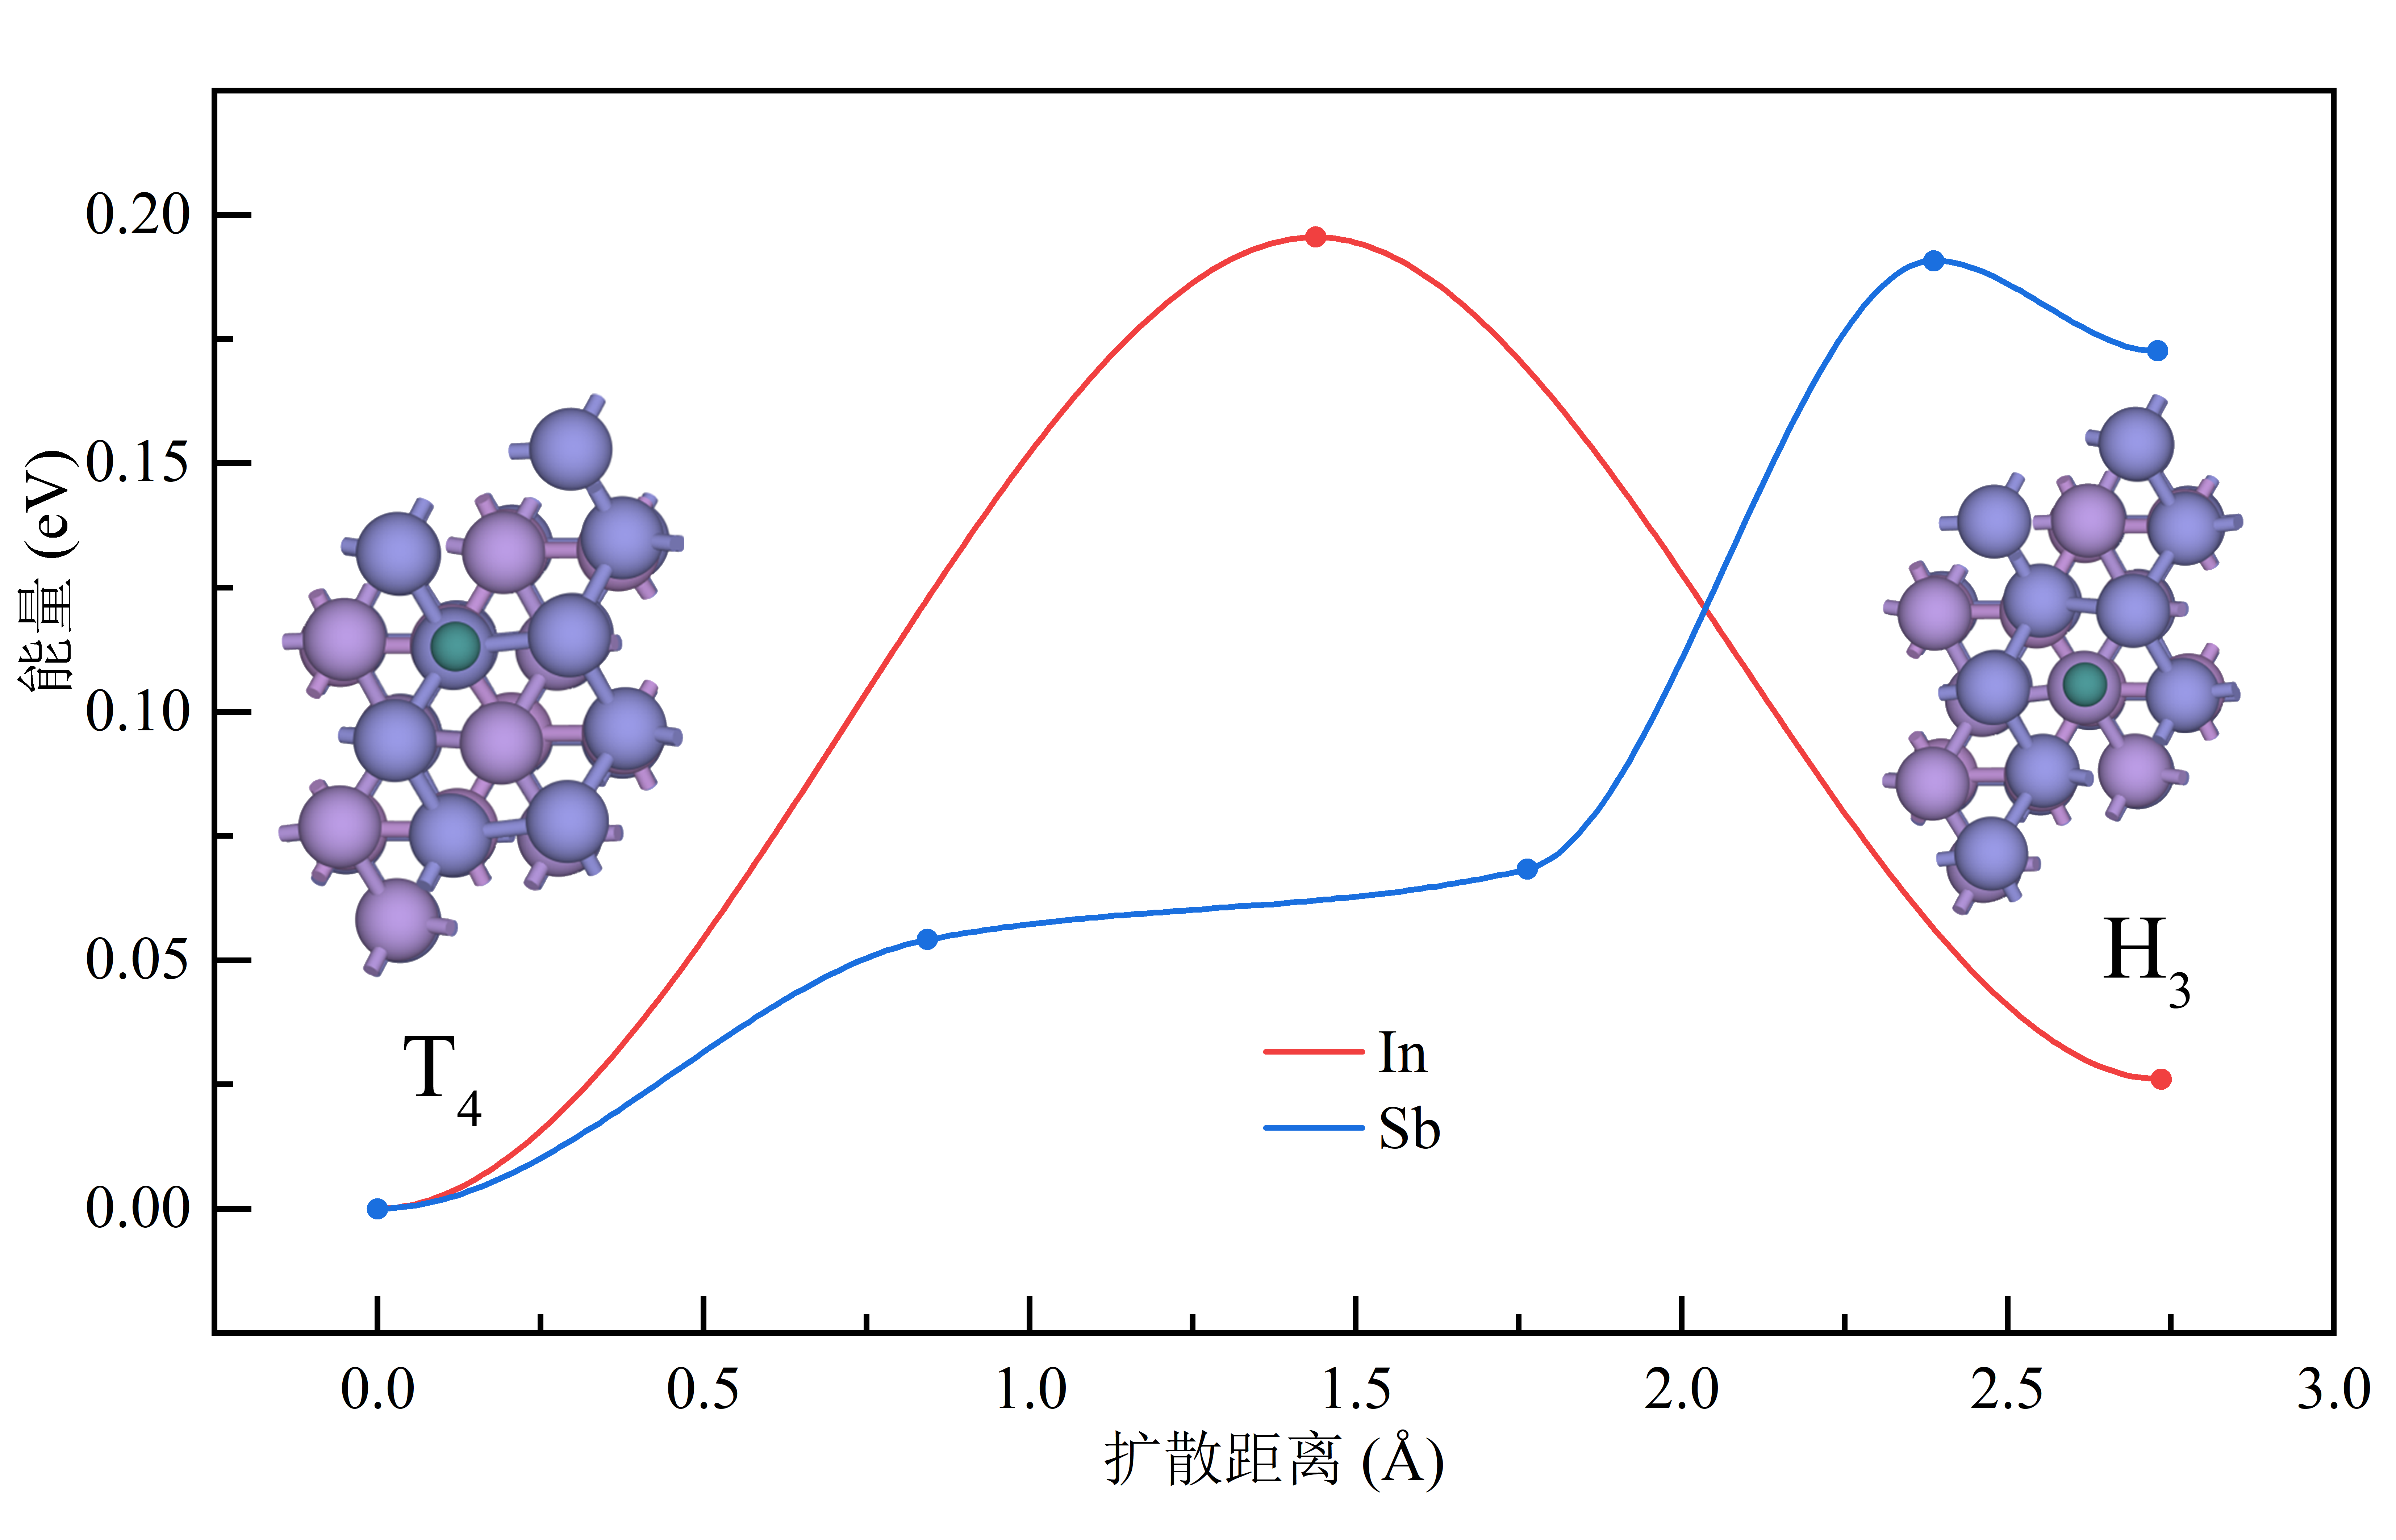
\includegraphics{pic/IS_DFT_adatomDiff.png}
    \caption{\cemb{Bi(001)}衬底表面\cemb{In}和\cemb{Sb}吸附原子的迁移势垒。原子结构图中,\cemb{Bi}原子使用蓝色表示,吸附原子(\cemb{In}、\cemb{Sb})用绿色表示。}
    \label{fig:IS_DFT_adatomDiff}
\end{figure}

为了能进一步探究\cemb{InSb(111)}在\cemb{Bi(001)}衬底上的层状生长机理以及极性的演化过程,我们计算了单层\cemb{InSb}在\cemb{Bi(001)}衬底上的形成能$\energyVar{f}{}$\chinesecolon
\begin{equation}
    \label{eq:IS_formationEnenrgy}
    \energyVar{f}{}=\frac{1}{\alpha}\left(\energyVar{\cemb{InSb}+sub}{}-\energyVar{sub}{}-N_{\rm In}\muVar{In}{}-N_{\rm Sb}\muVar{Sb}{}\right)
\end{equation}

其中,$\alpha$为模拟体系的表面积;$\energyVar{\cemb{InSb}+sub}{}$和$\energyVar{sub}{}$分别为在衬底表面生长了一层\cemb{InSb}的能量以及单独衬底的能量;$N_{\rm In}$和$N_{\rm Sb}$分别为\cemb{InSb}单层中\cemb{In}和\cemb{Sb}原子的数量。

我们首先考虑理想的\cemb{InSb}单层在\cemb{Bi(001)}衬底上的生长情况。在我们的计算中,无论是\cemb{In}极性的\cemb{InSb(111)}单层还是\cemb{Sb}极性,他们都倾向于在\cemb{Bi(001)}衬底表面形成面心立方的堆叠形式(fcc, ABC堆叠)。同时,这也与我们在单\cemb{In/Sb}原子的吸附计算结果一致,即\cemb{In}和\cemb{Sb}作为吸附原子更倾向于吸附在\cemb{Bi(001)}表面的$\TfourSite$位和$\HthreeSite$位。具体而言,\cemb{In}极性的\cemb{InSb(111)}单层在\cemb{Bi(001)}衬底的表面形成能为\SI{-13.74}{\mievpas},高于\cemb{Sb}极性\cemb{InSb(111)}单层的\SI{-9.40}{\mievpas}。因此,对于理想的\cemb{InSb}单层,在\cemb{Bi(001)}衬底上应生长为\cemb{In}极性。在表格\ref{tab:IS_idealInSb_formationEnergy}中,我们总结了不同极性的\cemb{InSb}单层在\cemb{Bi(001)}衬底上的形成能及原子分布。

\begin{table}[h]
    \centering
    \caption{不同极性的\cemb{InSb}单层在\cemb{Bi(001)}衬底上的形成能及原子分布}
    \begin{tabular}{cccc}
        \toprule
        极性          & 形成能(\si{\mievpas}) & \cemb{In}原子位置 & \cemb{Sb}原子位置 \\
        \midrule
        \cemb{In}极性 & -13.74                & $\TfourSite$      & $\HthreeSite$     \\
        \cemb{Sb}极性 & -9.40                 & $\HthreeSite$     & $\TfourSite$      \\
        \bottomrule
    \end{tabular}
    \label{tab:IS_idealInSb_formationEnergy}
\end{table}

\subsection{单层锑化铟的极性演化}

\begin{figure}[htb]
    \subfloat[]{
        \label{fig:IS_structure_1Linsb_04}
        \begin{tabular}{c}
            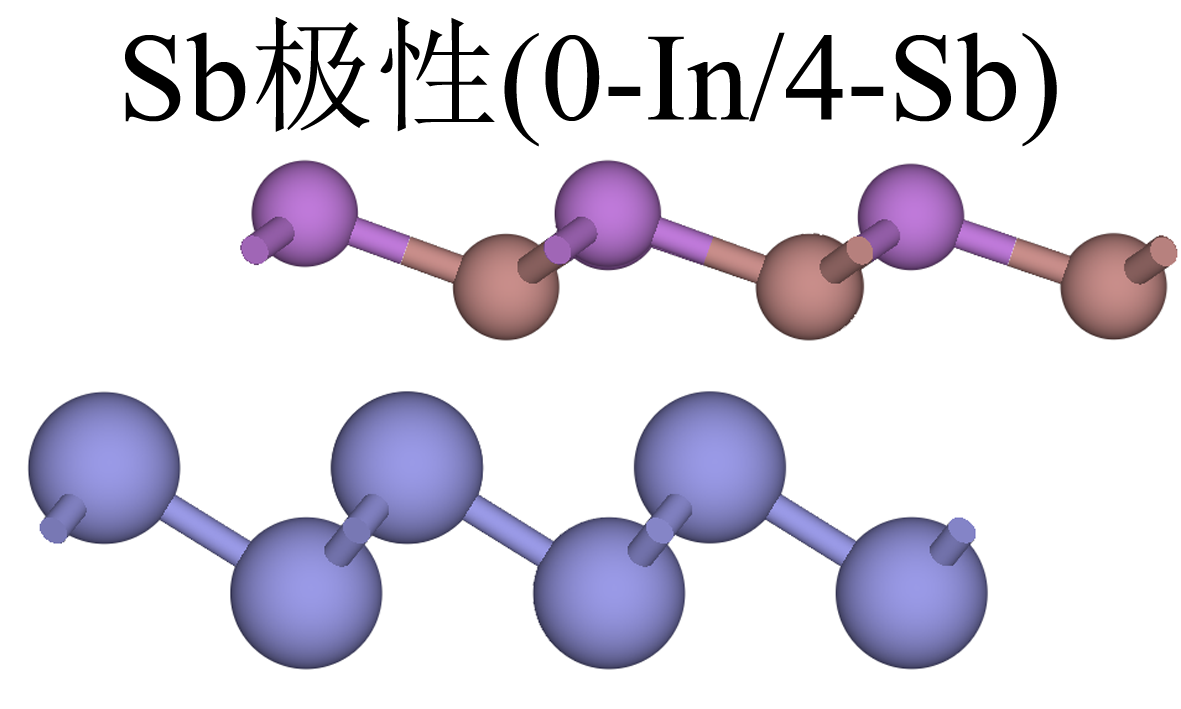
\includegraphics[width=0.28\textwidth]{pic/IS_structure_1Linsb_04side.png} \\
            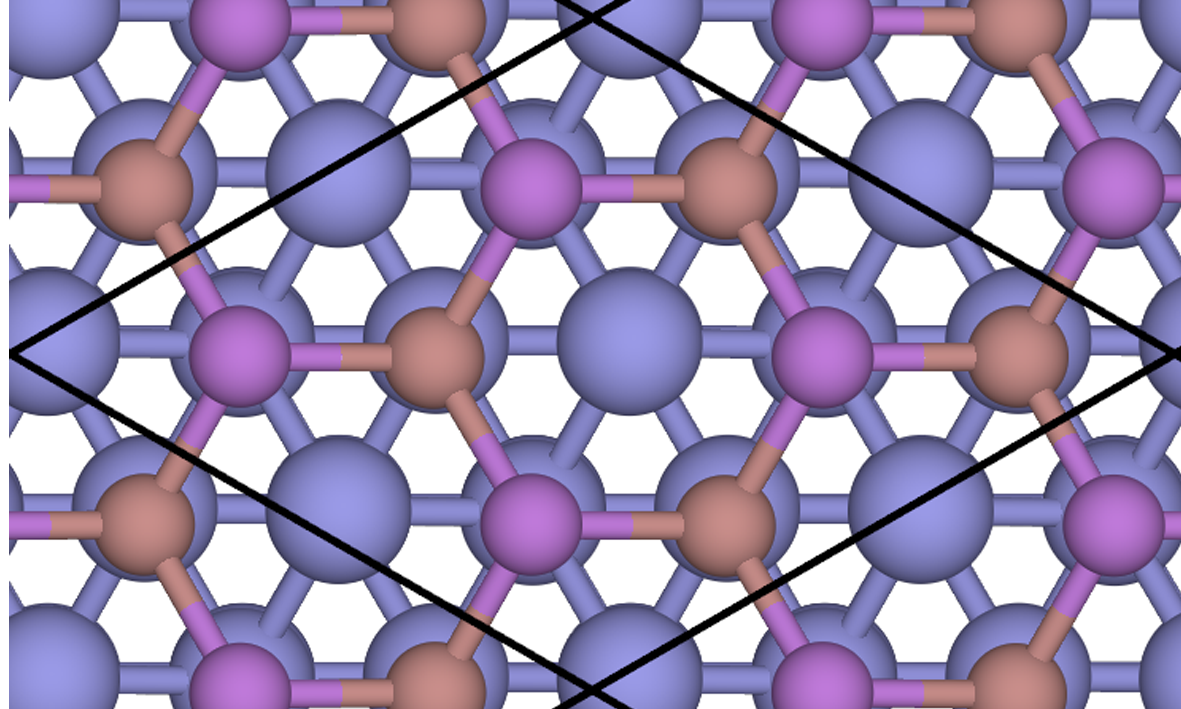
\includegraphics[width=0.28\textwidth]{pic/IS_structure_1Linsb_04top.png}
        \end{tabular}
    }
    \subfloat[]{
        \label{fig:IS_structure_1Linsb_13}
        \begin{tabular}{c}
            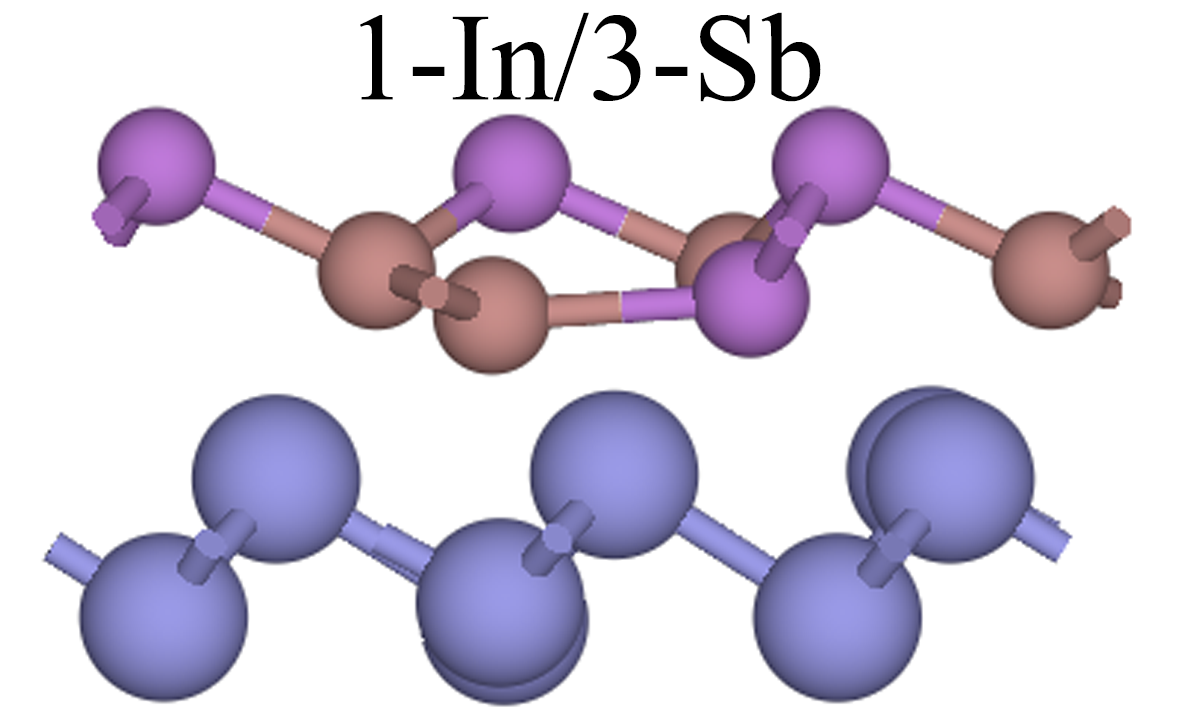
\includegraphics[width=0.28\textwidth]{pic/IS_structure_1Linsb_13side.png} \\
            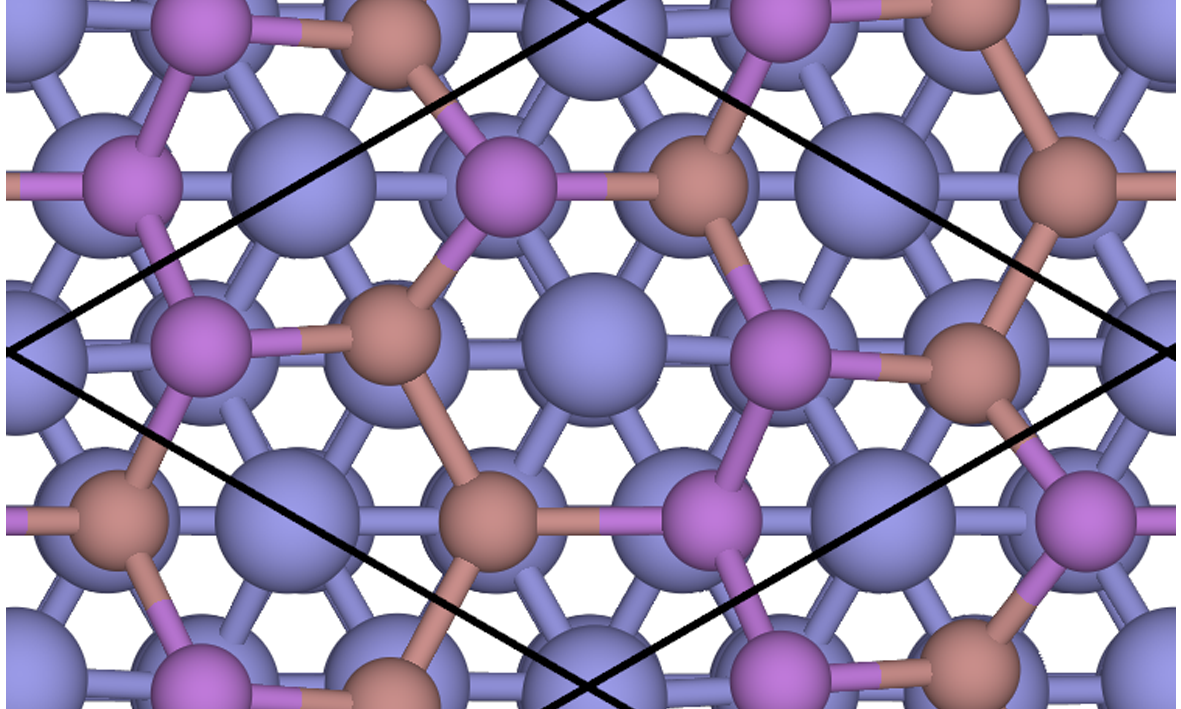
\includegraphics[width=0.28\textwidth]{pic/IS_structure_1Linsb_13top.png}
        \end{tabular}
    }
    \subfloat[]{
        \label{fig:IS_structure_1Linsb_22rec}
        \begin{tabular}{c}
            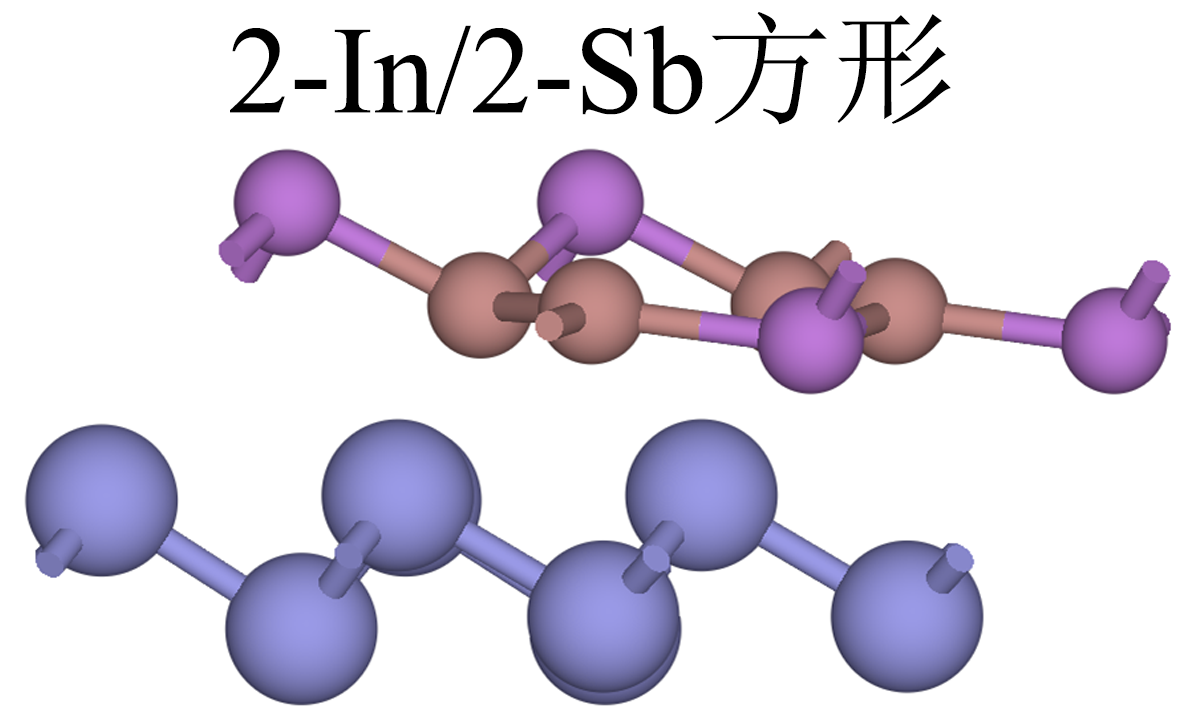
\includegraphics[width=0.28\textwidth]{pic/IS_structure_1Linsb_22recside.png} \\
            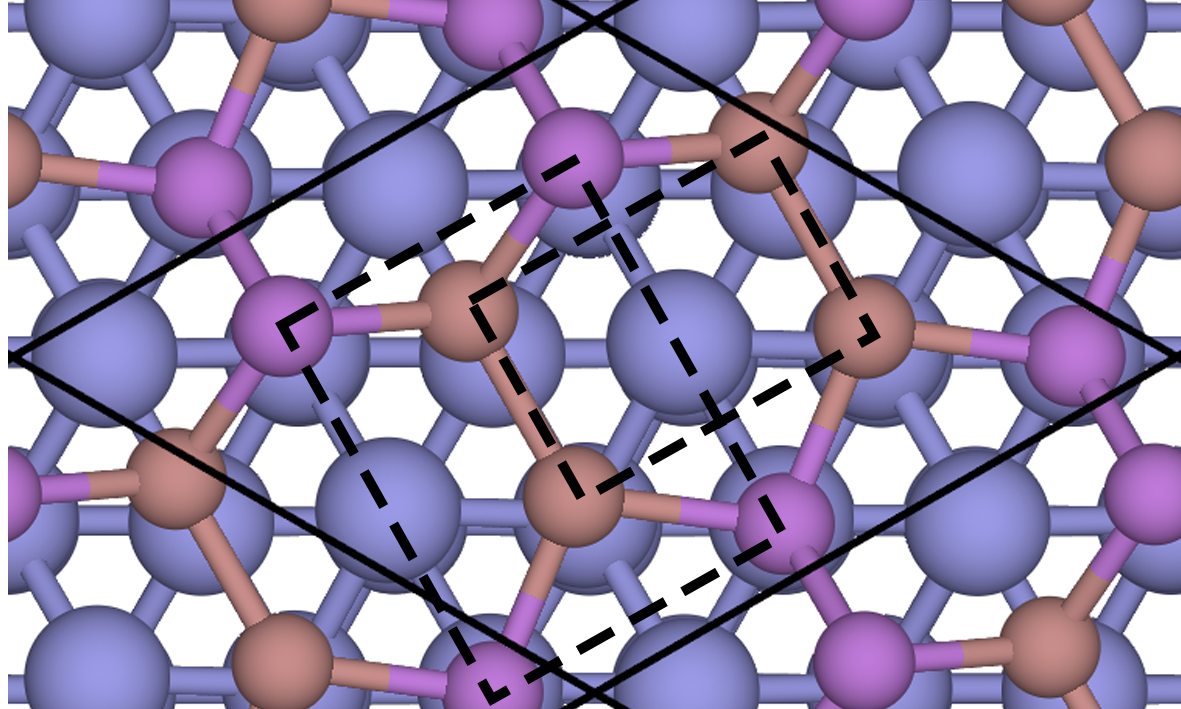
\includegraphics[width=0.28\textwidth]{pic/IS_structure_1Linsb_22rectop.png}
        \end{tabular}
    }\\[-1ex]
    \subfloat[]{
        \label{fig:IS_structure_1Linsb_22str}
        \begin{tabular}{c}
            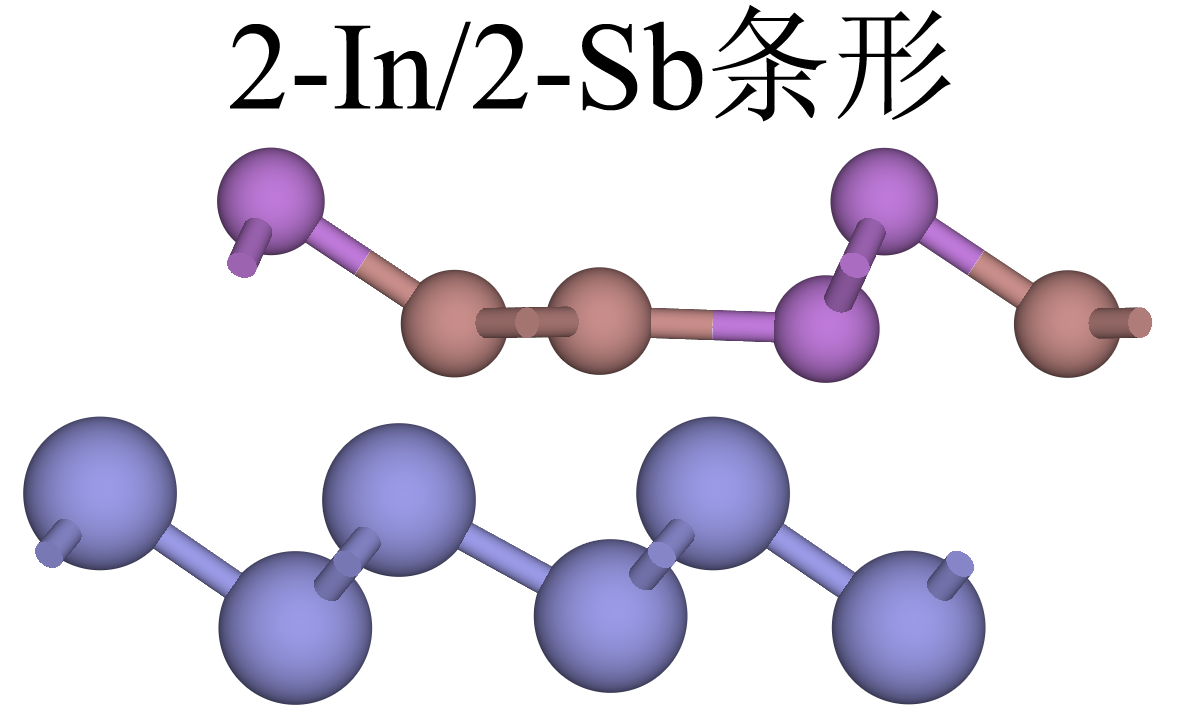
\includegraphics[width=0.28\textwidth]{pic/IS_structure_1Linsb_22strside.png} \\
            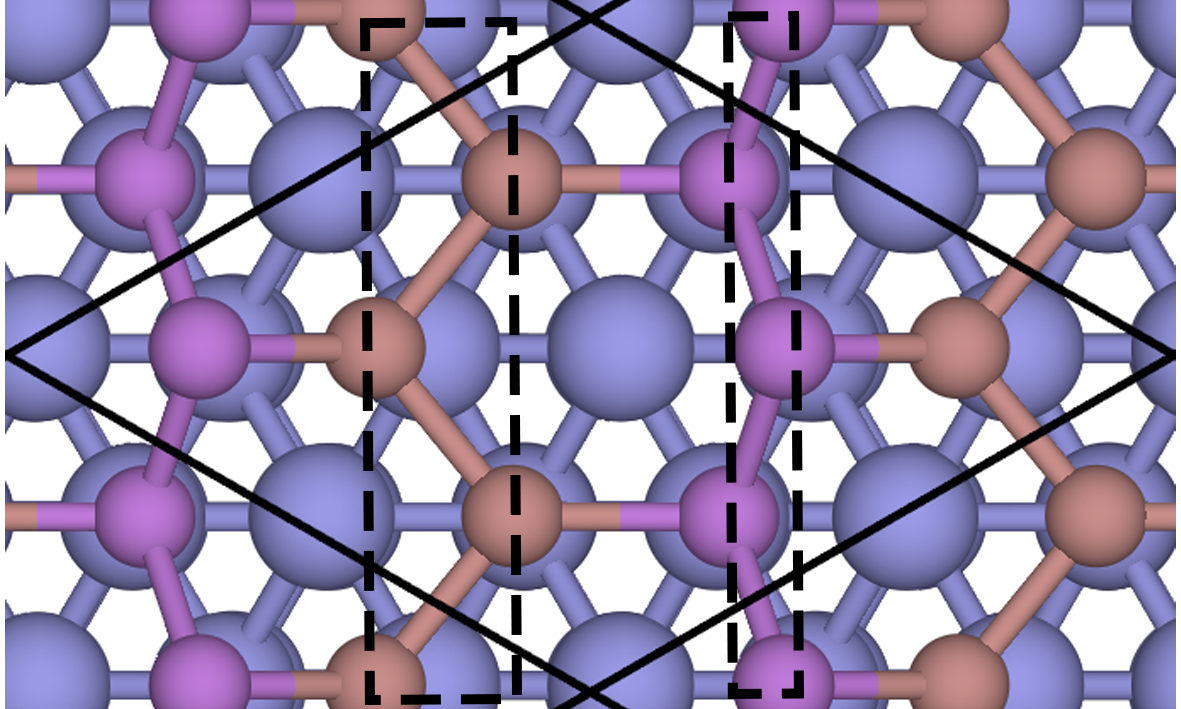
\includegraphics[width=0.28\textwidth]{pic/IS_structure_1Linsb_22strtop.png}
        \end{tabular}
    }
    \subfloat[]{
        \label{fig:IS_structure_1Linsb_31}
        \begin{tabular}{c}
            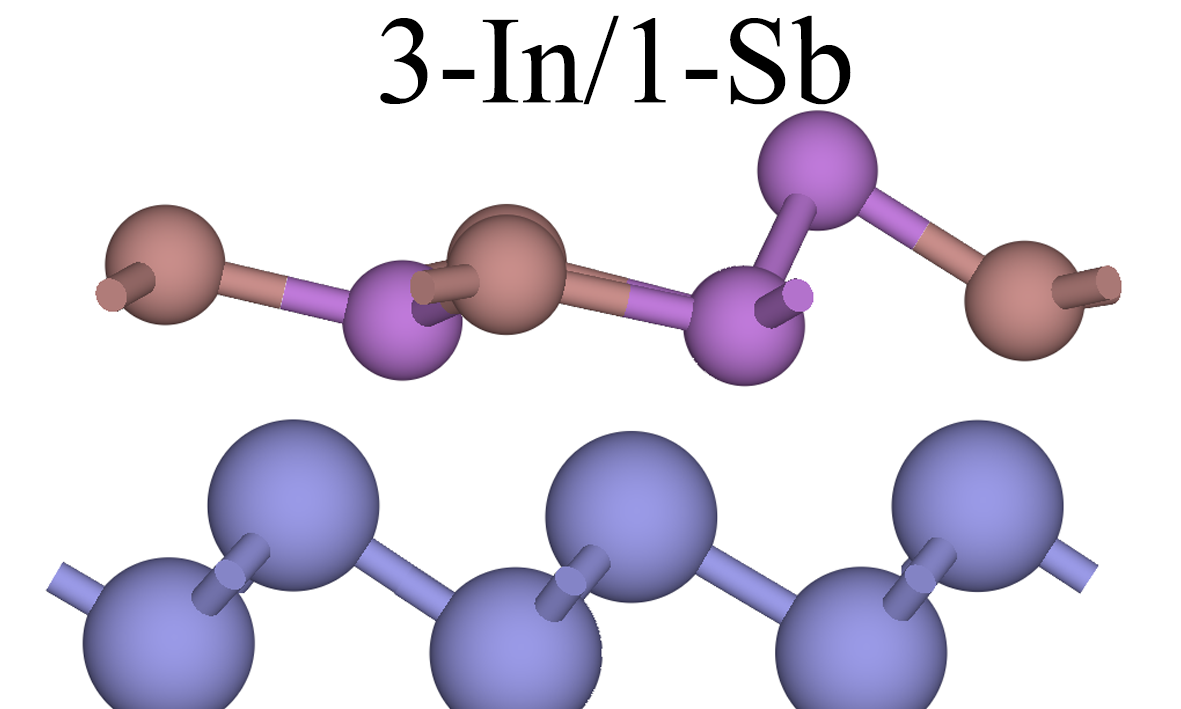
\includegraphics[width=0.28\textwidth]{pic/IS_structure_1Linsb_31side.png} \\
            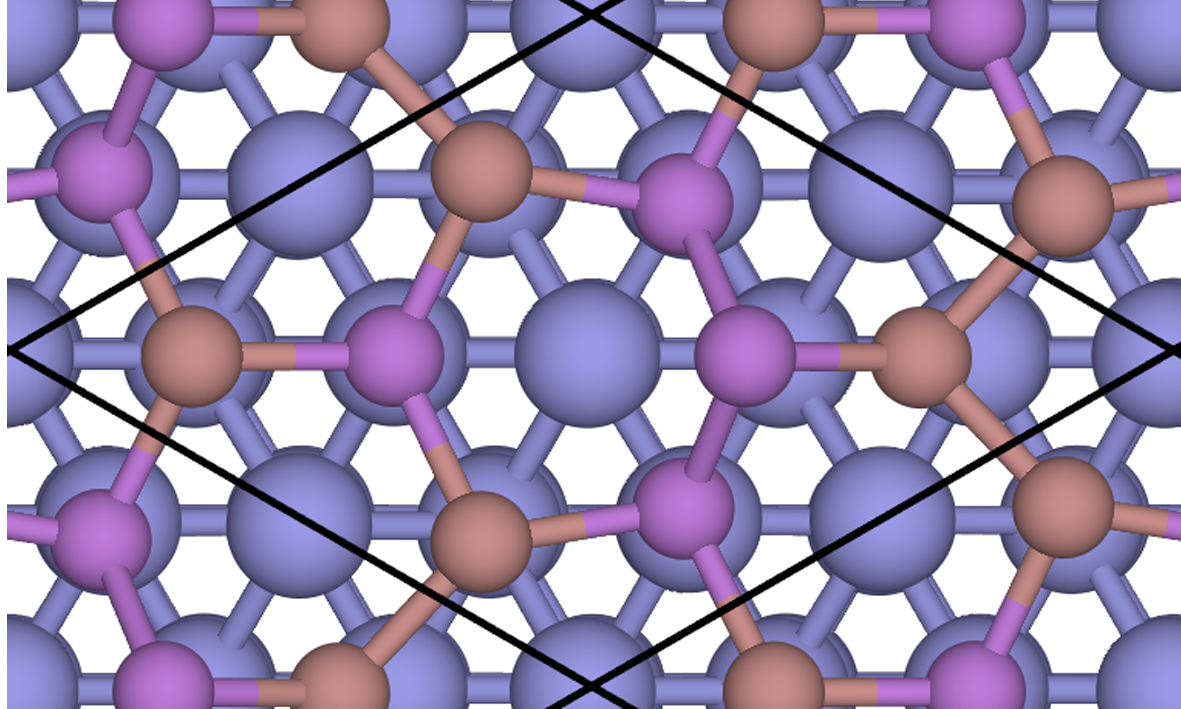
\includegraphics[width=0.28\textwidth]{pic/IS_structure_1Linsb_31top.png}
        \end{tabular}
    }
    \subfloat[]{
        \label{fig:IS_structure_1Linsb_40}
        \begin{tabular}{c}
            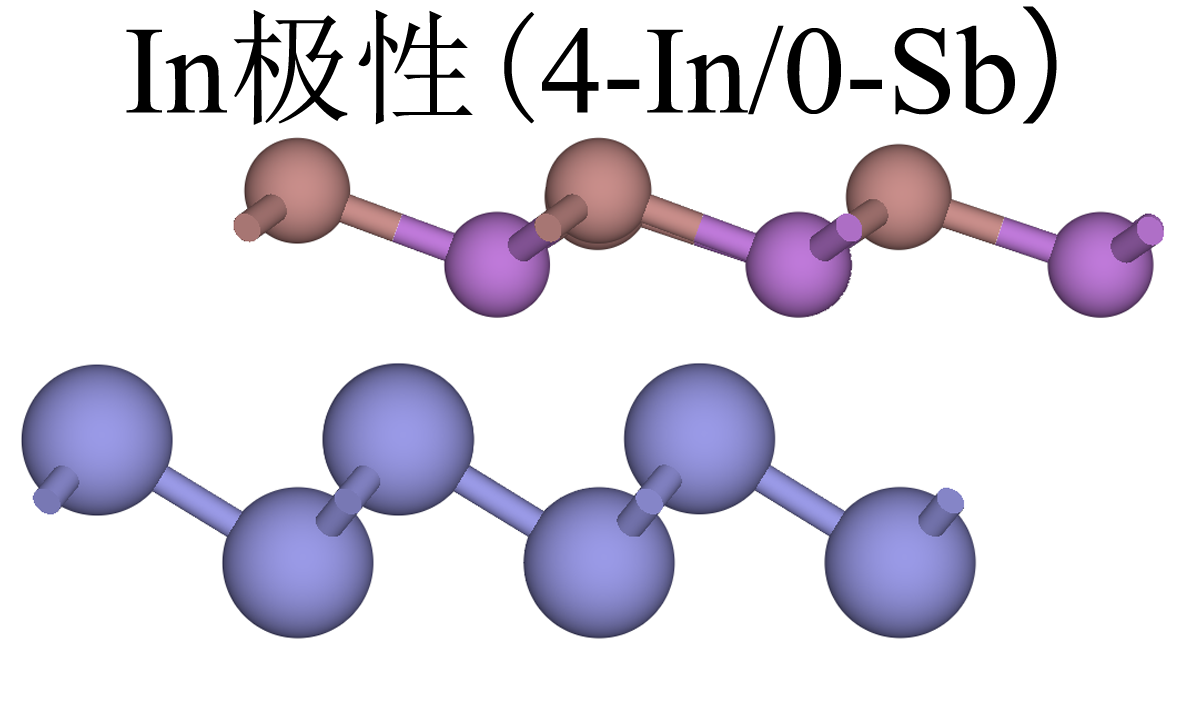
\includegraphics[width=0.28\textwidth]{pic/IS_structure_1Linsb_40side.png} \\
            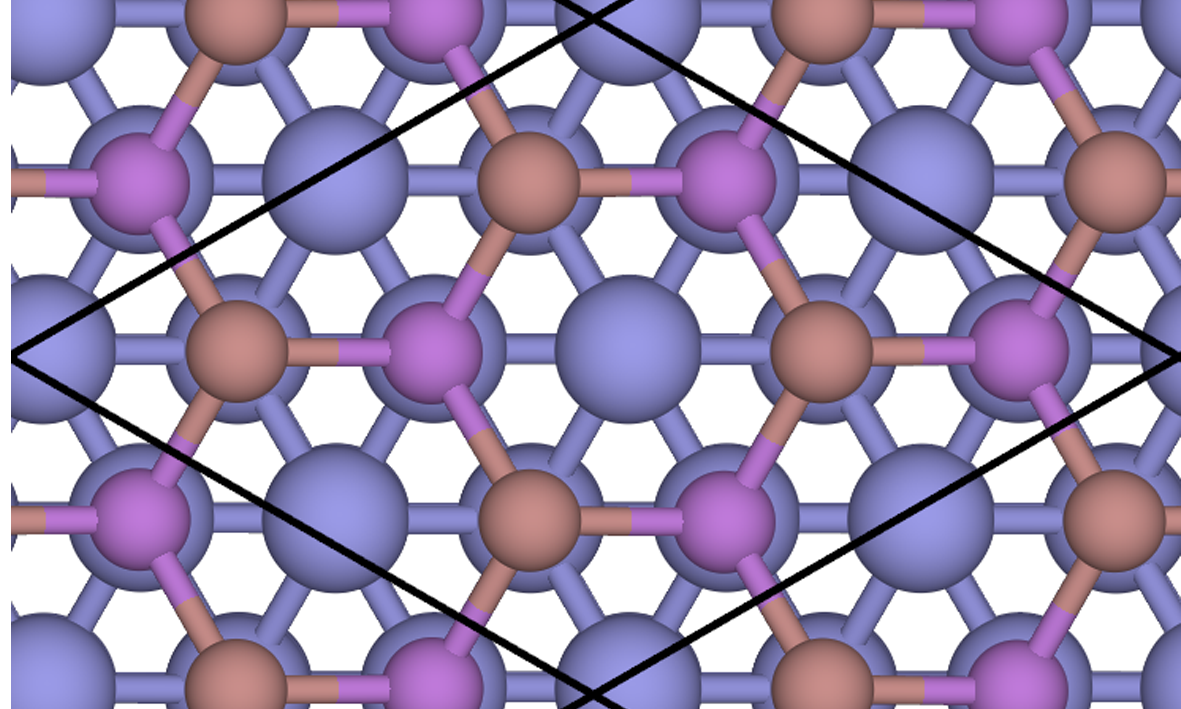
\includegraphics[width=0.28\textwidth]{pic/IS_structure_1Linsb_40top.png}
        \end{tabular}
    }
    \caption{\cemb{Bi(001)}衬底上不同极性单层\cemb{InSb}的原子结构。原子结构图中,\cemb{Bi}原子使用蓝色表示,\cemb{In}原子使用褐色表示,\cemb{Sb}原子使用紫色表示。}
    \label{fig:IS_structure_1Linsb_allPolarity}
\end{figure}

接着,我们将单层\cemb{InSb(111)}极性的考察范围扩大到非理想的情况。考虑到吸附的\cemb{In}原子和\cemb{Sb}原子均倾向于沉积在$\TfourSite$位点和$\HthreeSite$位点,使用包含四个\cemb{In}原子和四个\cemb{Sb}原子的$2 \times 2$切片模型,我们可以列举出六种可能的单层\cemb{InSb}极性。在图\ref{fig:IS_structure_1Linsb_allPolarity}中,我们列出了本章中所考虑的所有单层\cemb{InSb}的极性情况。这里,我们使用\cemb{InSb}单层中处于$\TfourSite$的原子的数量来表示不同极性的\cemb{InSb(111)}单层,例如在$2 \times 2$切片模型中理想的\cemb{In}极性\cemb{InSb}中,四个$\TfourSite$都被\cemb{In}原子占据,因此可以表示为$\InSbMLpolar{4}{0}$。相对应的,\cemb{Sb}极性的\cemb{InSb}可以表示为$\InSbMLpolar{0}{4}$。对于$\InSbMLpolar{2}{2}$极性的\cemb{InSb}单层,有两个不等价的构型。其中一个构型内部\cemb{In}原子和\cemb{Sb}分别构成两个相互嵌套的方形的四个顶角,我们用$\InSbMLpolar{2}{2}$方形表示。另一个构型中\cemb{In}原子和\cemb{Sb}原子呈条状分布,我们用$\InSbMLpolar{2}{2}$条形表示。


如图\ref{fig:IS_DFT_1LInSb_all}所示,我们计算了所有极性的$2 \times 2 \cemb{InSb}$在\cemb{Bi(001)}衬底表面的形成能。在$2 \times 2$模型中,\cemb{In}极性($\InSbMLpolar{4}{0}$)的形成能为\SI{-18.52}{\mievpas},低于$2 \times 2$模型中\cemb{Sb}极性($\InSbMLpolar{0}{4}$)的形成能(\SI{-14.64}{\mievpas})。$2 \times 2 \cemb{InSb}$理想极性(\cemb{Sb}极性和\cemb{In}极性)的计算结果与上一节中$1 \times 1$模型一致。$2 \times 2$模型中更低的形成能可能是由于表面原子在$2 \times 2$模型中有更多的空间可以进行更完全的几何优化。


\begin{figure}[htb]
    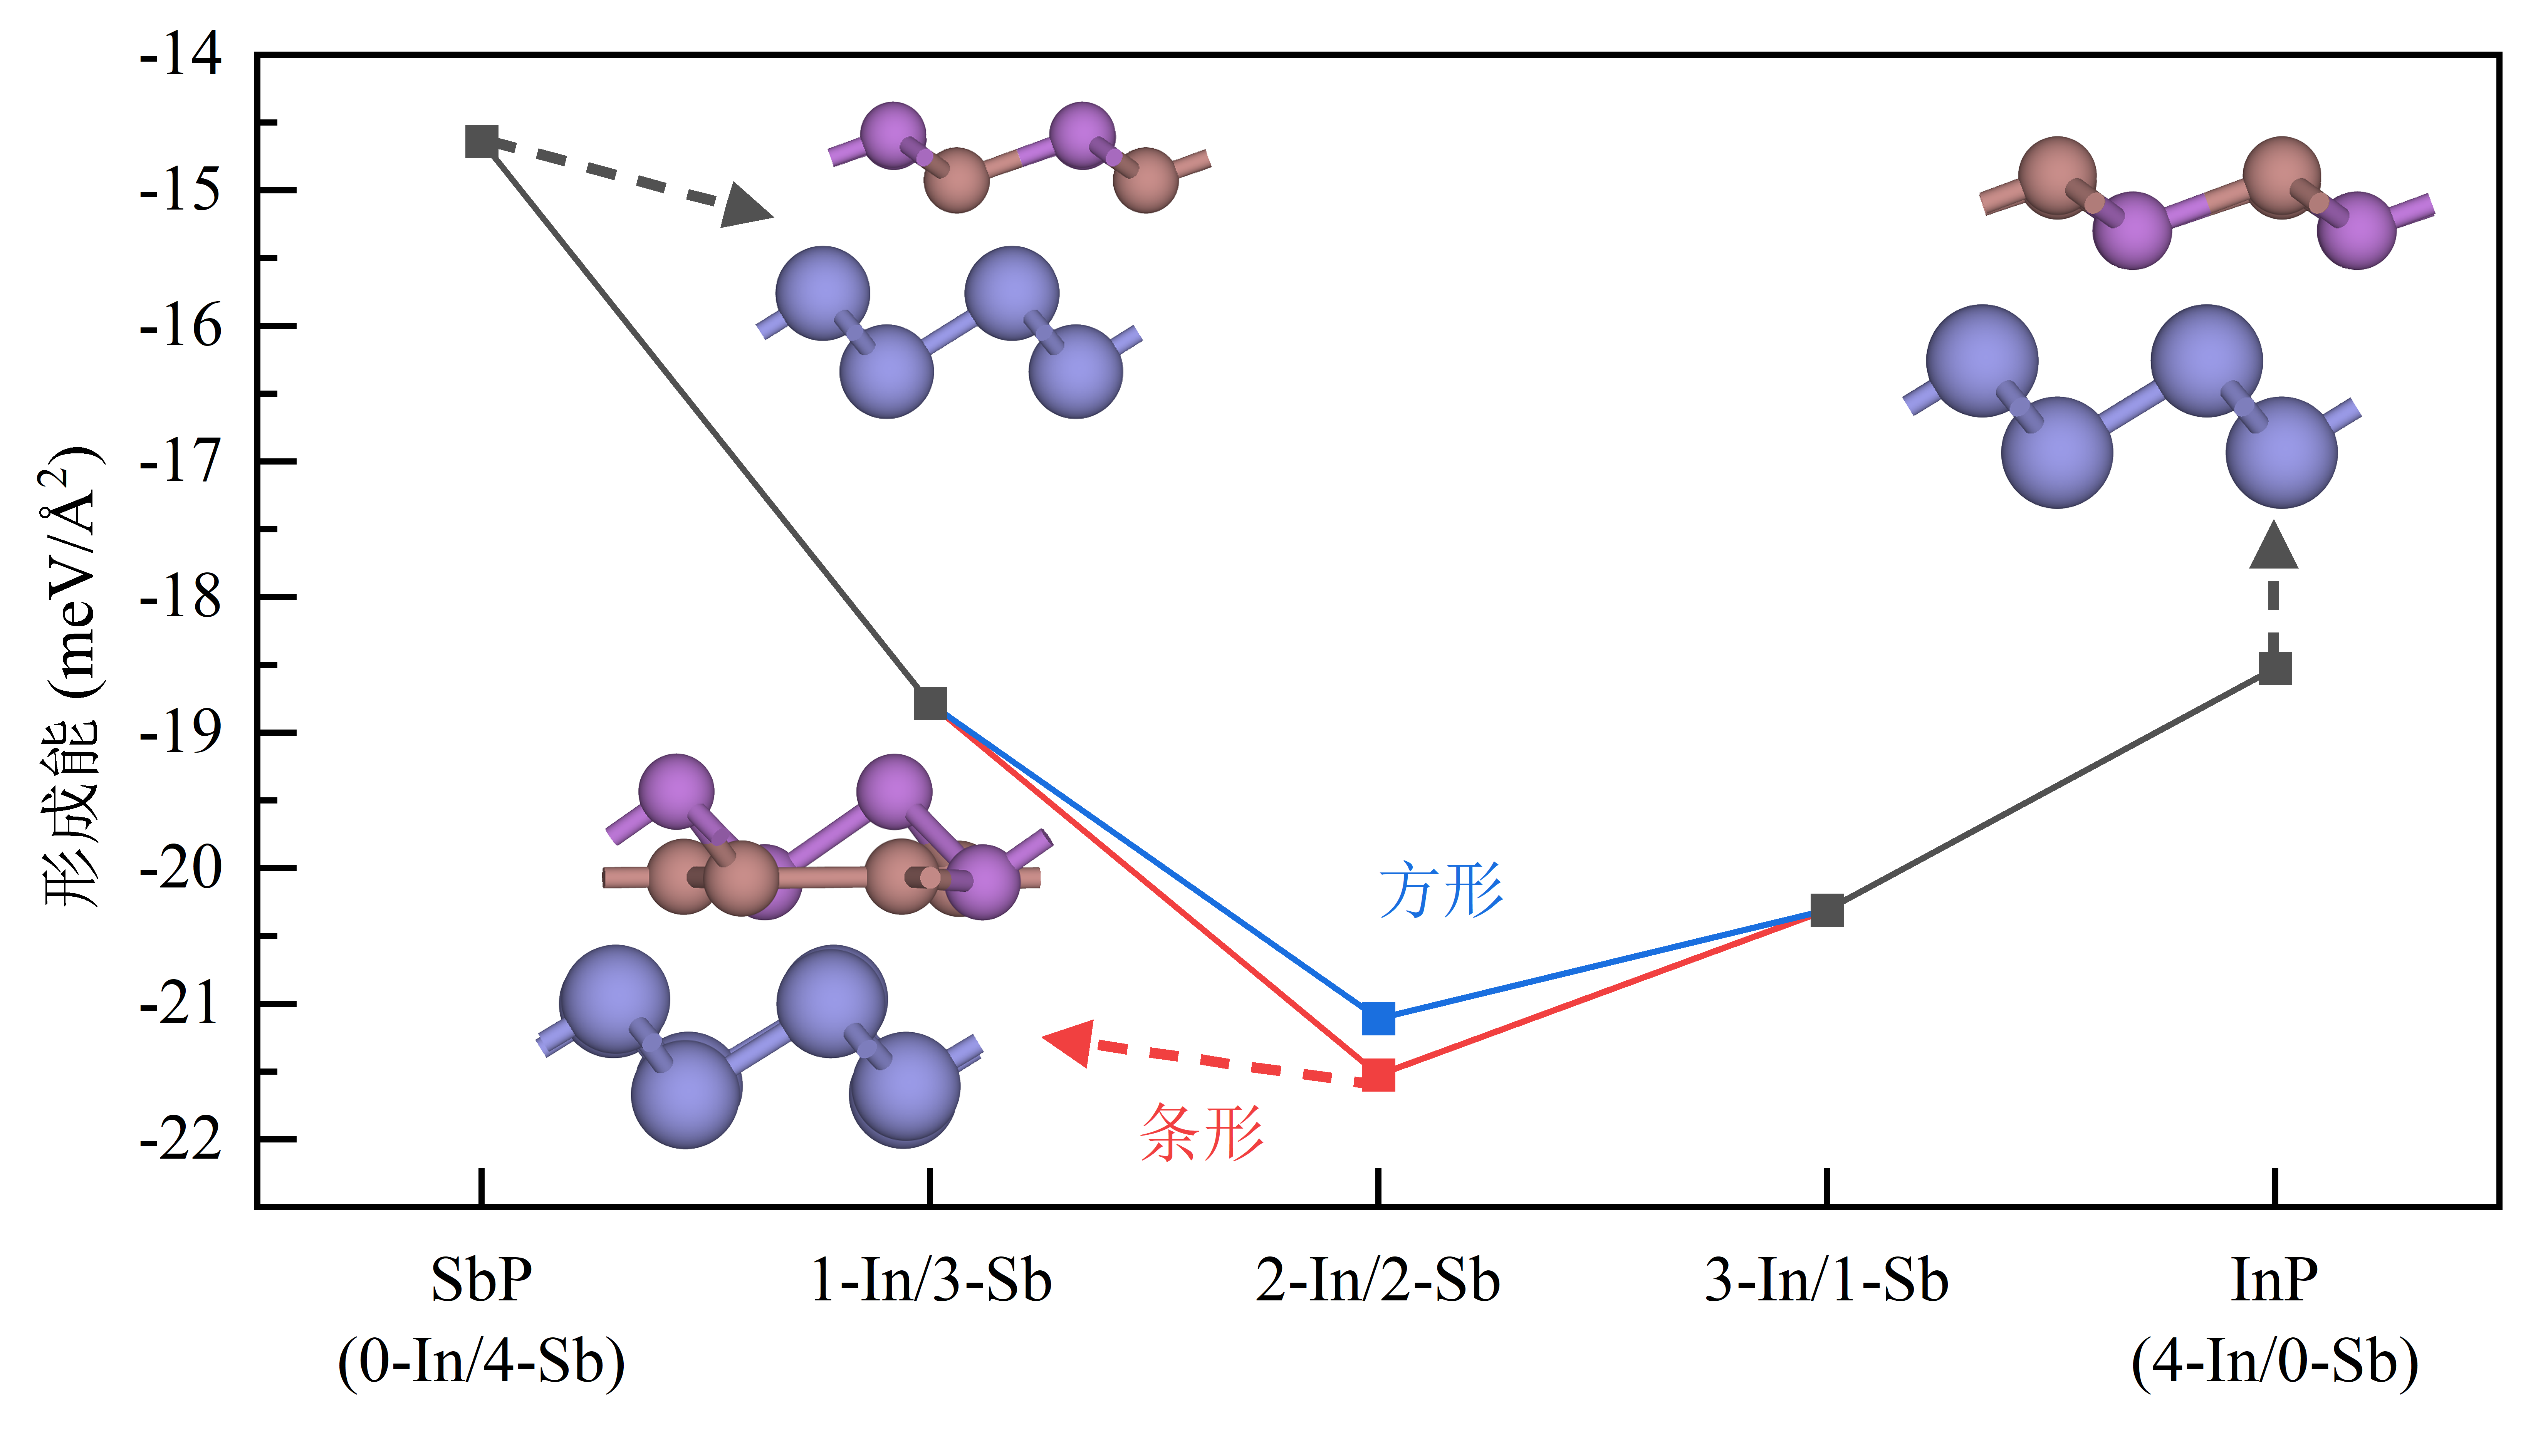
\includegraphics{pic/IS_DFT_1LInSb_all.png}
    \caption{\cemb{Bi(001)}衬底上不同极性单层\cemb{InSb}的形成能。}
    \label{fig:IS_DFT_1LInSb_all}
\end{figure}

在我们的进一步计算中,我们发现混合极性的单层\cemb{InSb(111)}构型(\InSbMLpolar{1}{3}、\InSbMLpolar{2}{2}以及\InSbMLpolar{3}{1})在形成能上更具有优势。从图\ref{fig:IS_DFT_1LInSb_all}上可以看出,混合极性中能量最低的\InSbMLpolar{1}{3}构型的形成能也略低于理想极性中更为稳定的\cemb{In}极性(\InSbMLpolar{4}{0})。因此,由于混合极性具有更高的能量稳定性,在生长的过程中\cemb{InSb}单层会倾向于由理想极性的结构(\cemb{Sb}极性和\cemb{In}极性)转变为混合极性。在4种混合极性中$\InSbMLpolar{2}{2}$结构的单层\cemb{InSb}的形成能最低。其中,$\InSbMLpolar{2}{2}$ 条形构型的形成能略低与$\InSbMLpolar{2}{2}$方形构型的形成能。这两形成能相近的$\InSbMLpolar{2}{2}$构型形成的能量最低态使得混合极性的\cemb{InSb}单层倾向于较为均匀的分布于这两个$\InSbMLpolar{2}{2}$构型之中,形成类似于非晶态的\cemb{InSb}单层。

利用分子动力学模拟方法,我们测试了$\InSbMLpolar{2}{2}$构型的热稳定性。如图\ref{fig:IS_structure_1Linsb_md}所示,我们选用形成能更低的$\InSbMLpolar{2}{2}$ 条形构型作为考察对象(图\ref{fig:IS_structure_1Linsb_md0ps}),模拟温度设为生长\cemb{InSb}常见的\SI{400}{\kelvin}。可能看到,在经过\SI{30}{\pico\second}的分子动力学模拟后。\cemb{InSb}单层的晶格结构被略微破坏,其中\cemb{In}的条状构型已经被热动能破坏,形成类似于菱形的结构,而\cemb{Sb}的条状构型保持较为完好。综合以上的计算结果,我们认为\cemb{InSb(111)}单层在\cemb{Sb(001)}衬底上由于热涨落的作用很可能无法保持在唯一的构型下,而是处于不同混合极性的热平衡态。在热平衡中,不同极性的\cemb{InSb}在热动能的驱动下相互转化,形成非晶态的单层\cemb{InSb}形貌。

\begin{figure}[!htb]
    \subfloat[]{
        \label{fig:IS_structure_1Linsb_md0ps}
        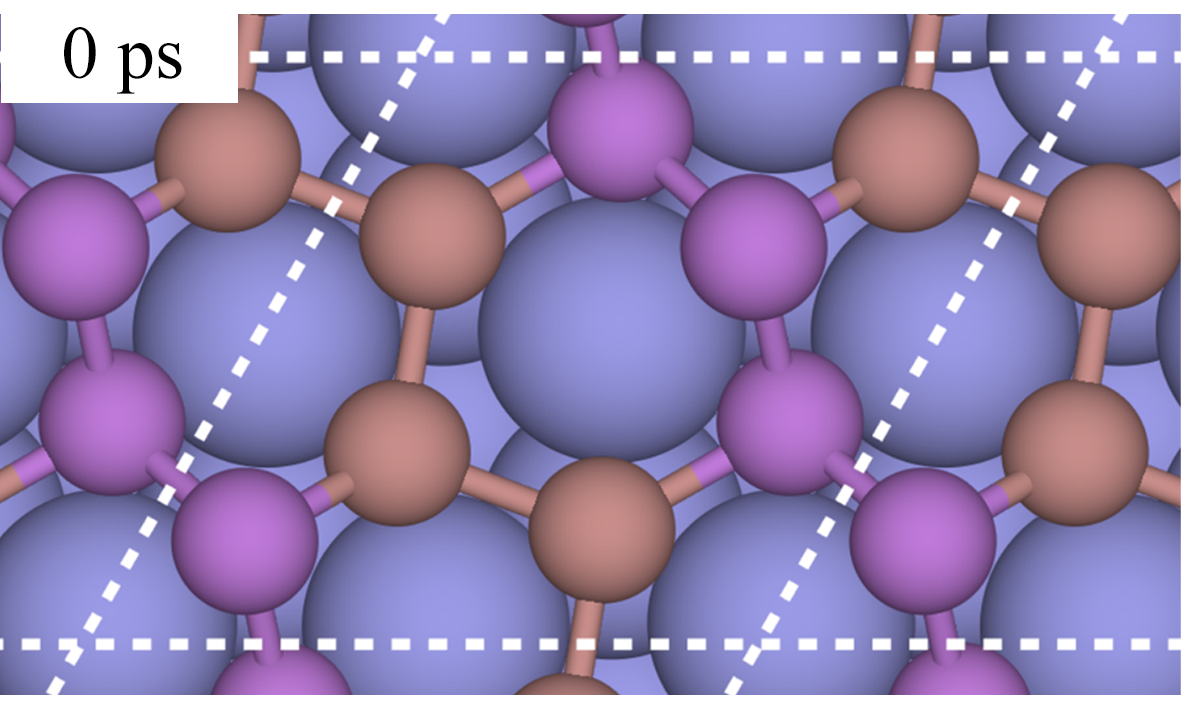
\includegraphics{pic/IS_structure_1Linsb_md0ps.png}
    }
    \subfloat[]{
        \label{fig:IS_structure_1Linsb_md10ps}
        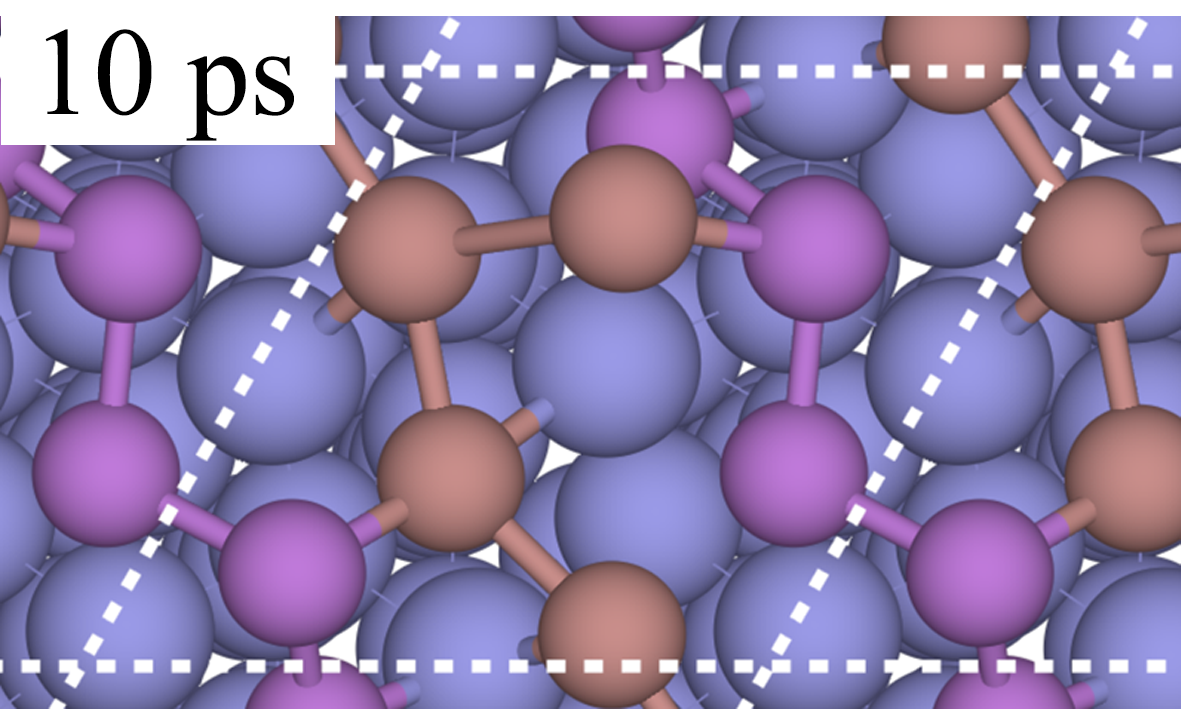
\includegraphics{pic/IS_structure_1Linsb_md10ps.png}
    }\\[-1ex]

    \subfloat[]{
        \label{fig:IS_structure_1Linsb_md20ps}
        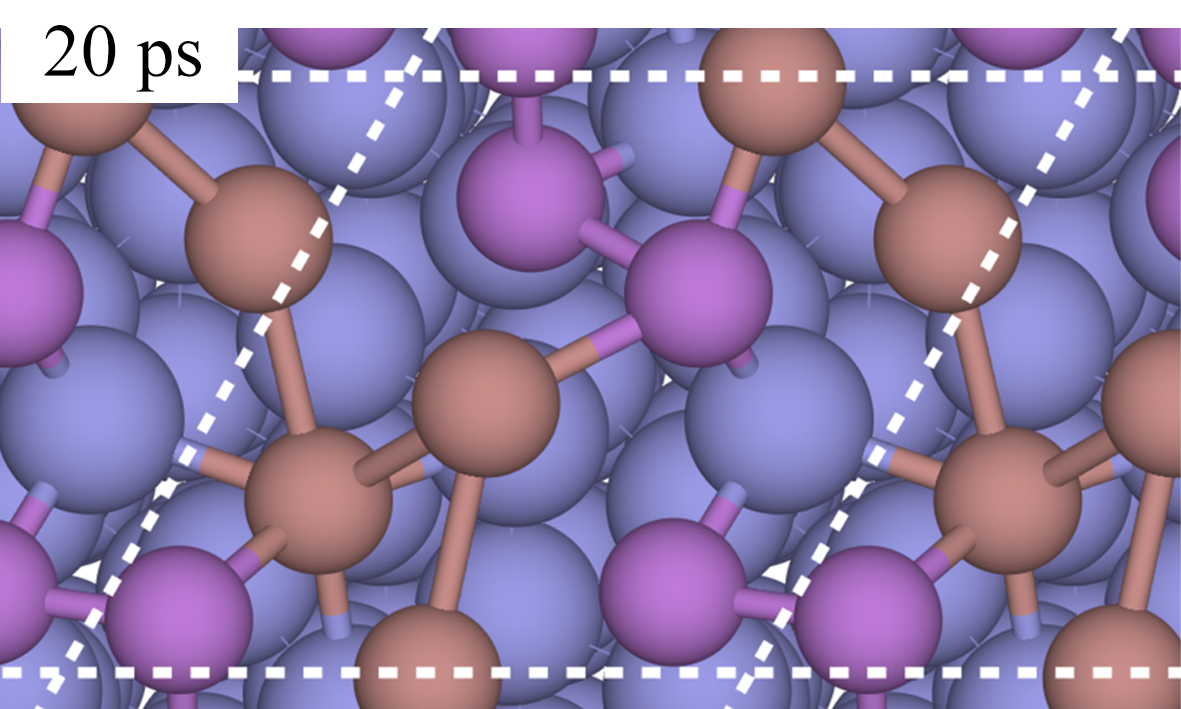
\includegraphics{pic/IS_structure_1Linsb_md20ps.png}
    }
    \subfloat[]{
        \label{fig:IS_structure_1Linsb_md30ps}
        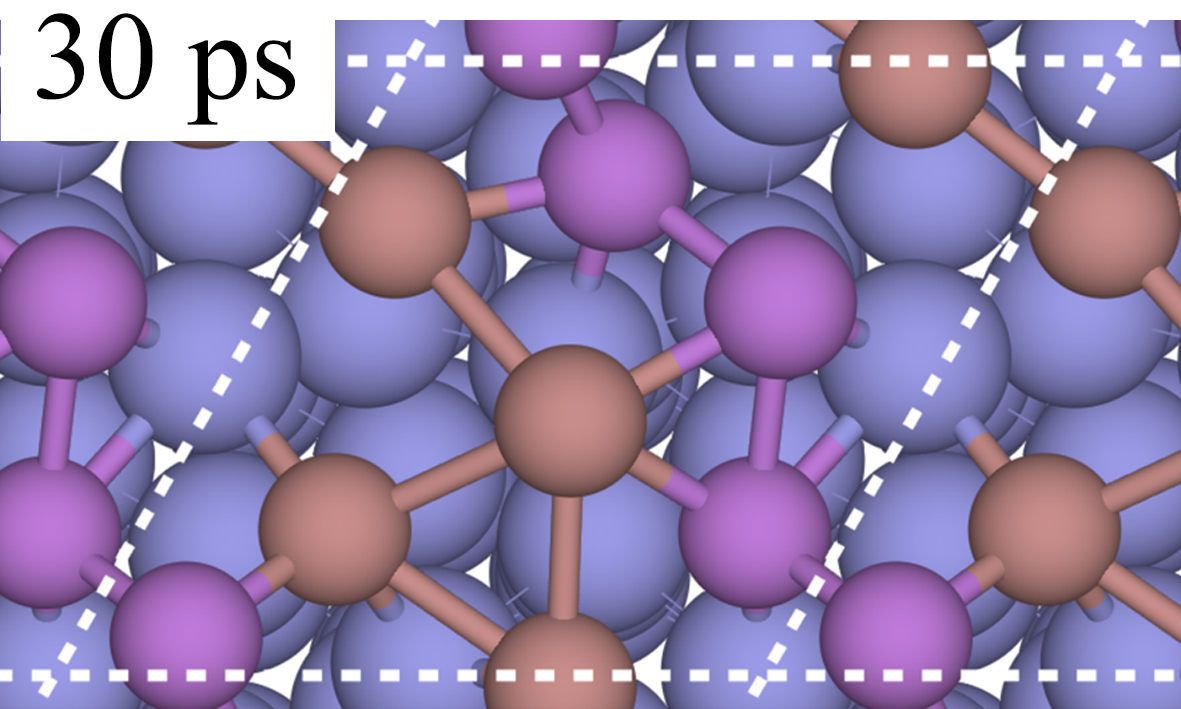
\includegraphics{pic/IS_structure_1Linsb_md30ps.png}
    }
    \caption{\cemb{Bi(001)}衬底上2-In/2-Sb条形极性\cemb{InSb}的分子动力学模拟结果。原子结构图中,\cemb{Bi}原子使用蓝色表示,\cemb{In}原子使用褐色表示,\cemb{Sb}原子使用紫色表示。}
    \label{fig:IS_structure_1Linsb_md}
\end{figure}

单层\cemb{InSb(111)}不同极性之间的转换能力我们通过将单层\cemb{InSb(111)}由一个极性的构型转变为另一个极性的构型所需的势垒进行判定。取\cemb{Sb}极性和\cemb{In}极性的的\cemb{InSb}单层之间的转换作为代表。这两个极性之间的转变涉及\cemb{InSb}单层内部所有的\cemb{In}原子和\cemb{Sb}原子,因此我们将其作为\cemb{InSb}极性转换势垒的上界。过渡态的计算结果如图\ref{fig:IS_DFT_1LInSb_InPtoSbPNeb}所示,从能量更高的\cemb{Sb}极性结构转变到\cemb{In}极性,单层\cemb{InSb}需要跨越约\SI{0.60}{\electronvolt}的势垒。根据统计力学原理\citing{RN945-1935},单层\cemb{InSb}从\cemb{Sb}极性转变到\cemb{In}极性的频率$r$为\chinesecolon
\[
    r=e^{\frac{-\energyVar{a}{}}{\kbconst T}}e^{\frac{\Delta S}{\kbconst}} \frac{\kbconst T}{h}
\]

其中,$\energyVar{a}{}$为反应的激活能,$\kbconst$为玻尔兹曼常数,$T$为温度,$h$为普朗克常数,$\Delta S$为反应过程中初态和过渡态之间的熵变,我们使用密度泛函理论计算结合原子震动能谱分析进行计算。在\SI{400}{\kelvin}的温度下,单层\cemb{InSb}从\cemb{Sb}极性转变到\cemb{In}极性的频率$r$约为\SI{3e5}{\per\second},证明了在\cemb{Bi(001)}衬底表面,\cemb{InSb}单层具有较高的极性转变能力。

\begin{figure}[!htb]
    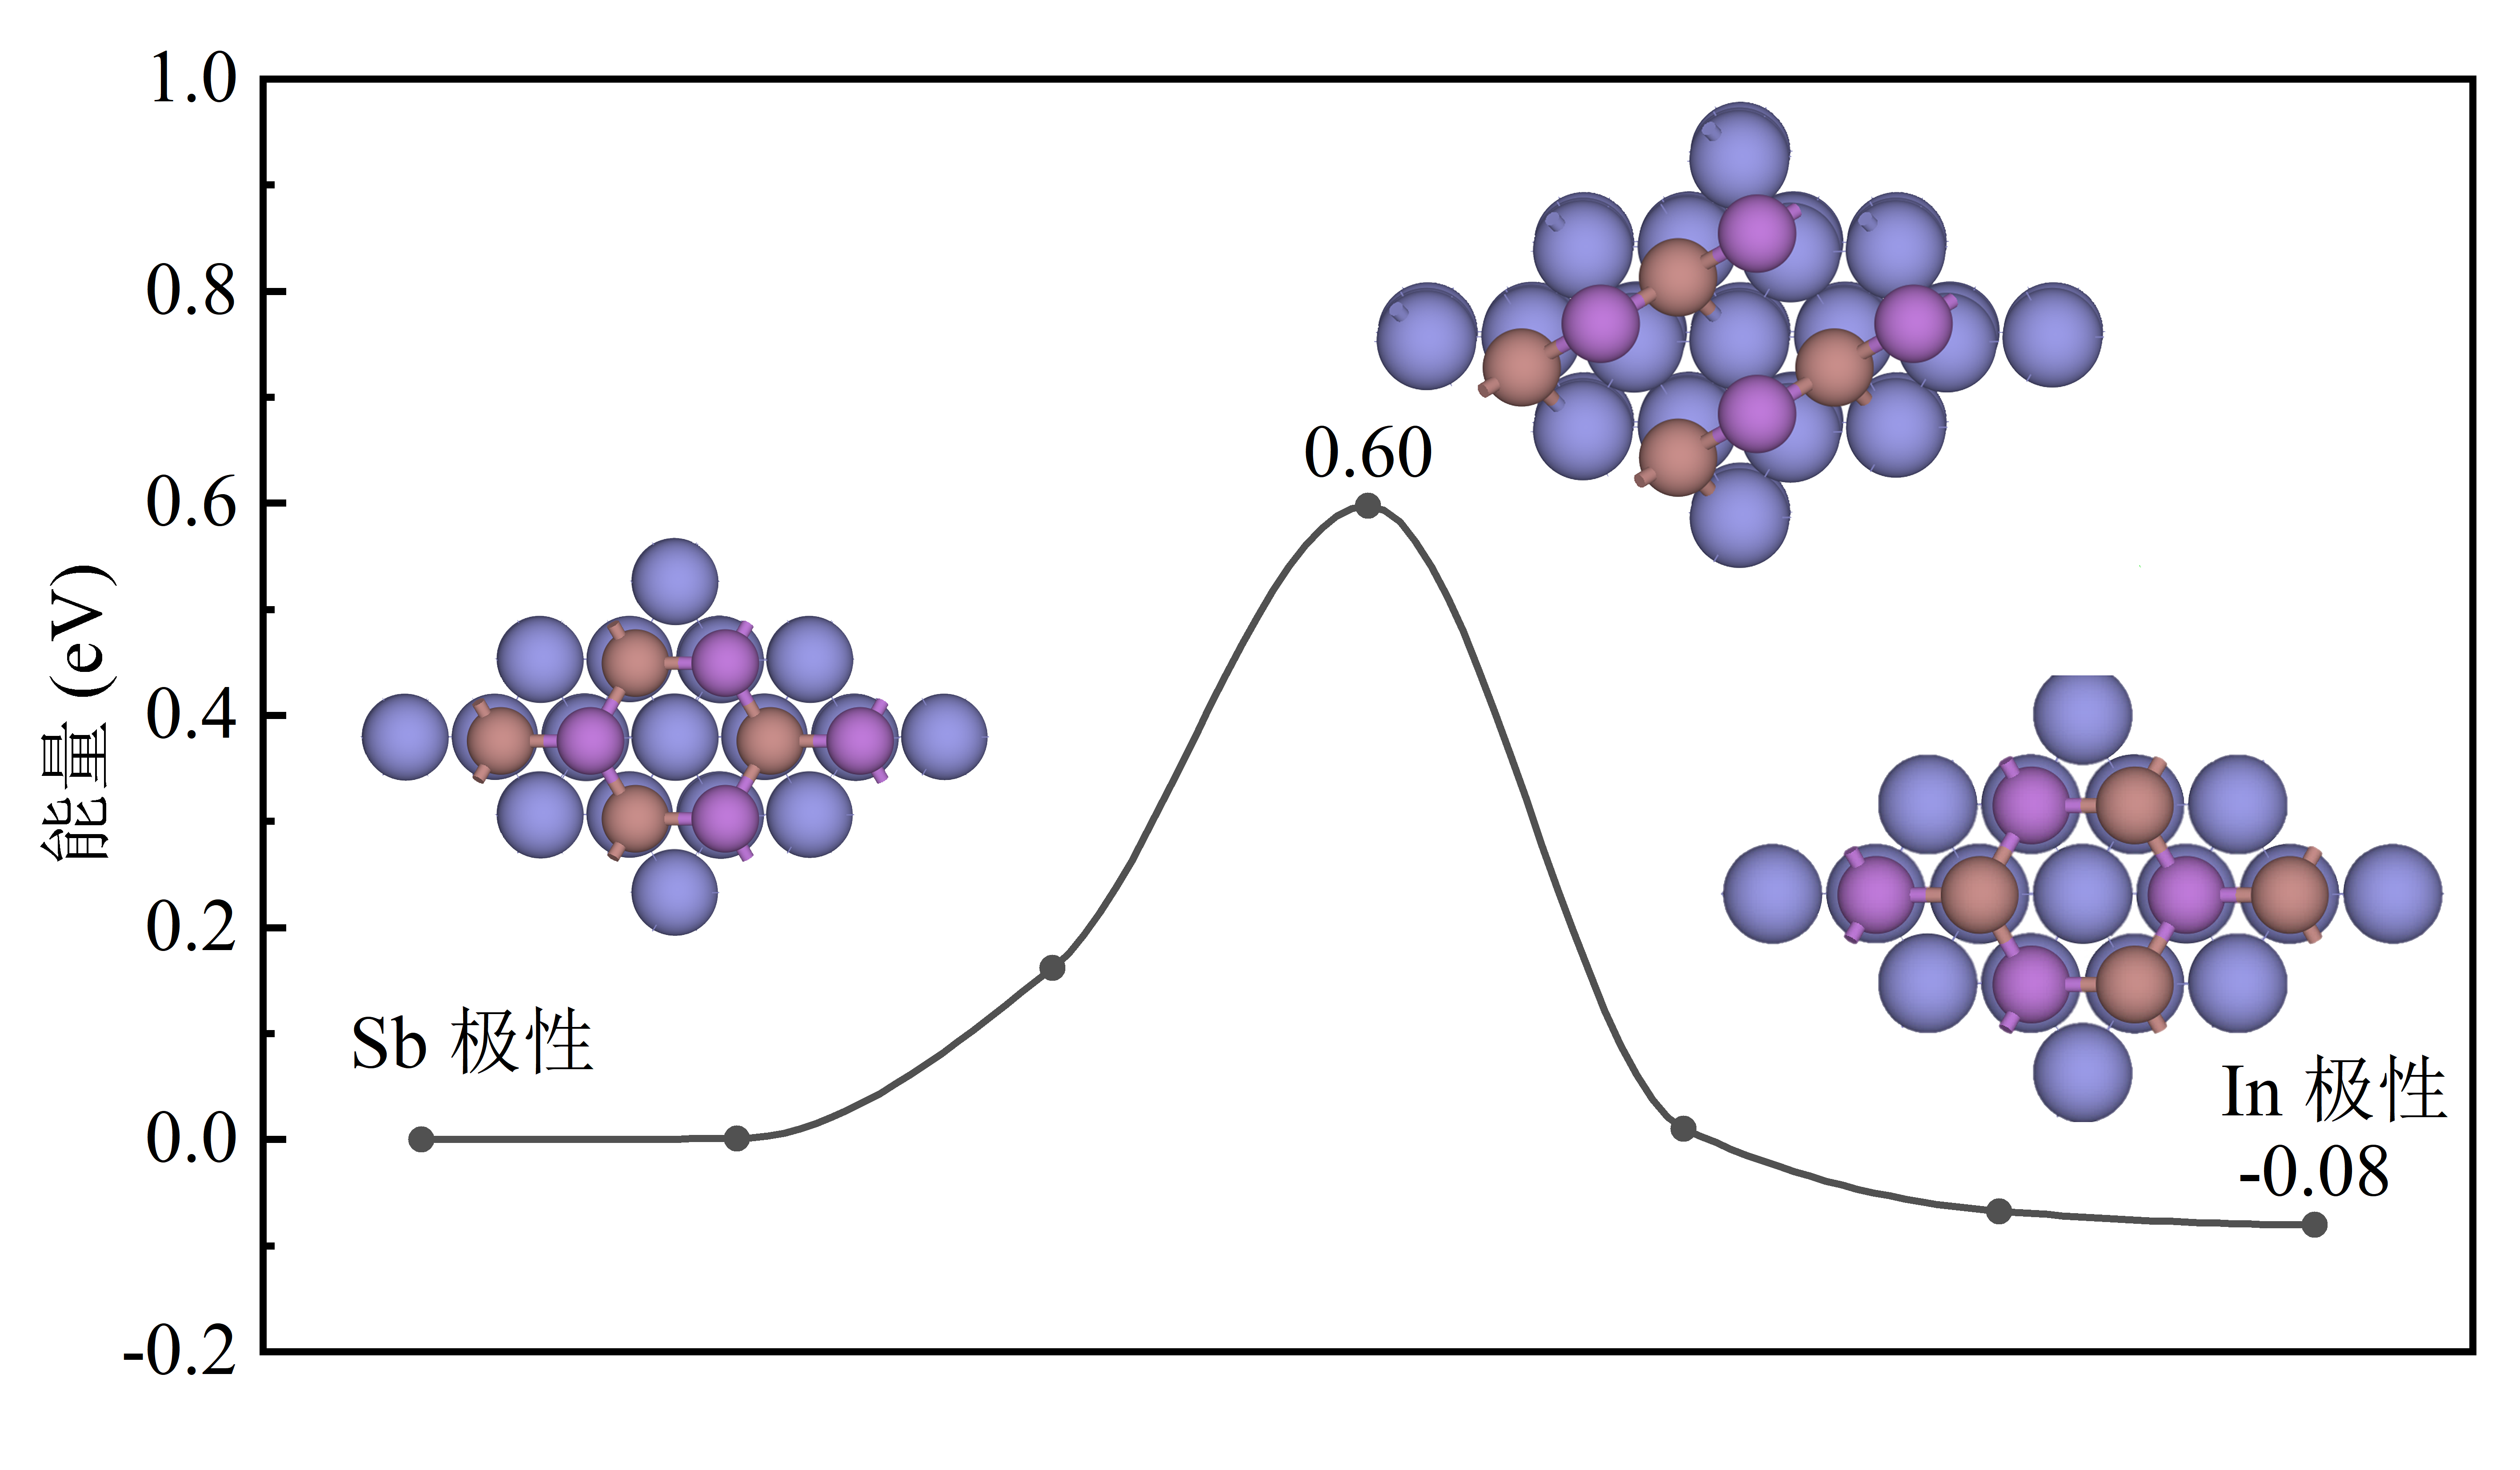
\includegraphics{pic/IS_DFT_1InSb_flipBarrier.png}
    \caption{\cemb{Bi(001)}衬底上单层\cemb{InSb}的极性转换势垒。原子结构图中,\cemb{Bi}原子使用蓝色表示,\cemb{In}原子使用褐色表示,\cemb{Sb}原子使用紫色表示。}
    \label{fig:IS_DFT_1LInSb_InPtoSbPNeb}
\end{figure}

\section{双层锑化铟的生长机理}
在上一节中,我们通过理论计算表明了单层的\cemb{InS(111)}以$\InSbMLpolar{2}{2}$极性为主,多种极性热平衡混合的构型存在于\cemb{Bi(001)}衬底的表面。我们将第二层\cemb{InSb(001)}放置在单层\cemb{InSb}上方,研究双层\cemb{InSb(111)}在\cemb{Bi(001)}衬底上的生长机理和极性演化情况。

\subsection{双层锑化铟的生长过程}
对于双层\cemb{InSb}在\cemb{Bi(001)}衬底上的生长,我们首先探究第二层\cemb{InSb(111)}对于\cemb{InSb}极性的影响。对于第二层\cemb{InSb(111)},我们选用对应的表面重构构型进行代表。根据先前的研究\citing{RN915-1998, RN896-1998},在\cemb{InSb(111)}的表面由于极性的不同会形成两种不同的表面重构,一种是对应于\cemb{Sb}极性的\cemb{Sb}三聚体(\cemb{Sb} trimer)表面重构,另一种是对应于\cemb{In}极性的\cemb{In}空位(\cemb{In} vacancy)表面重构。

如图\ref{fig:IS_structure_2Linsb}所示,我们考虑不同表面重构的\cemb{InSb}第二层和不同极性的\cemb{InSb}第一层的所有组合进行形成能计算。以\cemb{In}极性的\cemb{InSb}第一层为代表,我们在图\ref{fig:IS_structure_2Linsb_SbT40}和图\ref{fig:IS_structure_2Linsb_InV40}中绘制了优化后的双层\cemb{InSb}的原子结构。可以看到对于\cemb{Sb}三聚体的第二层能够与\cemb{In}极性的第一层的上表面\cemb{In}原子产生相互作用,略微提高于其相接触的\cemb{In}原子的相对高度。对于\cemb{In} 空位的第二层,其在\cemb{In}极性的第一层\cemb{InSb}上方呈现出平面化的形貌。\cemb{In}空位重构中四个\cemb{Sb}原子与第一层上表面的\cemb{In}原子产生作用。

\begin{figure}[!htb]
    \subfloat[]{
        \label{fig:IS_2LInSb_config}
        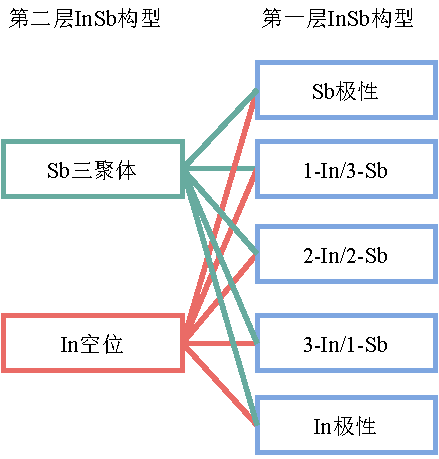
\includegraphics[width=0.48\textwidth]{pic/IS_2LInSb_config.pdf}
    }
    \begin{minipage}[b]{0.5\textwidth}
        \subfloat[]{
            \label{fig:IS_structure_2Linsb_SbT40}
            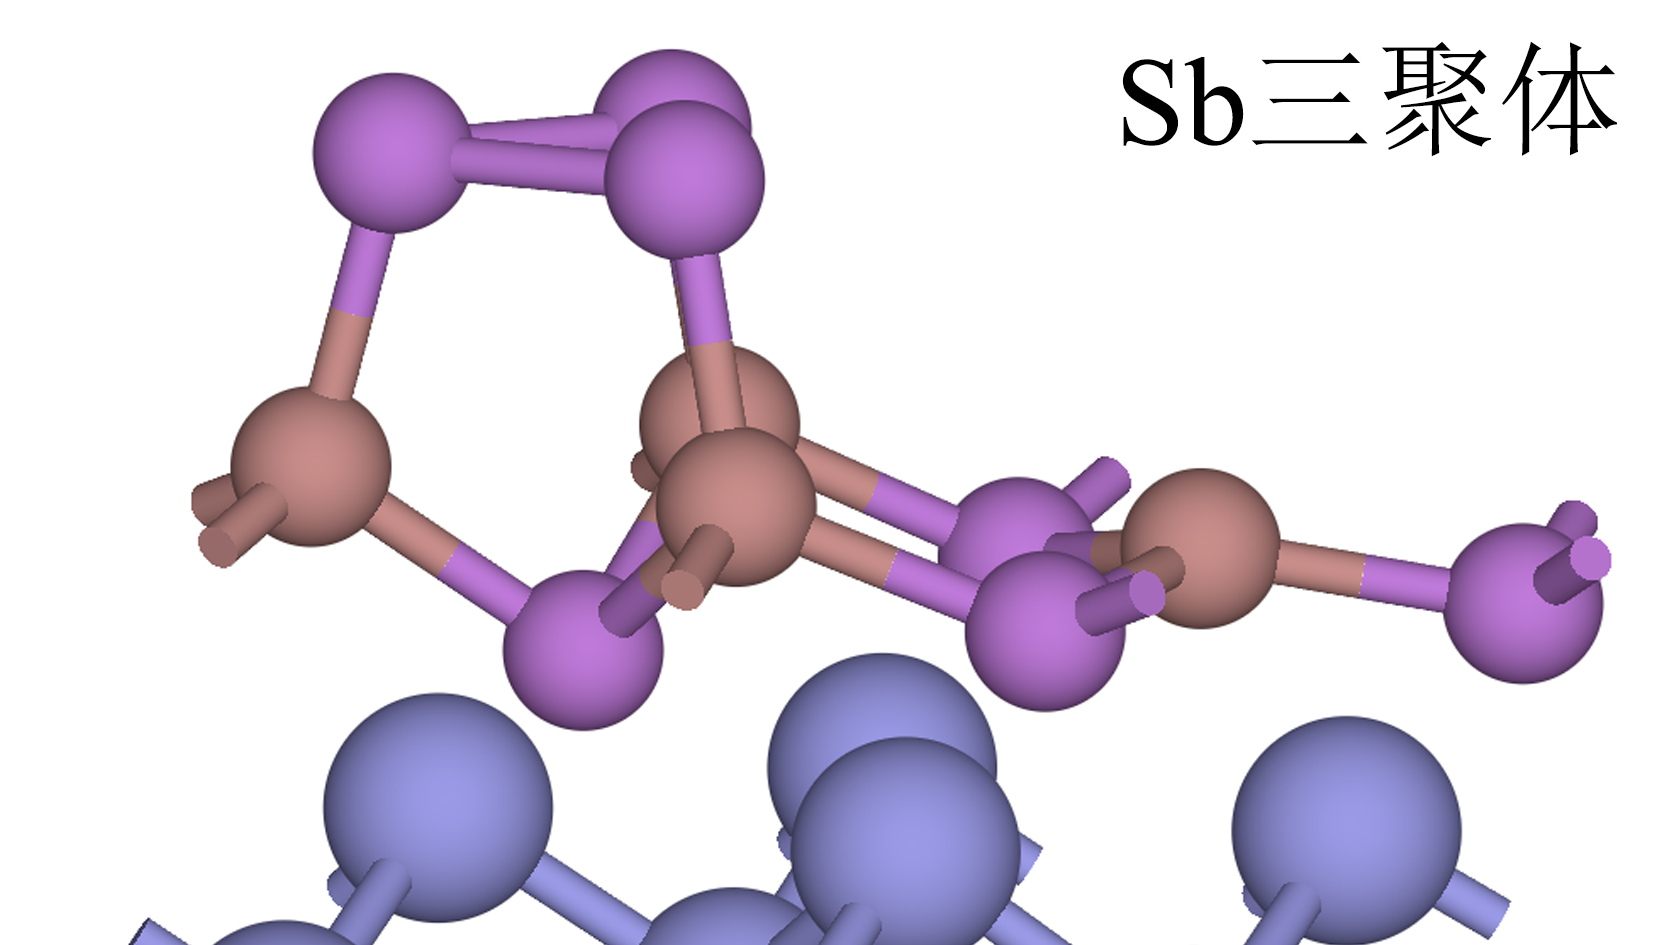
\includegraphics[width=0.8\textwidth]{pic/IS_structure_2Linsb_SbT-40_3Dview.png}
        }
        \newline
        \subfloat[]{
            \label{fig:IS_structure_2Linsb_InV40}
            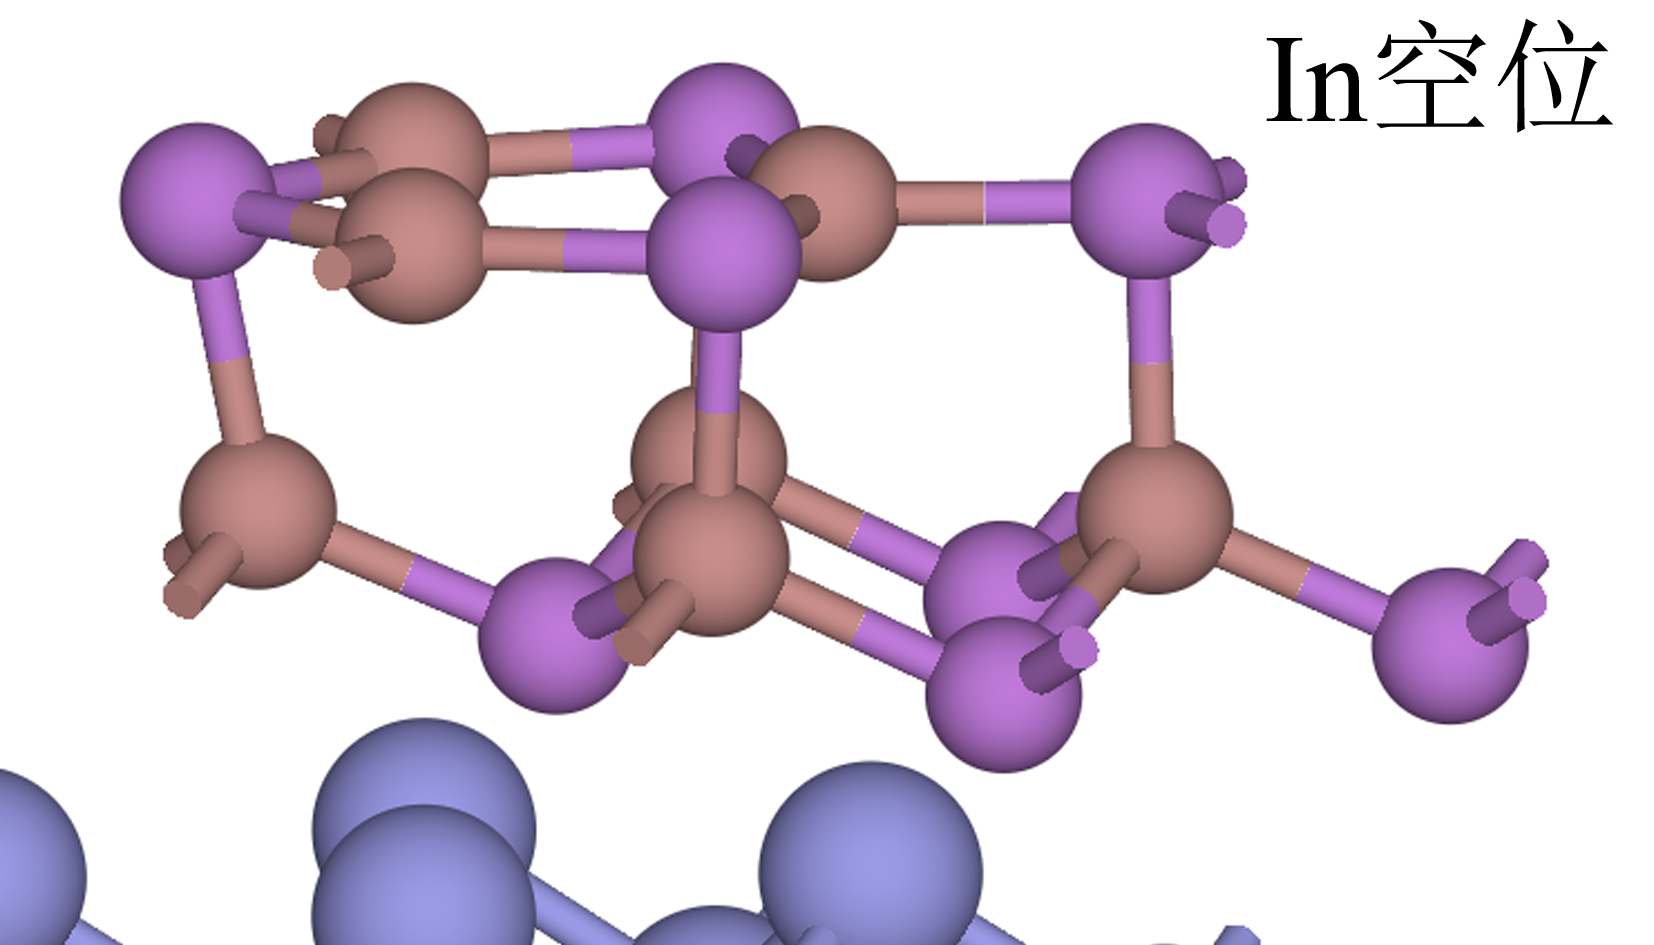
\includegraphics[width=0.8\textwidth]{pic/IS_structure_2Linsb_InV-40_3Dview.png}
        }
    \end{minipage}
    \caption{双层\cemb{InSb}极性极性组合图及原子结构示意图。(a)双层\cemb{InSb}极性极性组合示意图;(b)双层\cemb{InSb}原子结构,\cemb{Sb}三聚体第二层覆盖\cemb{In}极性第一层;(b)双层\cemb{InSb}原子结构,\cemb{In}空位第二层覆盖\cemb{In}极性第一层。原子结构图中,\cemb{Bi}原子使用蓝色表示,\cemb{In}原子使用褐色表示,\cemb{Sb}原子使用紫色表示。}
    \label{fig:IS_structure_2Linsb}
\end{figure}

在图\ref{fig:IS_DFT_2LInSb_formationEnergy}中,我们绘制了\cemb{Bi(001)}衬底上具有不同极性第一层\cemb{InSb}的双层\cemb{InSb}的形成能分布。先前的研究表明,不同的前驱体比例会对生长形貌产生极大的影响\citing{RN935-2002, RN398-2002}。因此同\cemb{In}和\cemb{Sb}原子的吸附机制研究一致,我们引入\cemb{In}原子的化学势$\muVar{In}{}$代表生长环境中$\cemb{In}:\cemb{Sb}$比的变化。为了绘图清晰,我们在图\ref{fig:IS_DFT_2LInSb_formationEnergy}只绘制了不同构型在纯\cemb{Sb}环境和纯\cemb{In}环境两个极限下的形成能取值。由于在\cemb{Sb}三聚体重构和\cemb{In}空位重构中,均为\cemb{Sb}原子的数量占有,因此根据式\ref{eq:IS_formationEnenrgy}和式\ref{eq:IS_bulkEqmb},以\cemb{Sb}三聚体重构和\cemb{In}空位重构为第二层的双层\cemb{InSb}的形成能均会随着\cemb{In}原子化学式$\muVar{In}{}$的上升(接近纯\cemb{In}环境)而上升。

\begin{figure}[!htb]
    \subfloat[]{
        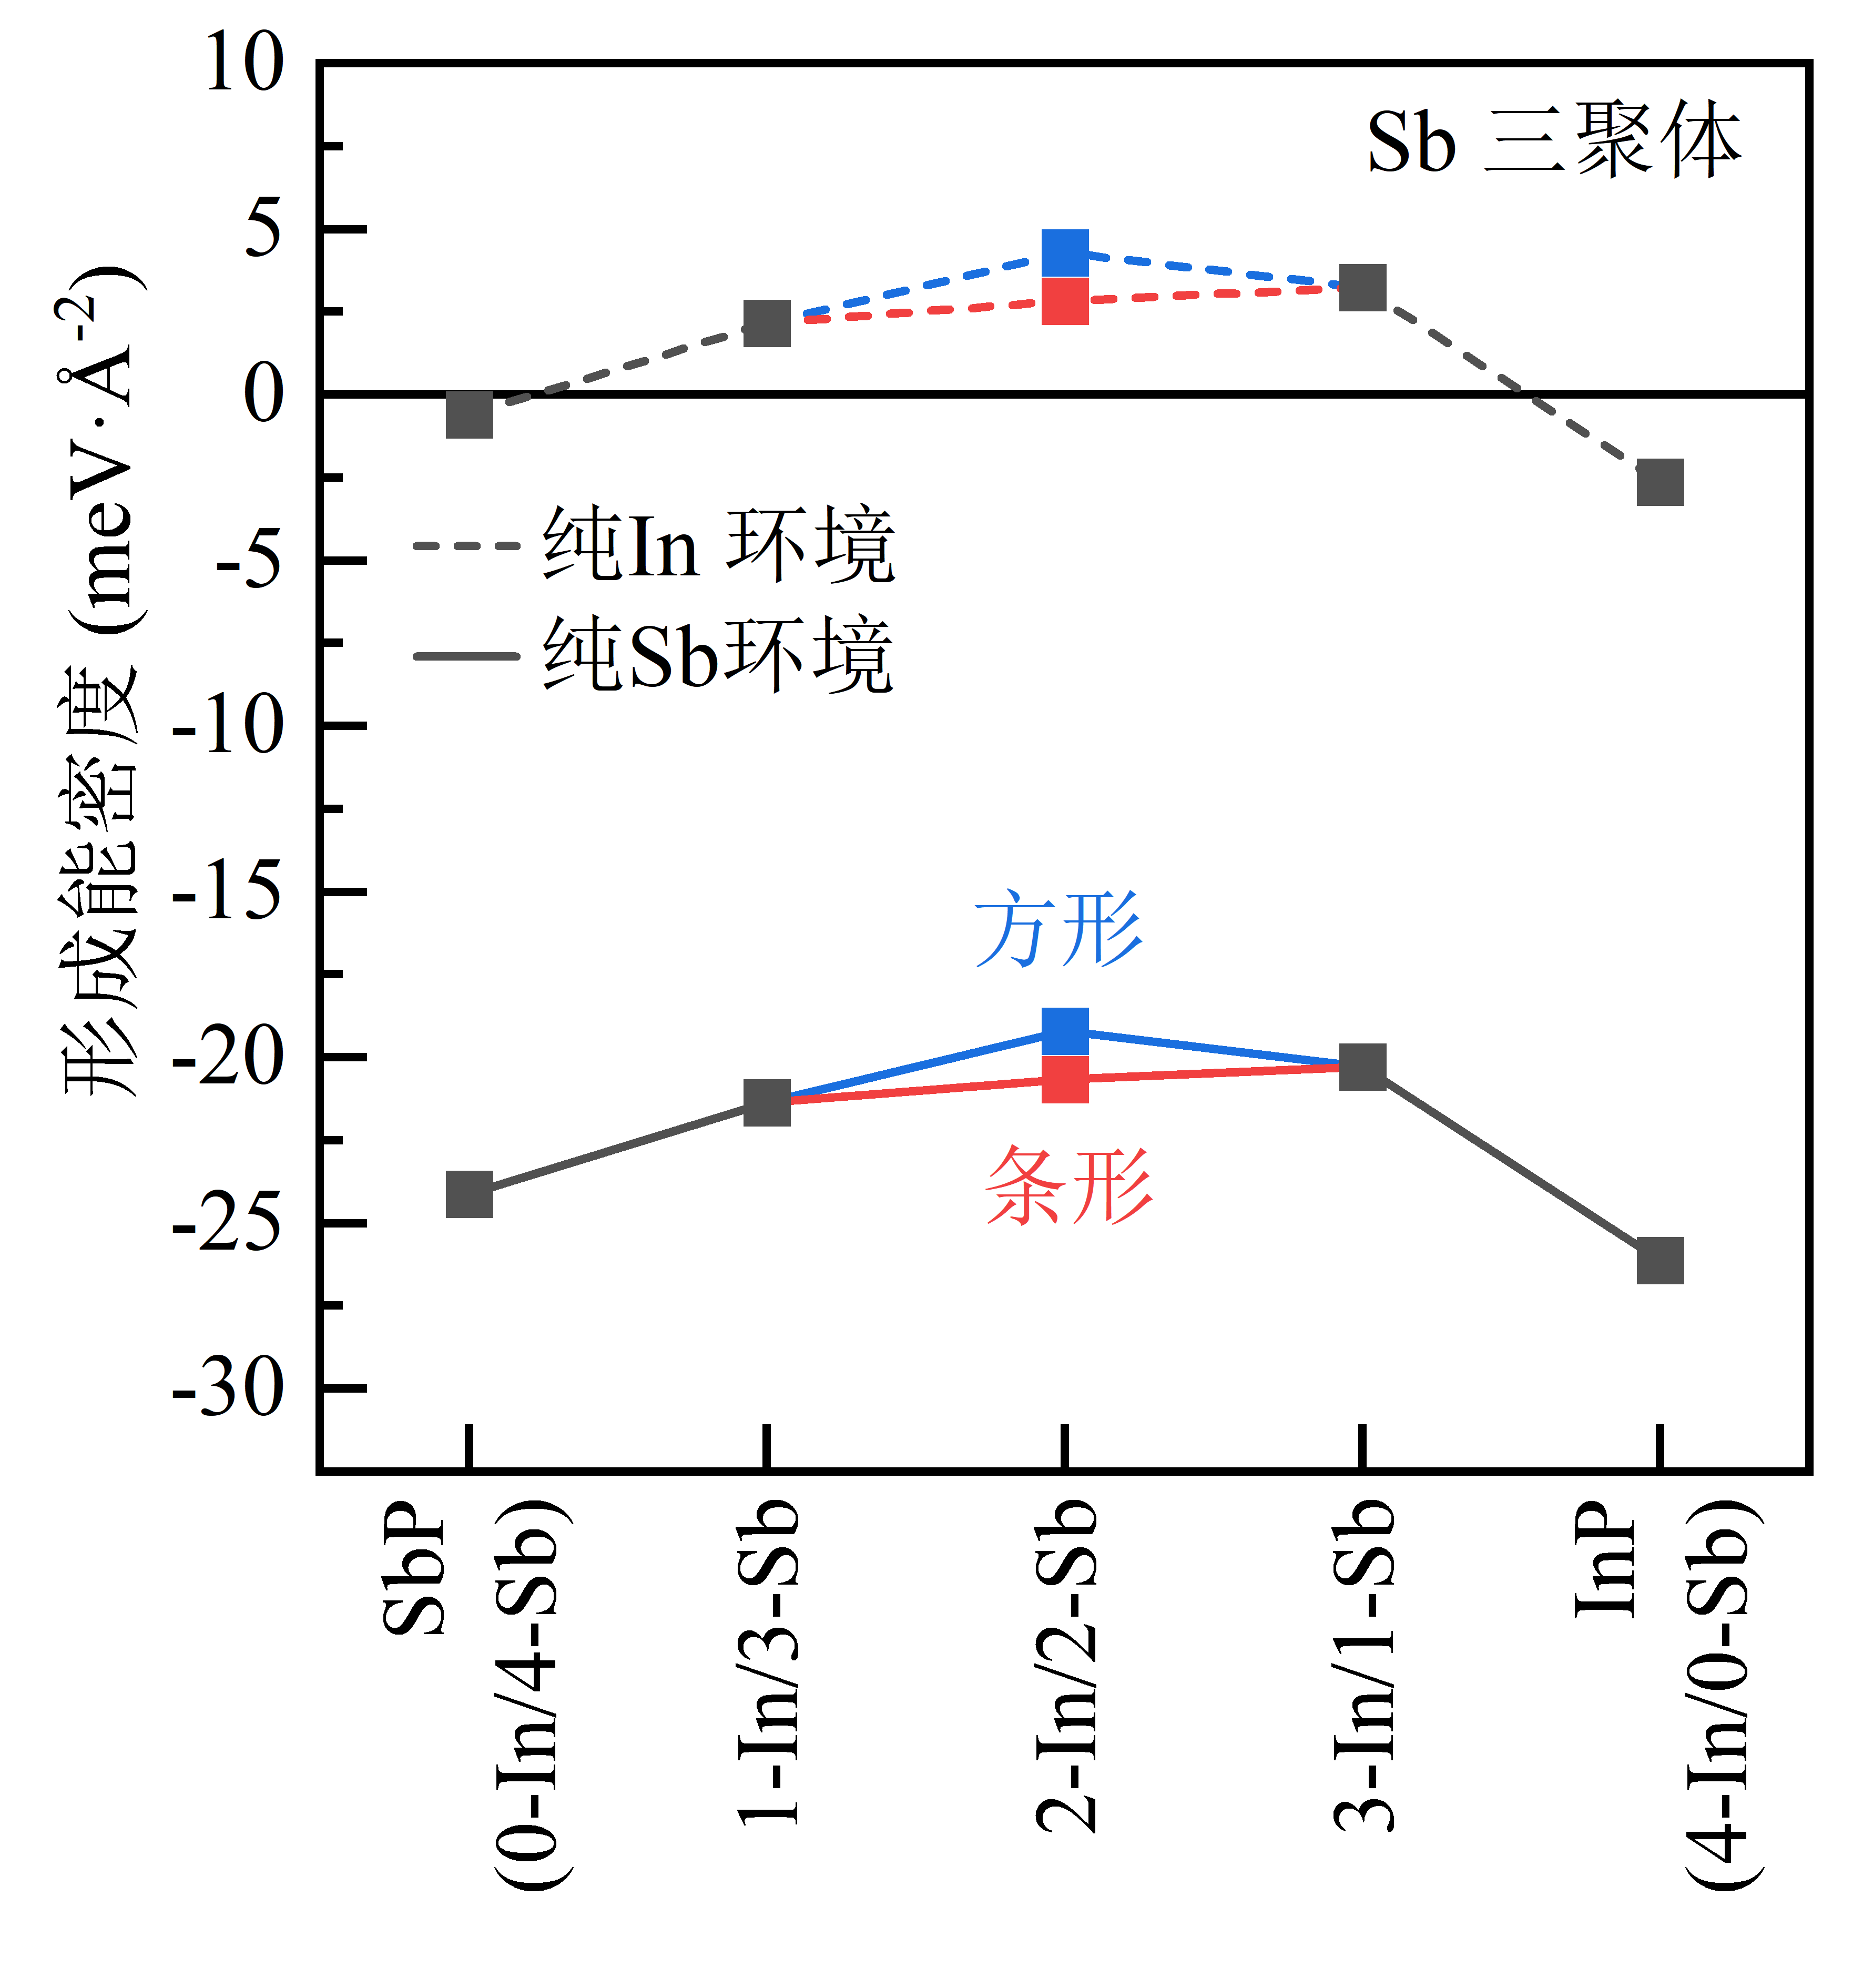
\includegraphics[width=0.45\textwidth]{pic/IS_DFT_2LInSb_SbTonAll.png}
        \label{fig:IS_DFT_2LInSb_SbTonAll}
    }
    \subfloat[]{
        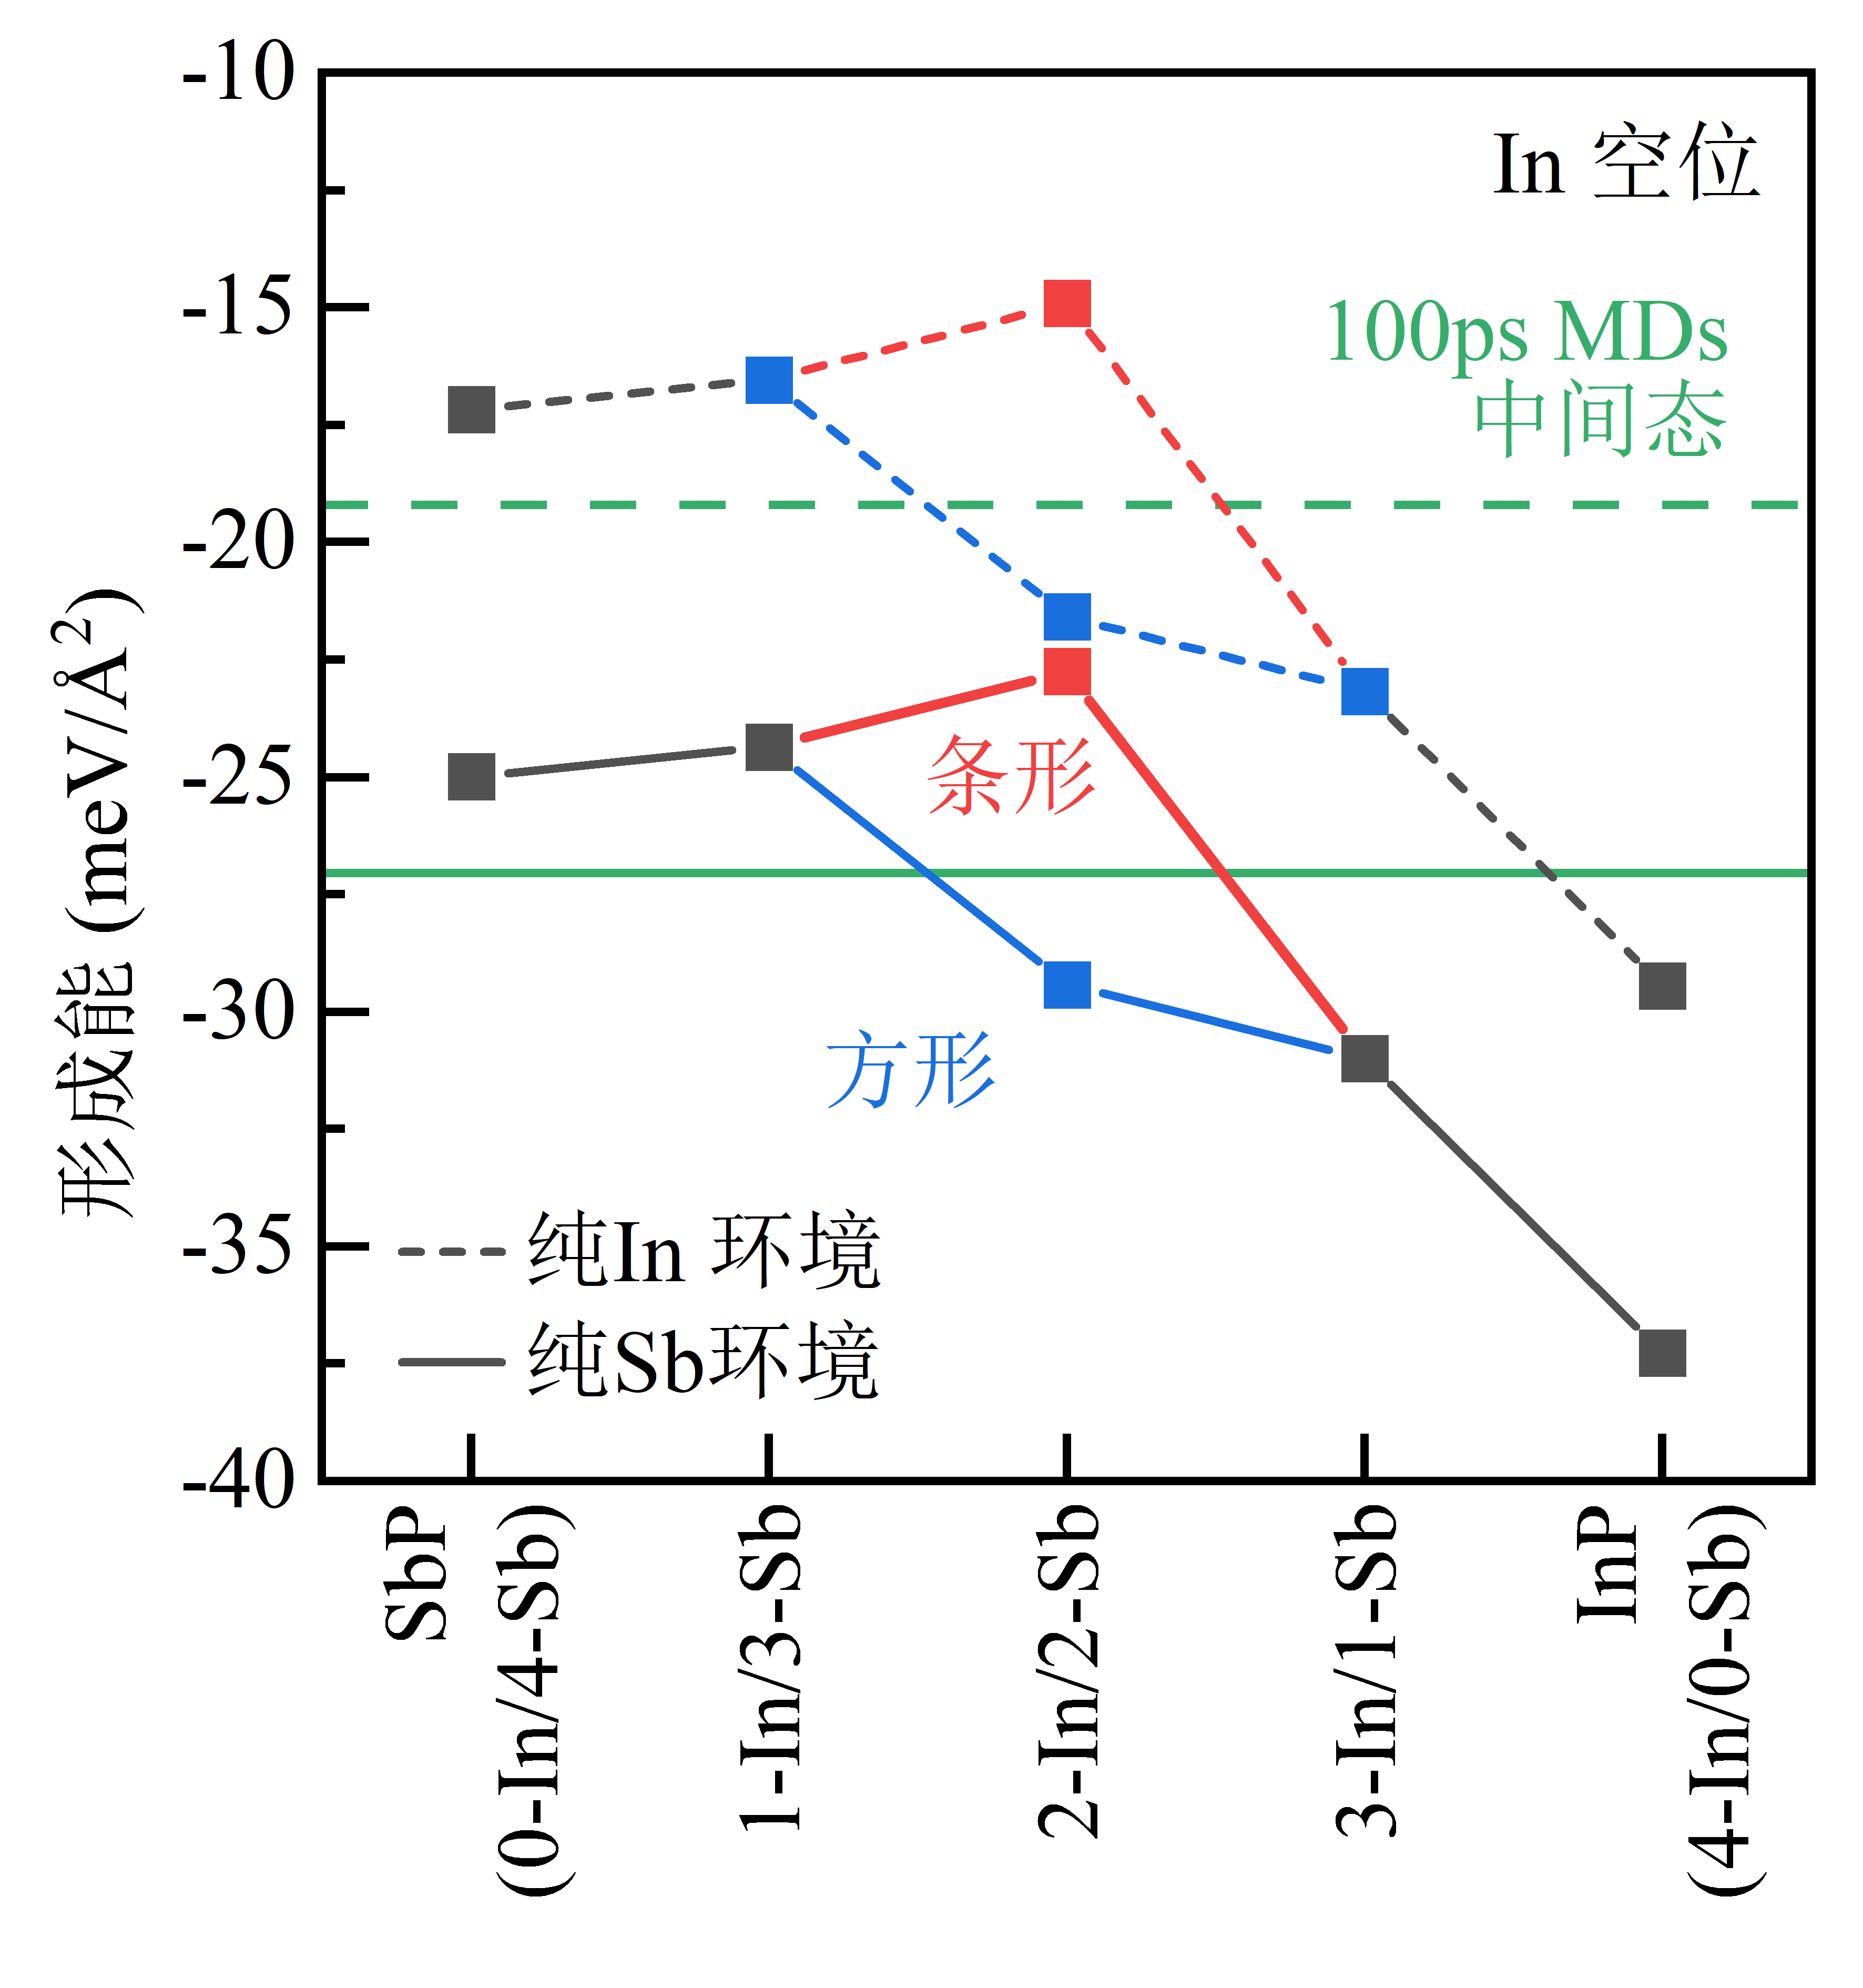
\includegraphics[width=0.45\textwidth]{pic/IS_DFT_2LInSb_InVonAll.png}
        \label{fig:IS_DFT_2LInSb_InVonAll}
    }
    \caption{\cemb{Bi(001)}衬底上双层\cemb{InSb}的形成能分布。(a)以Sb三聚体为第二层的双层\cemb{InSb}的形成能分布;(b)以In空位层为第二层的双层\cemb{InSb}的形成能分布。}
    \label{fig:IS_DFT_2LInSb_formationEnergy}
\end{figure}

当第二层为\cemb{Sb}三聚体重构时,第一层为理想极化结构(\cemb{Sb}极性和\cemb{In}极性)的双层\cemb{InSb}相比于第一层为混合极化结构的双层\cemb{InSb}拥有更低的形成能。理想极化的第一层\cemb{InSb}在形成能分布中作为两个极小值点,吸引其他拥有混合极性第一层的双层\cemb{InSb}向理想极化转变。使得原本在非静态单层中以混合极性为主的平衡态分化成为\cemb{Sb}极性和\cemb{In}极性共存的多晶态。同时,当生长环境中的接近纯\cemb{In}极限时,第一层为混合极性的双层\cemb{InSb}的形成能大于零而第一层为理想极性的双层\cemb{InSb}的形成能保持在小于零的状态。在这种情况下,由于较高的\cemb{In}原子活性,可能会导致第一层为混合极性的双层\cemb{InSb}分解,进一步加速了双层\cemb{InSb}向理想极性的第一层构型转化。

当第二层为\cemb{In}空位重构时,\cemb{In}空位层和作为第一层的\cemb{Sb}极性\cemb{InSb}之间的作用没有\cemb{Sb}三聚体作为第二层时的那么强烈。\cemb{In}空位重构的第二层无法\cemb{Sb}极性的第一层的形成能降低到混合极性之下。导致了第二层为\cemb{In}空位重构时,在双层\cemb{InSb}中只有第一层为\cemb{In}极性时为最小能量态。在\cemb{In}空位重构下,\cemb{Sb}极性的第一层只需要跨越\SI{0.63}{\mievpas}的能量台阶(\InSbMLpolar{1}{3})即可一步步翻转至\cemb{In}极性的第一层,其中的过程均为放热反应。在这种情况下,我们认为当第二层为\cemb{In}空位重构时,极性为混合极性或者\cemb{Sb}极性的第一层会逐渐极化至\cemb{In}极性。

在图\ref{fig:IS_DFT_2LInSb_formationEnergy}中,形成能的计算显示在生长了第二层\cemb{InSb}后,重构的第二层\cemb{InSb}会使得第一层已生长的非晶态\cemb{InSb}趋向于转变为多晶的形态(第二层为\cemb{Sb}三聚体重构)或者\cemb{In}极性的形态(第二层为\cemb{In}空位重构)。

为了探究在双层\cemb{InSb}中第一层\cemb{InSb}由非晶态向单一\cemb{In}极性转变的动力学过程,我们以\cemb{In}空位作为第二层,$\InSbMLpolar{2}{2}$条形构型作为第一层组成的双层\cemb{InSb}作为研究对象,在\cemb{Bi}衬底上进行分子动力学模拟。如图\ref{fig:IS_structure_2Linsb_md50ps}所示,在经过了\SI{50}{\pico\second}的分子动力学模拟后,可以看到第一层的$\InSbMLpolar{2}{2}$构型已经完全被破坏。有一个原属于第一层的\cemb{Sb}原子越过一二层\cemb{InSb}的界面,被挤入了第二层。同时,第一层的\cemb{InSb}由于缺少了一个\cemb{Sb}原子,原本晶格中的褶皱变得扁平。随着分子动力学模拟的继续,第一个\cemb{In}极性的次表面出现在模拟开始约\SI{60}{\pico\second}的时候(图\ref{fig:IS_structure_2Linsb_md60ps})。这个次表面是一个位于顶点的\cemb{In}原子和三个位于底部的\cemb{Sb}原子组成的四面体结构,并且在我们的模拟过程中一直维持到了\SI{100}{\pico\second}(图\ref{fig:IS_structure_2Linsb_md100ps})。

\begin{figure}[!htb]
    \subfloat[]{
        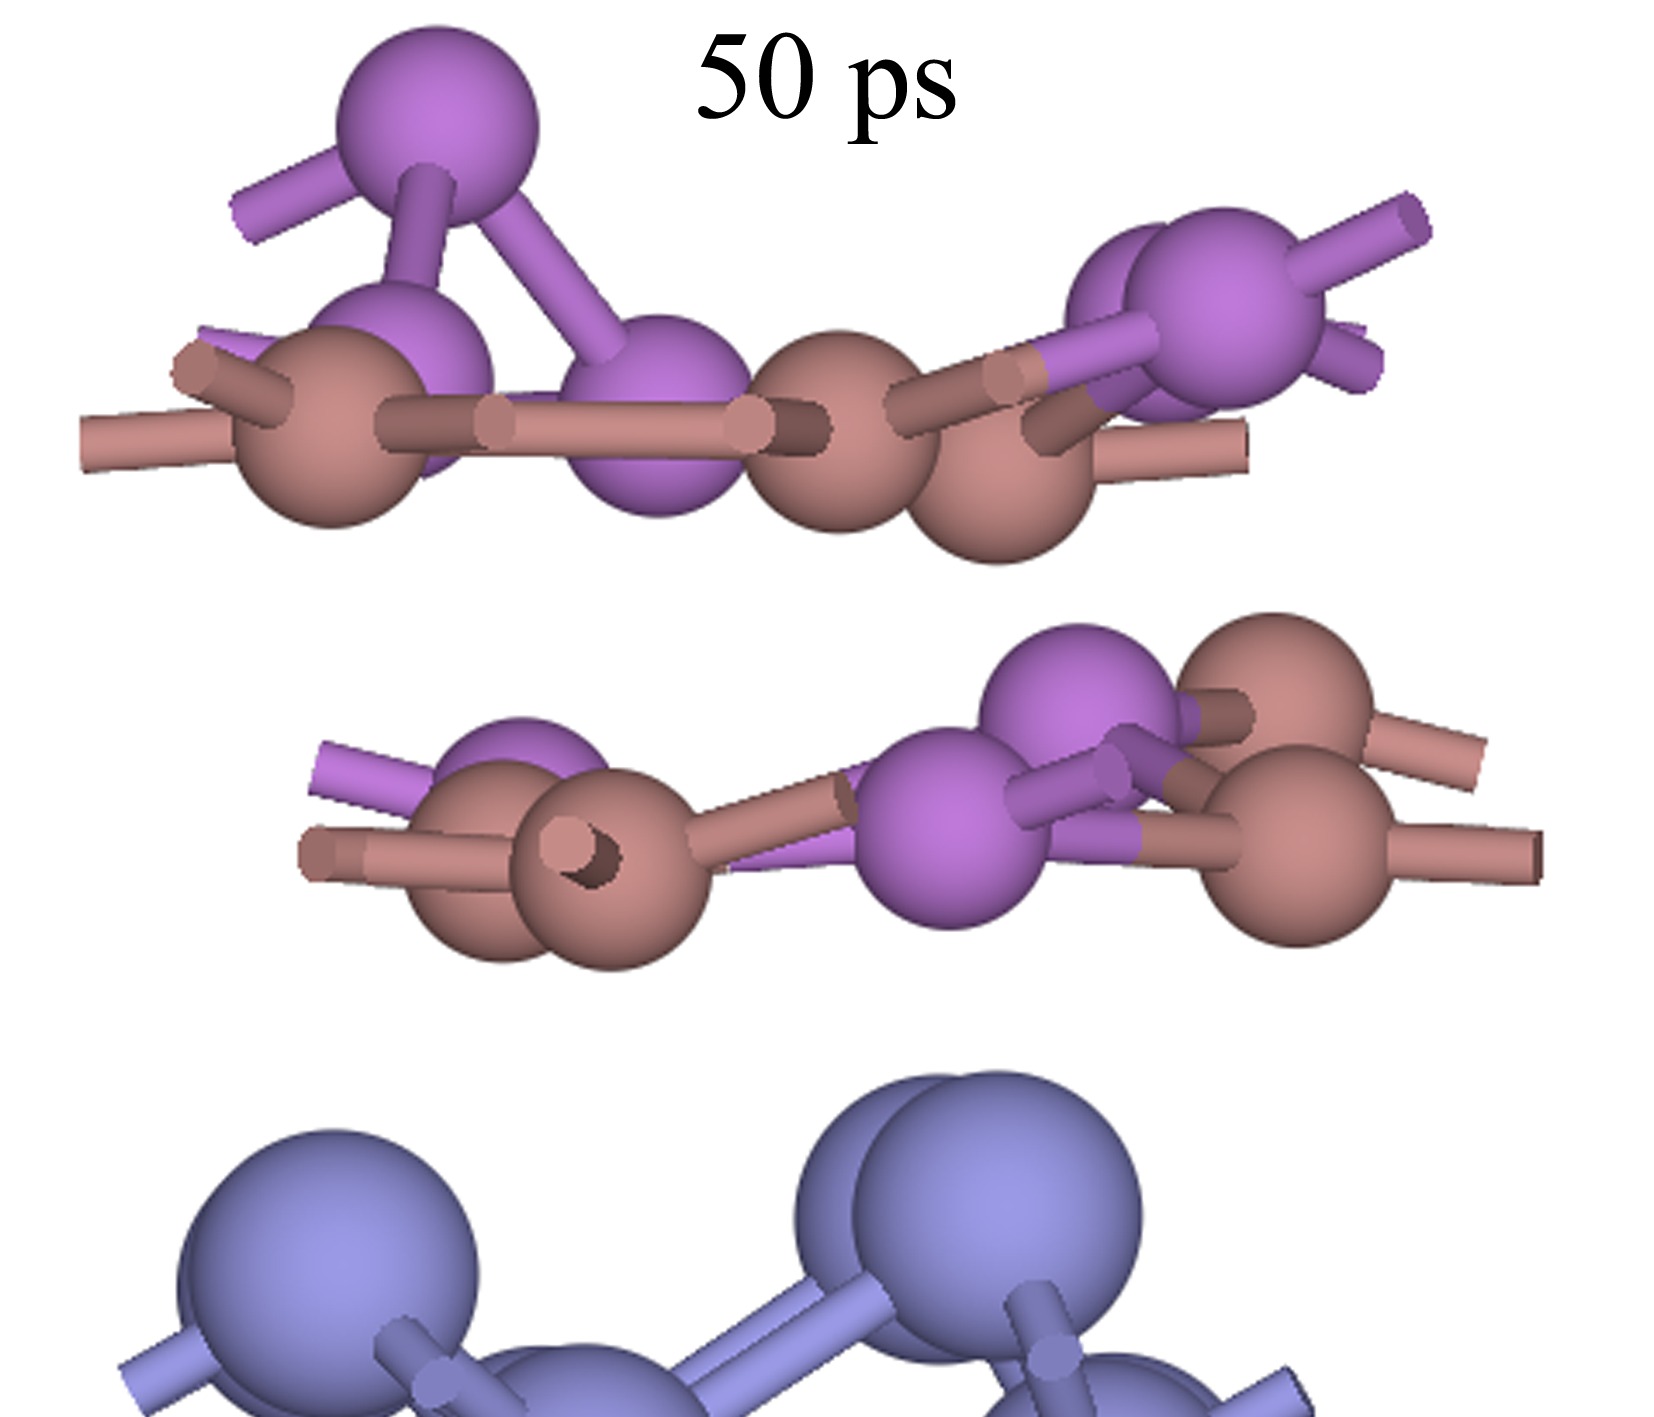
\includegraphics[width=0.4\textwidth]{pic/IS_structure_2Linsb_md50ps.png}
        \label{fig:IS_structure_2Linsb_md50ps}
    }
    \subfloat[]{
        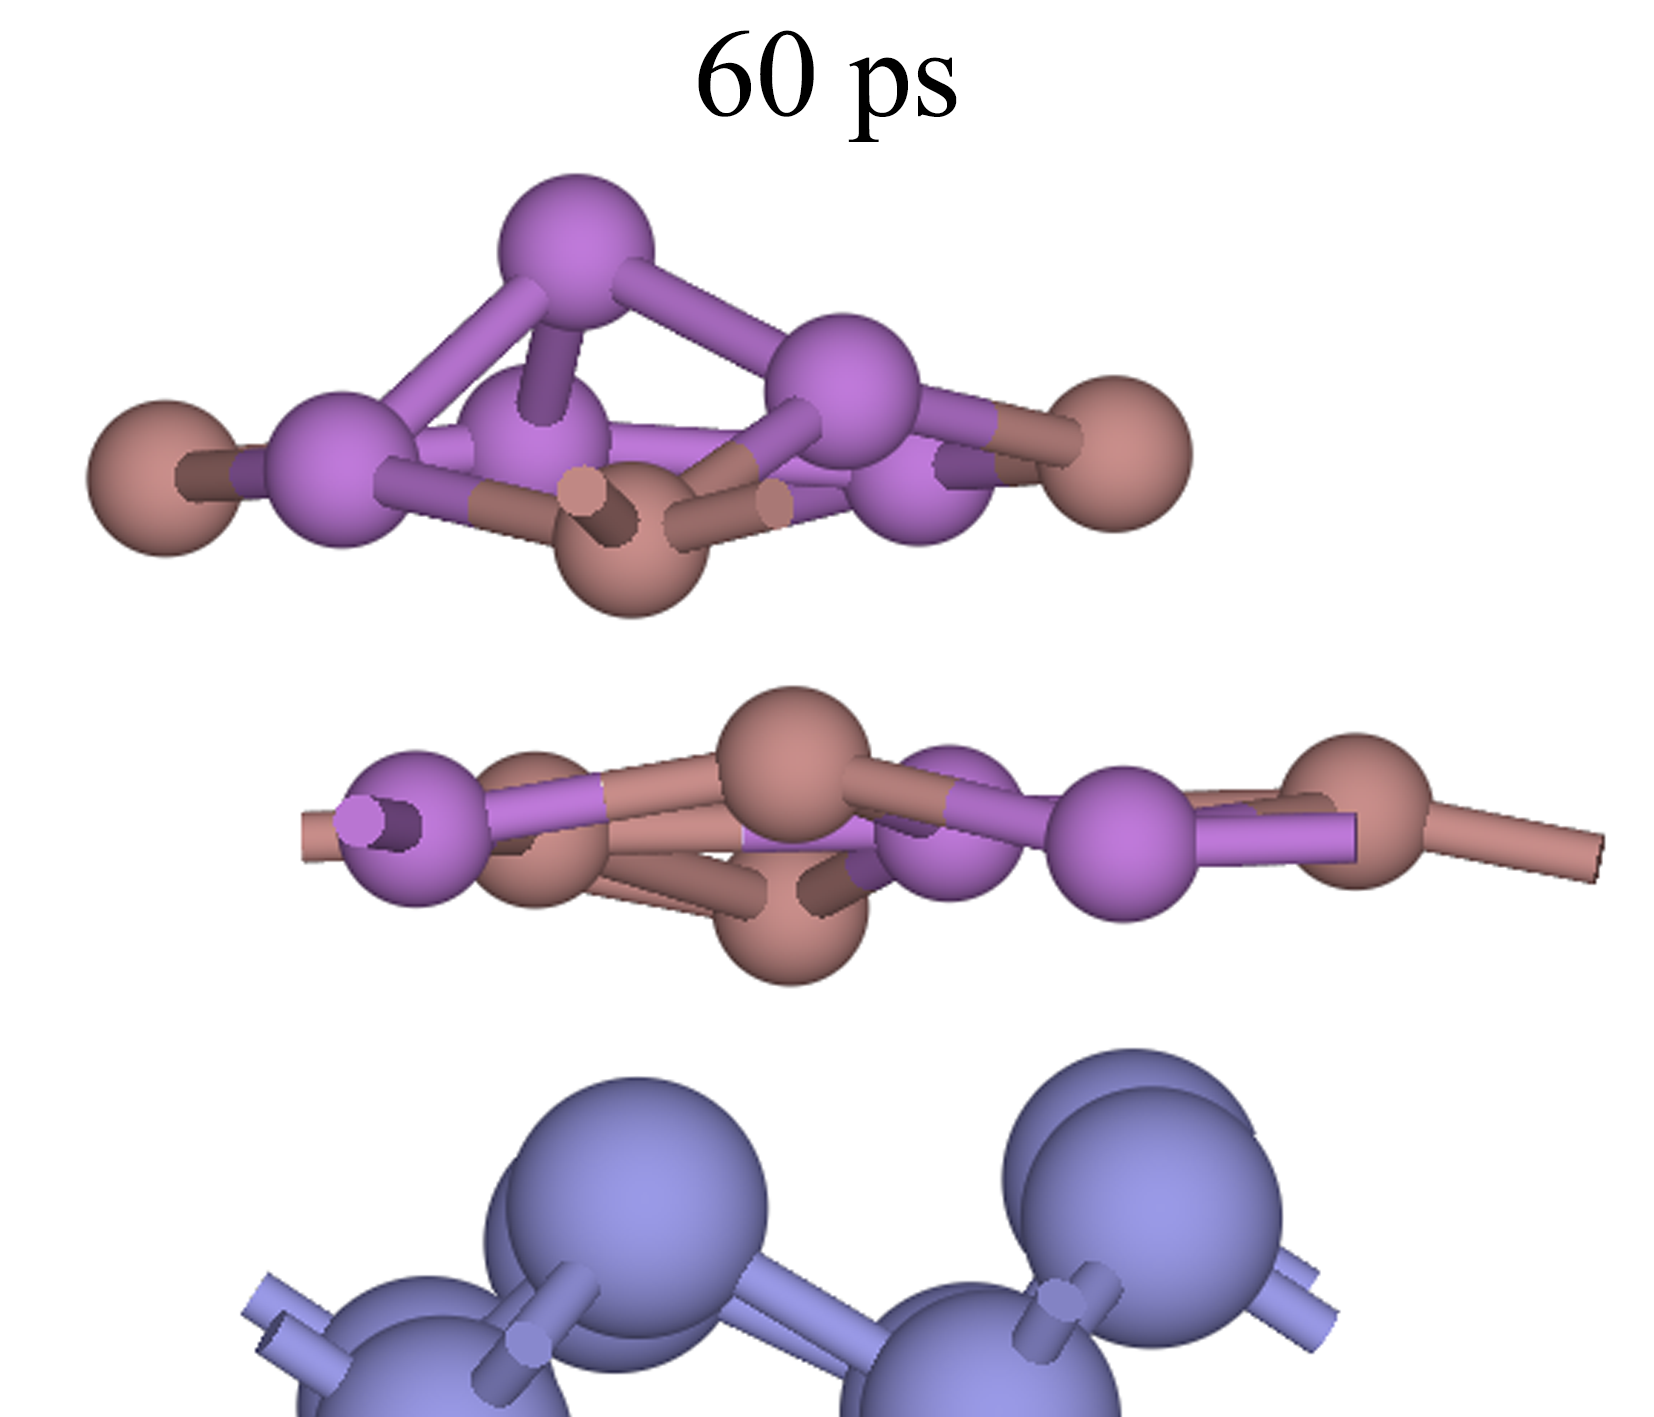
\includegraphics[width=0.4\textwidth]{pic/IS_structure_2Linsb_md60ps.png}
        \label{fig:IS_structure_2Linsb_md60ps}
    }\\[-0.5ex]
    \subfloat[]{
        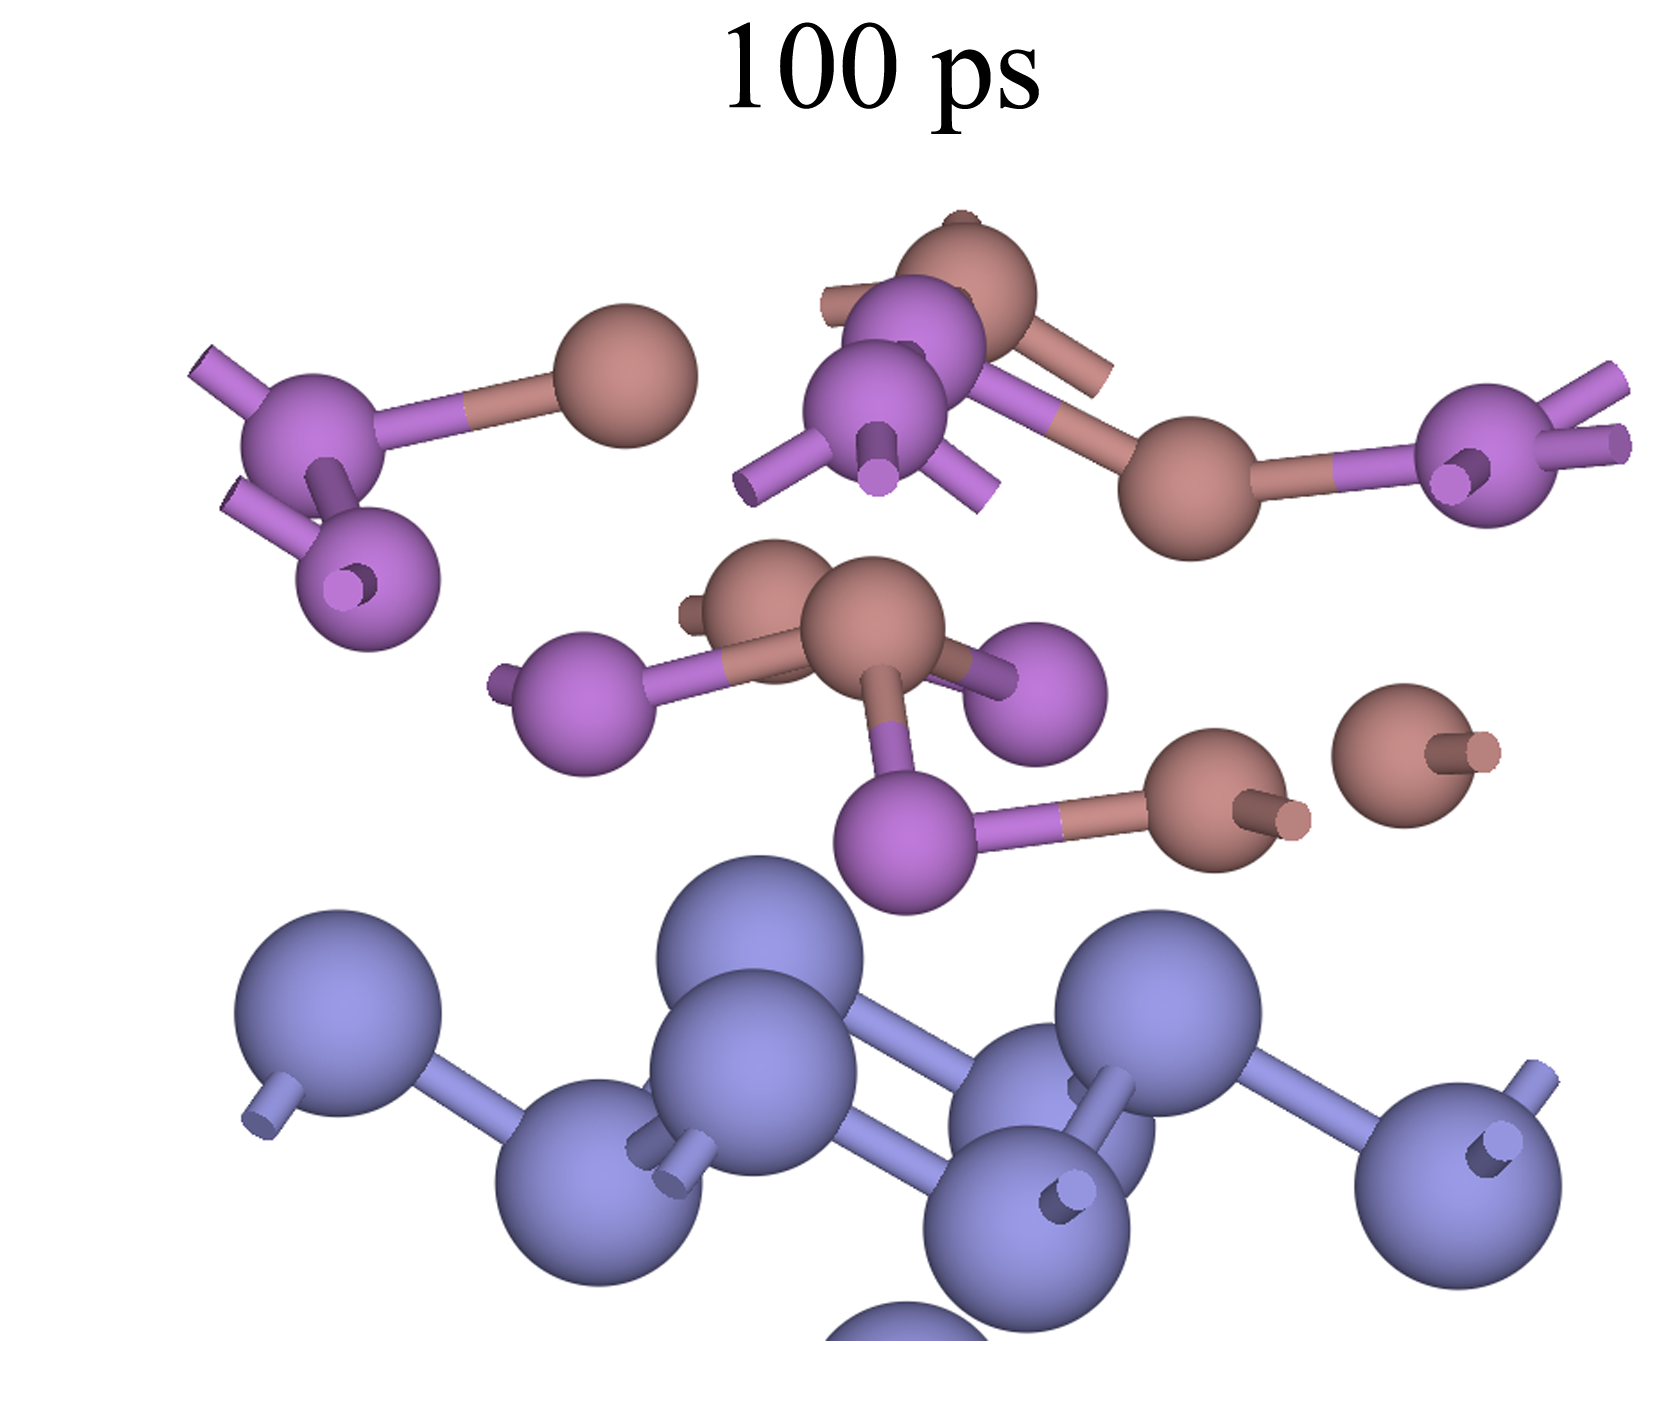
\includegraphics[width=0.4\textwidth]{pic/IS_structure_2Linsb_md100ps.png}
        \label{fig:IS_structure_2Linsb_md100ps}
    }
    \subfloat[]{
        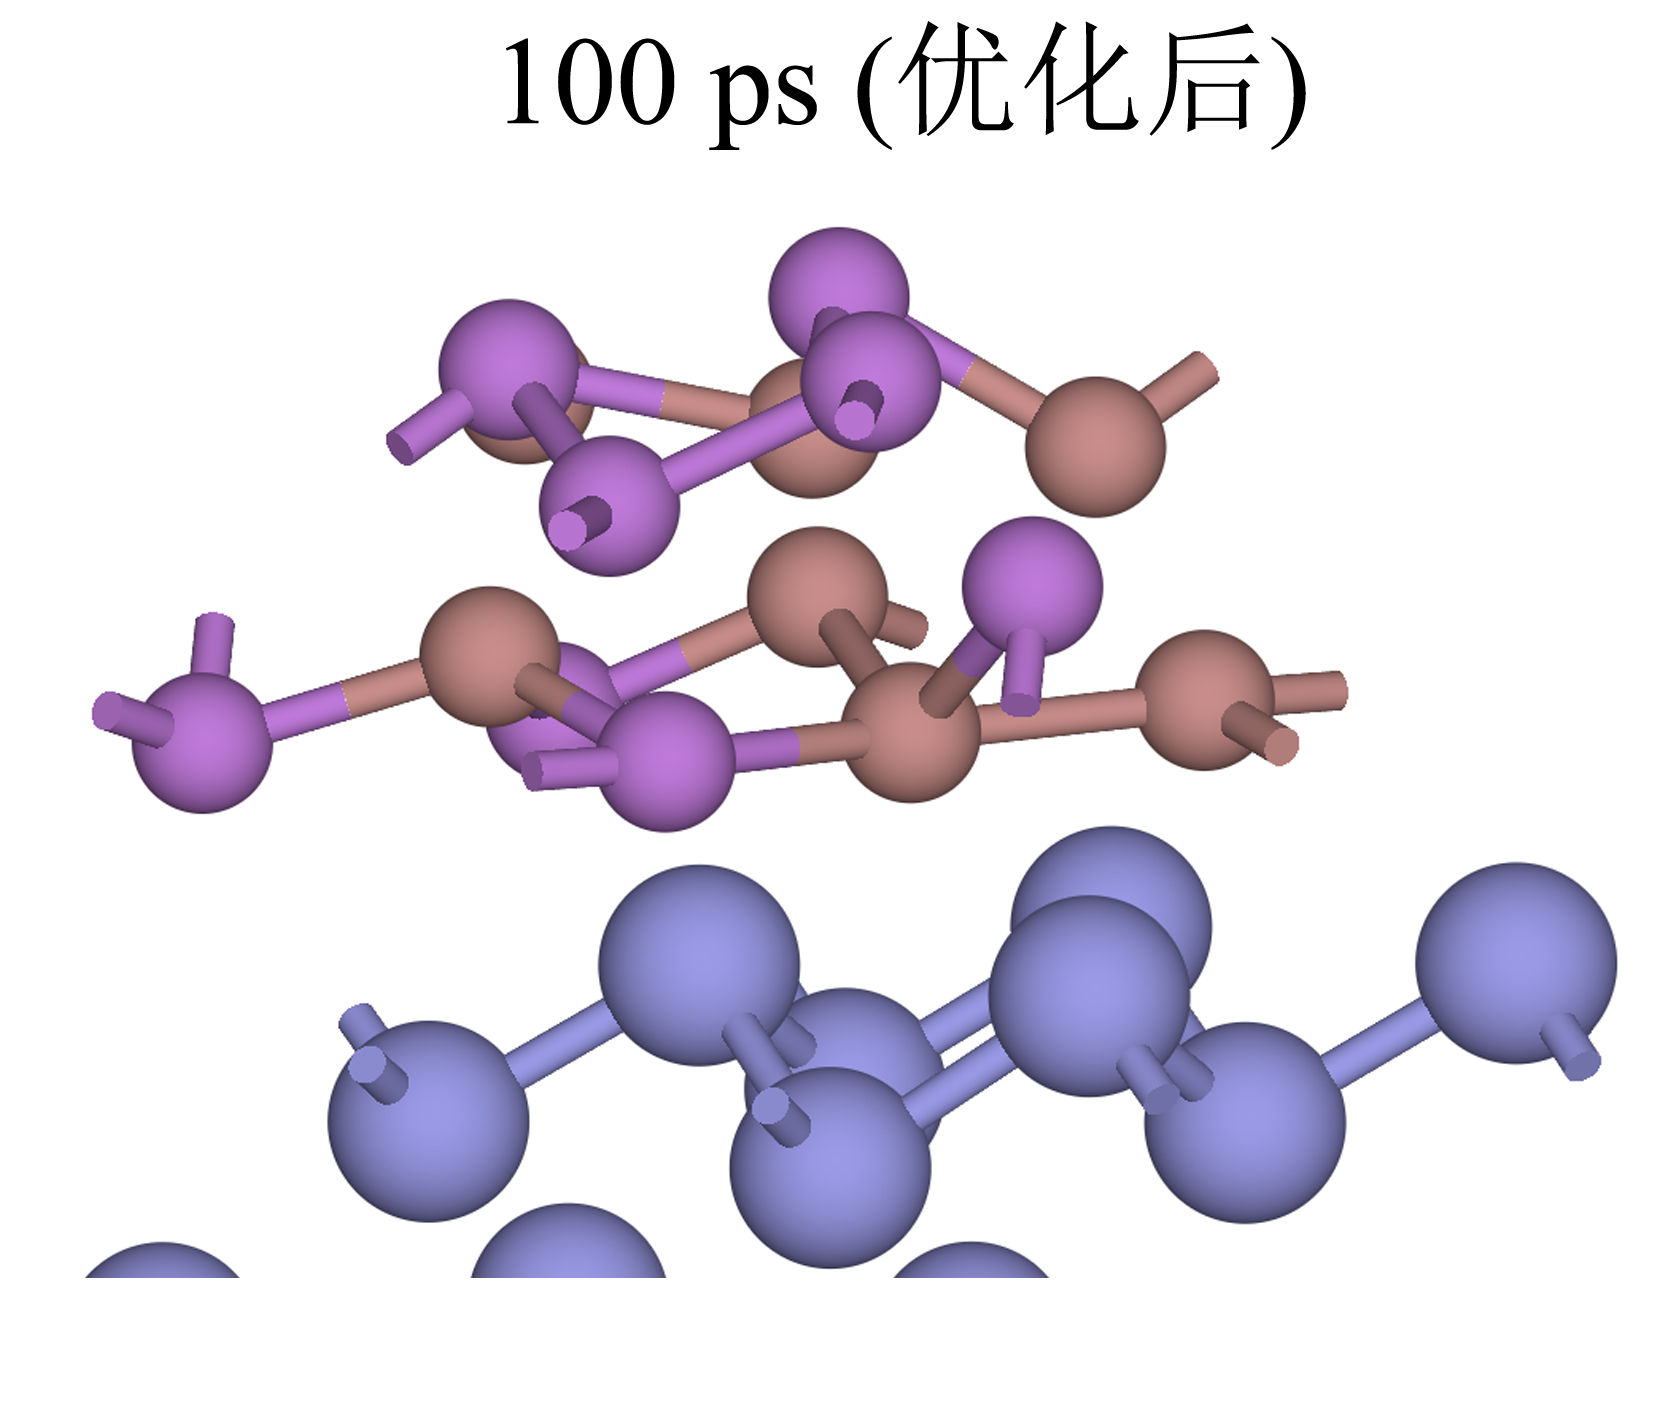
\includegraphics[width=0.4\textwidth]{pic/IS_structure_2Linsb_md100psopt.png}
        \label{fig:IS_structure_2Linsb_md100psopt}
    }
    \caption{\cemb{Bi(001)}衬底上双层\cemb{InSb}极性演化的分子动力学模拟结果。(a)分子动力学模拟50ps后的原子结构图;(b)分b动力学模拟60ps后的原子结构图;(c)分子动力学模拟100ps后的原子结构图;(d)100ps对应中间态的原子结构图。原子结构图中,\cemb{Bi}原子使用蓝色表示,\cemb{In}原子使用褐色表示,\cemb{Sb}原子使用紫色表示。}
    \label{fig:IS_structure_2Linsb_md}
\end{figure}

由于计算能力和模拟时长的限制,我们未能在模拟的时限内发现\cemb{In}空位重构层下第一层\cemb{InSb}完全转变为\cemb{In}极化构型。我们对进行了分子动力学模拟\SI{100}{\pico\second}后的双层\cemb{InSb}模型进行了结构优化,以去除分子动力学模拟中的热扰动热扰动,获得在热动能的驱动下,双层\cemb{InSb}极性演化的中间态。如图\ref{fig:IS_structure_2Linsb_md100psopt}所示,在经过结构优化后,双层\cemb{InSb}极性演化的中间态具有两个\cemb{In}次表面四面体,显示出半\cemb{In}极化的结构。同时,形成能的计算显示这个双层\cemb{InSb}极性演化的中间态的形成能介于\cemb{In}极性的第一层和$\InSbMLpolar{2}{2}$的第一层之间。进一步印证了在热动能的驱使下,双层\cemb{InSb}会逐渐从原本以混合极性为主的非晶态慢慢极化至\cemb{In}极性。

\begin{figure}[!htb]
    \subfloat[]{
        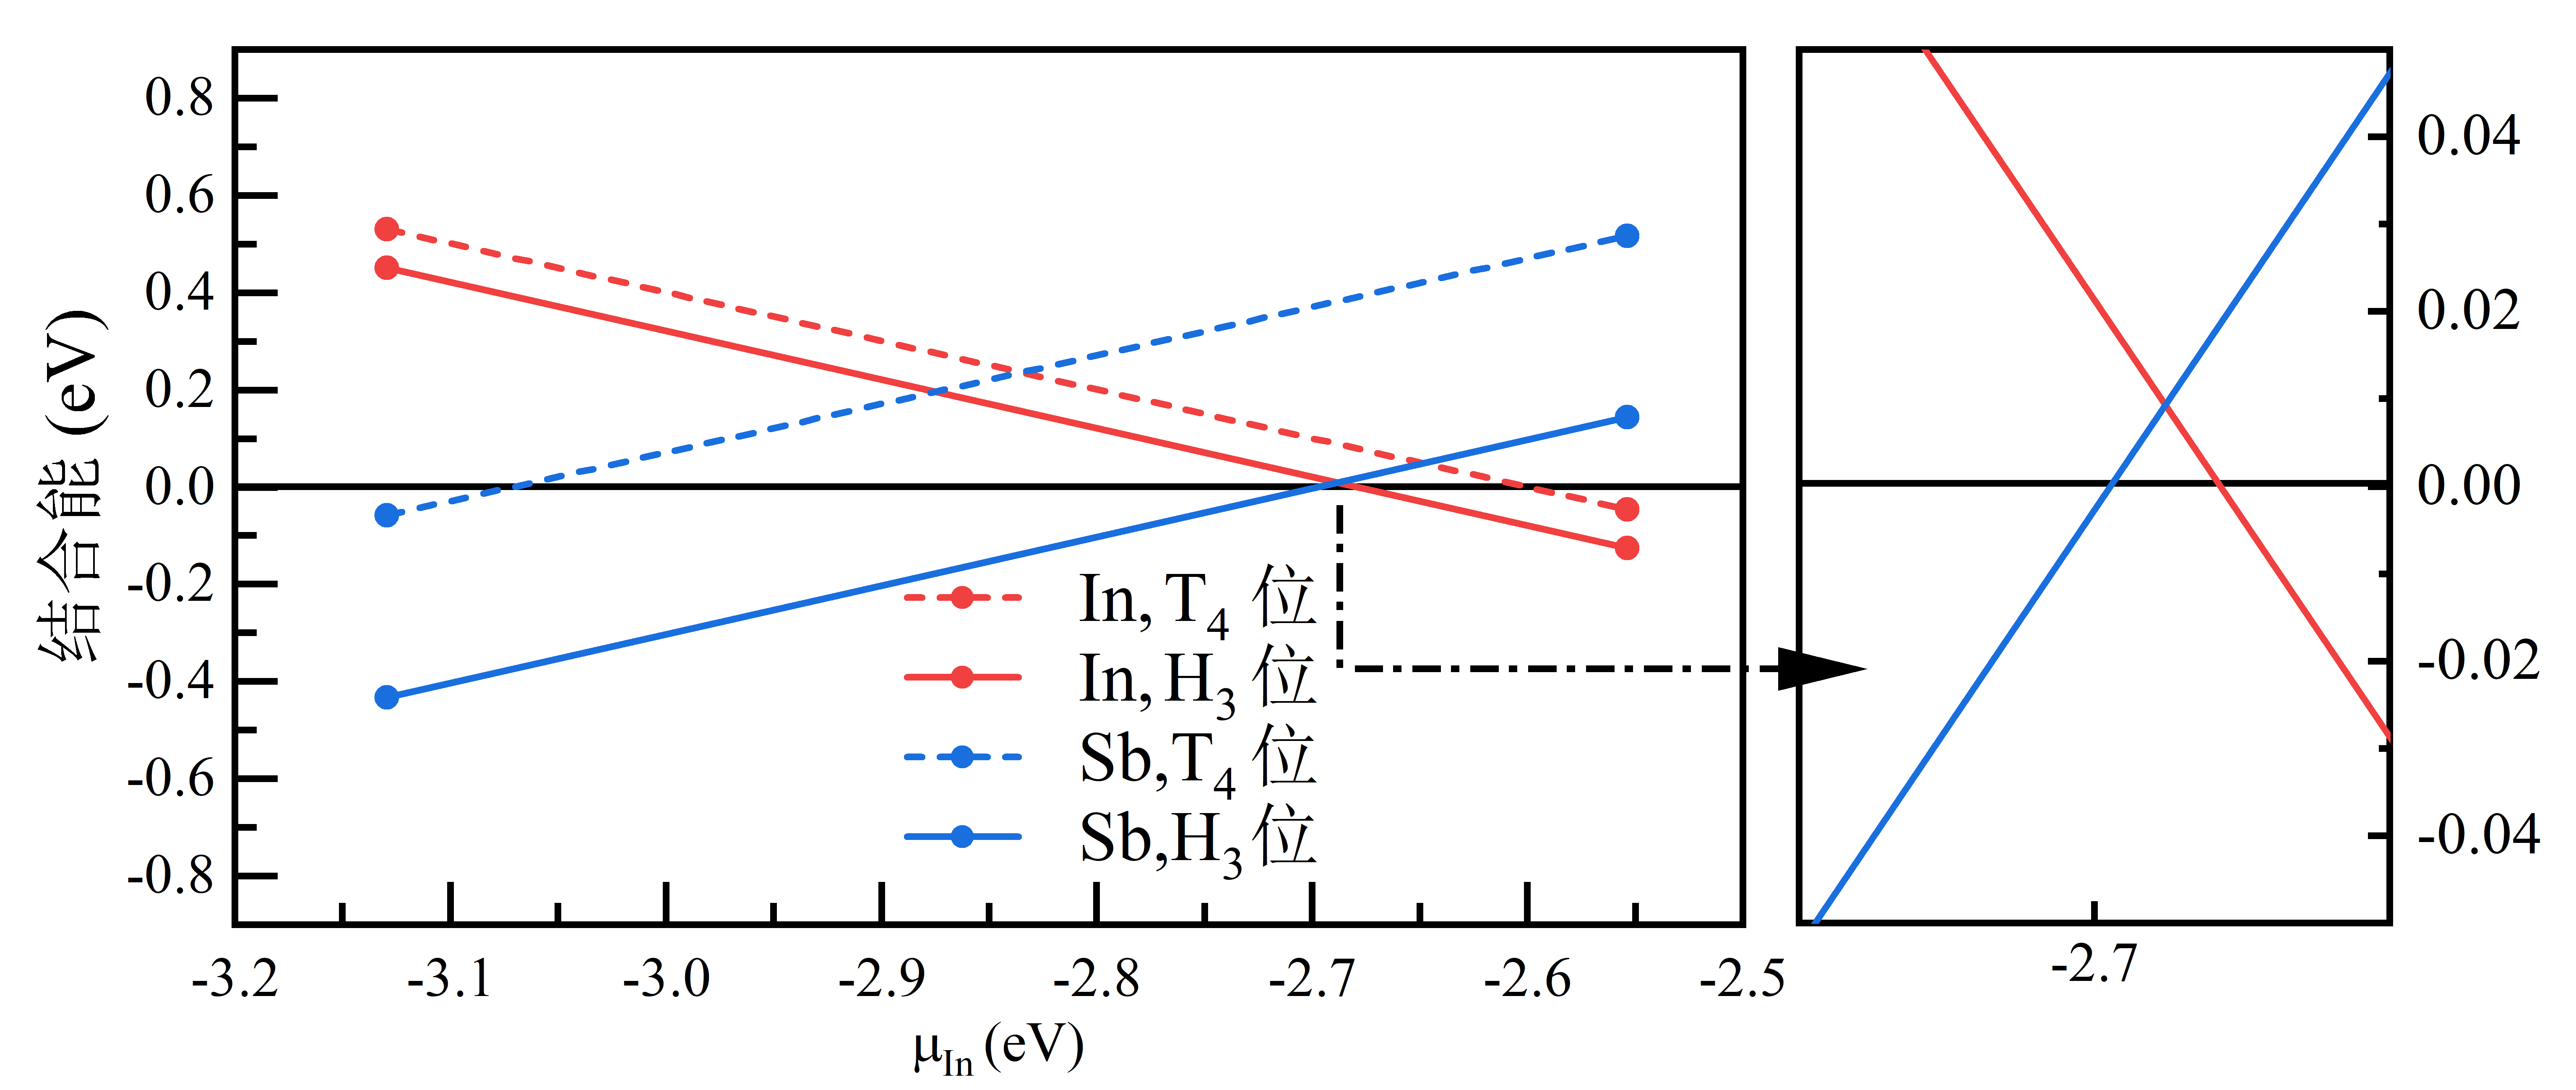
\includegraphics{pic/IS_DFT_2InSb_adatoms.png}
    }\\[-0.5ex]
    \subfloat[]{
        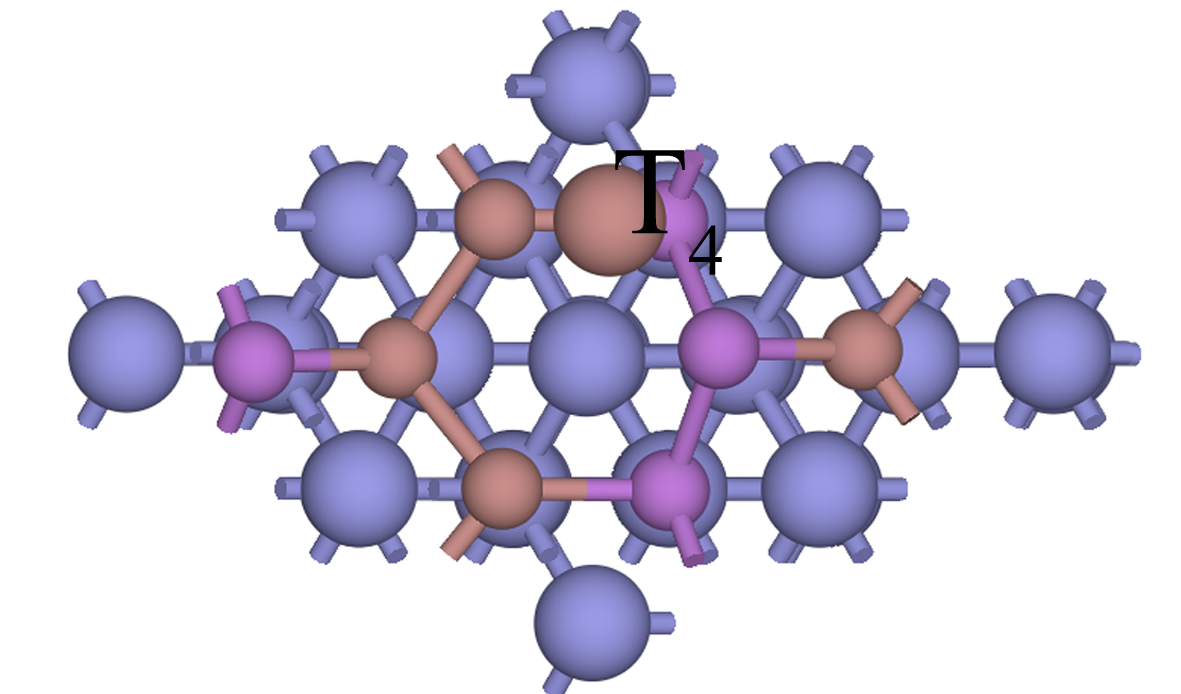
\includegraphics{pic/IS_structure_2Linsb_adatoms_InT4.png}
    }
    \subfloat[]{
        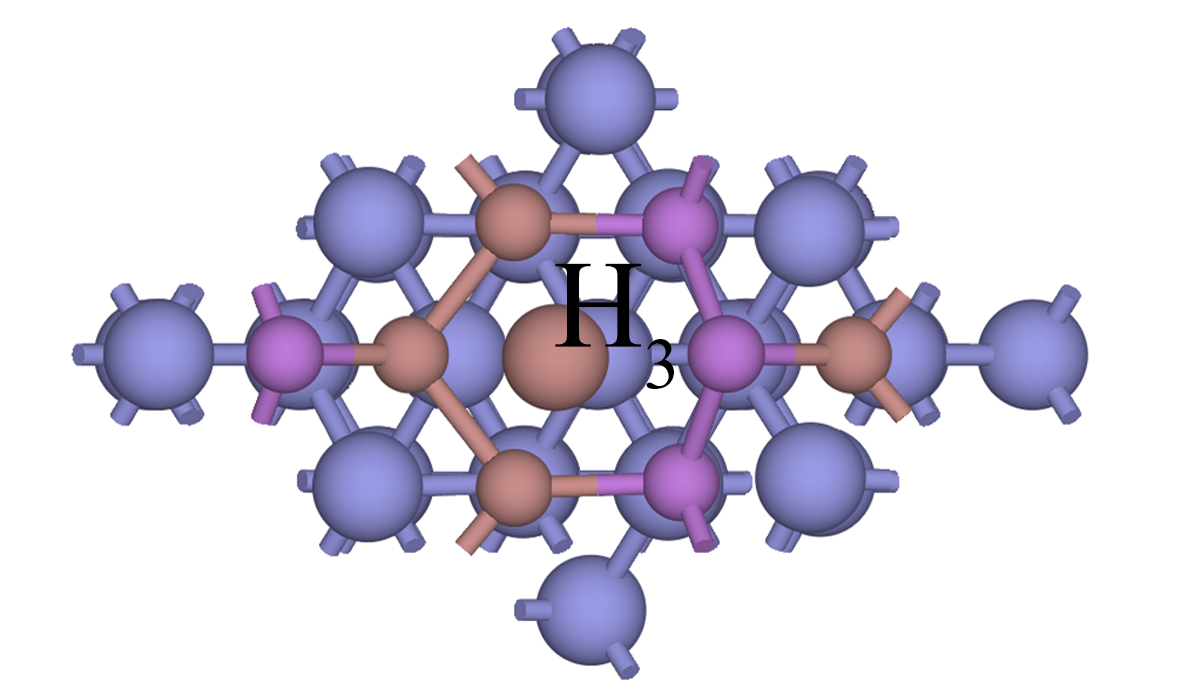
\includegraphics{pic/IS_structure_2Linsb_adatoms_InH3.png}
    }\\[-0.5ex]
    \subfloat[]{
        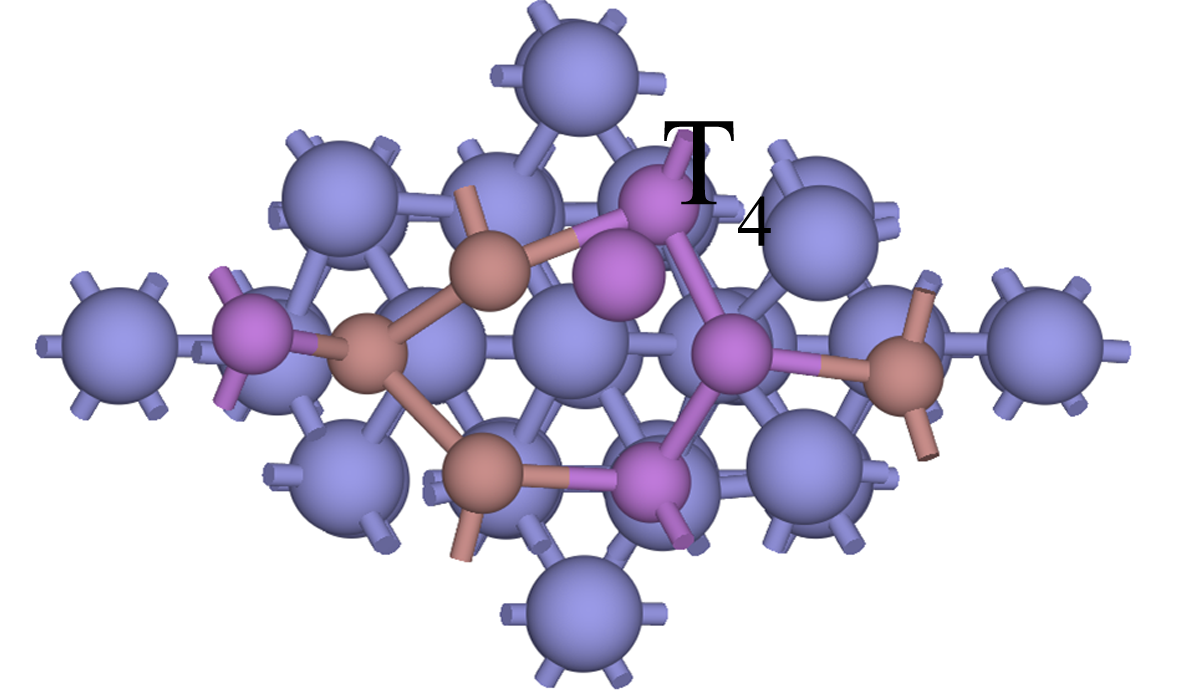
\includegraphics{pic/IS_structure_2Linsb_adatoms_SbT4.png}
    }
    \subfloat[]{
        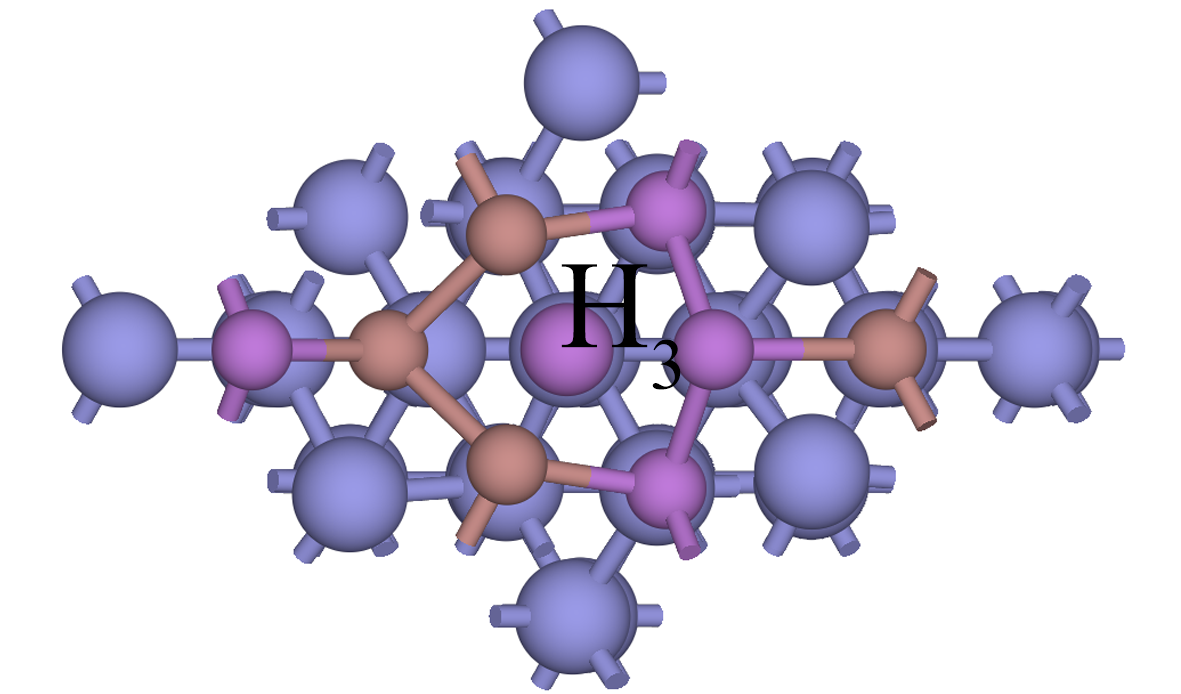
\includegraphics{pic/IS_structure_2Linsb_adatoms_SbH3.png}
    }
    \caption{\cemb{In}原子和\cemb{Sb}原子在\InSbMLpolar{2}{2}条形单层\cemb{InSb}表面吸附的结合能和吸附原子结构图。(a)吸附原子结合能;(b)\cemb{In}原子吸附在$\TfourSite$位;(c)\cemb{Sb}原子吸附在$\HthreeSite$位;(d)\cemb{In}原子吸附在$\TfourSite$位;(e)\cemb{Sb}原子吸附在$\HthreeSite$位。原子结构图中,\cemb{Bi}原子使用蓝色表示,\cemb{In}原子使用褐色表示,\cemb{Sb}原子使用紫色表示。}
    \label{fig:IS_2Linsb_adatom}
\end{figure}


为了揭示双层\cemb{InSb}的极化过程,我们首先对第二层\cemb{InSb}的生长过程进行探究。与在\cemb{Bi(001)}表面生长单层\cemb{InSb}类似,我们计算了\cemb{In}和\cemb{Sb}原子在单层\cemb{InSb}表面的吸附过程。考虑单层\cemb{InSb}以混合极性为主的非静态构型以及不同极性的形成能高低(图\ref{fig:IS_DFT_1LInSb_all}),我们选用$\InSbMLpolar{2}{2}$条形结构的单层\cemb{InSb}作为吸附表面。如图\ref{fig:IS_2Linsb_adatom}所示,我们同样考虑单层\cemb{InSb}表面$\TfourSite$位点和$\HthreeSite$位点对于\cemb{In}和\cemb{Sb}原子的吸附能力。与在\cemb{Bi}表面吸附不同,单层\cemb{InSb}对于\cemb{In}原子的吸附能力弱于\cemb{Sb}原子。在各自的浓度比例极限中,\cemb{Sb}原子吸附在\cemb{InSb}表面具有比\cemb{In}原子更高的结合能。同时,\cemb{Sb}原子与单层\cemb{InSb}更强的相互作用使得\cemb{Sb}原子吸附的为放热反应的$\muVar{In}{}$范围宽于\cemb{In}原子。对于\cemb{Sb}原子而言,其可以在生长环境中\cemb{In}原子浓度略高的情况下在单层\cemb{InSb}的表面吸附($\muVar{In}{}\leqslant \SI{-2.70}{\electronvolt}$)。而\cemb{In}原子只能在$\muVar{In}{} \geqslant \SI{-2.68}{\electronvolt}$的生长环境下才倾向于在单层的\cemb{InSb}表面吸附。在$\InSbMLpolar{2}{2}$条形结构的\cemb{InSb}的表面,没有能够同时吸附\cemb{In}原子和\cemb{Sb}原子的$\muVar{In}{}$窗口。因此,在第二层\cemb{InSb}成核生长的早期,由于生长环境中原子比例和化学活性的不同,在\cemb{In}和\cemb{Sb}之间只有一种原子能够直接在单层\cemb{InSb}表面吸附。我们可以通过调节生长环境中的浓度比例调控在单层\cemb{InSb}的优先吸附原子类型。

\begin{figure}[!htb]
    \subfloat[]{
        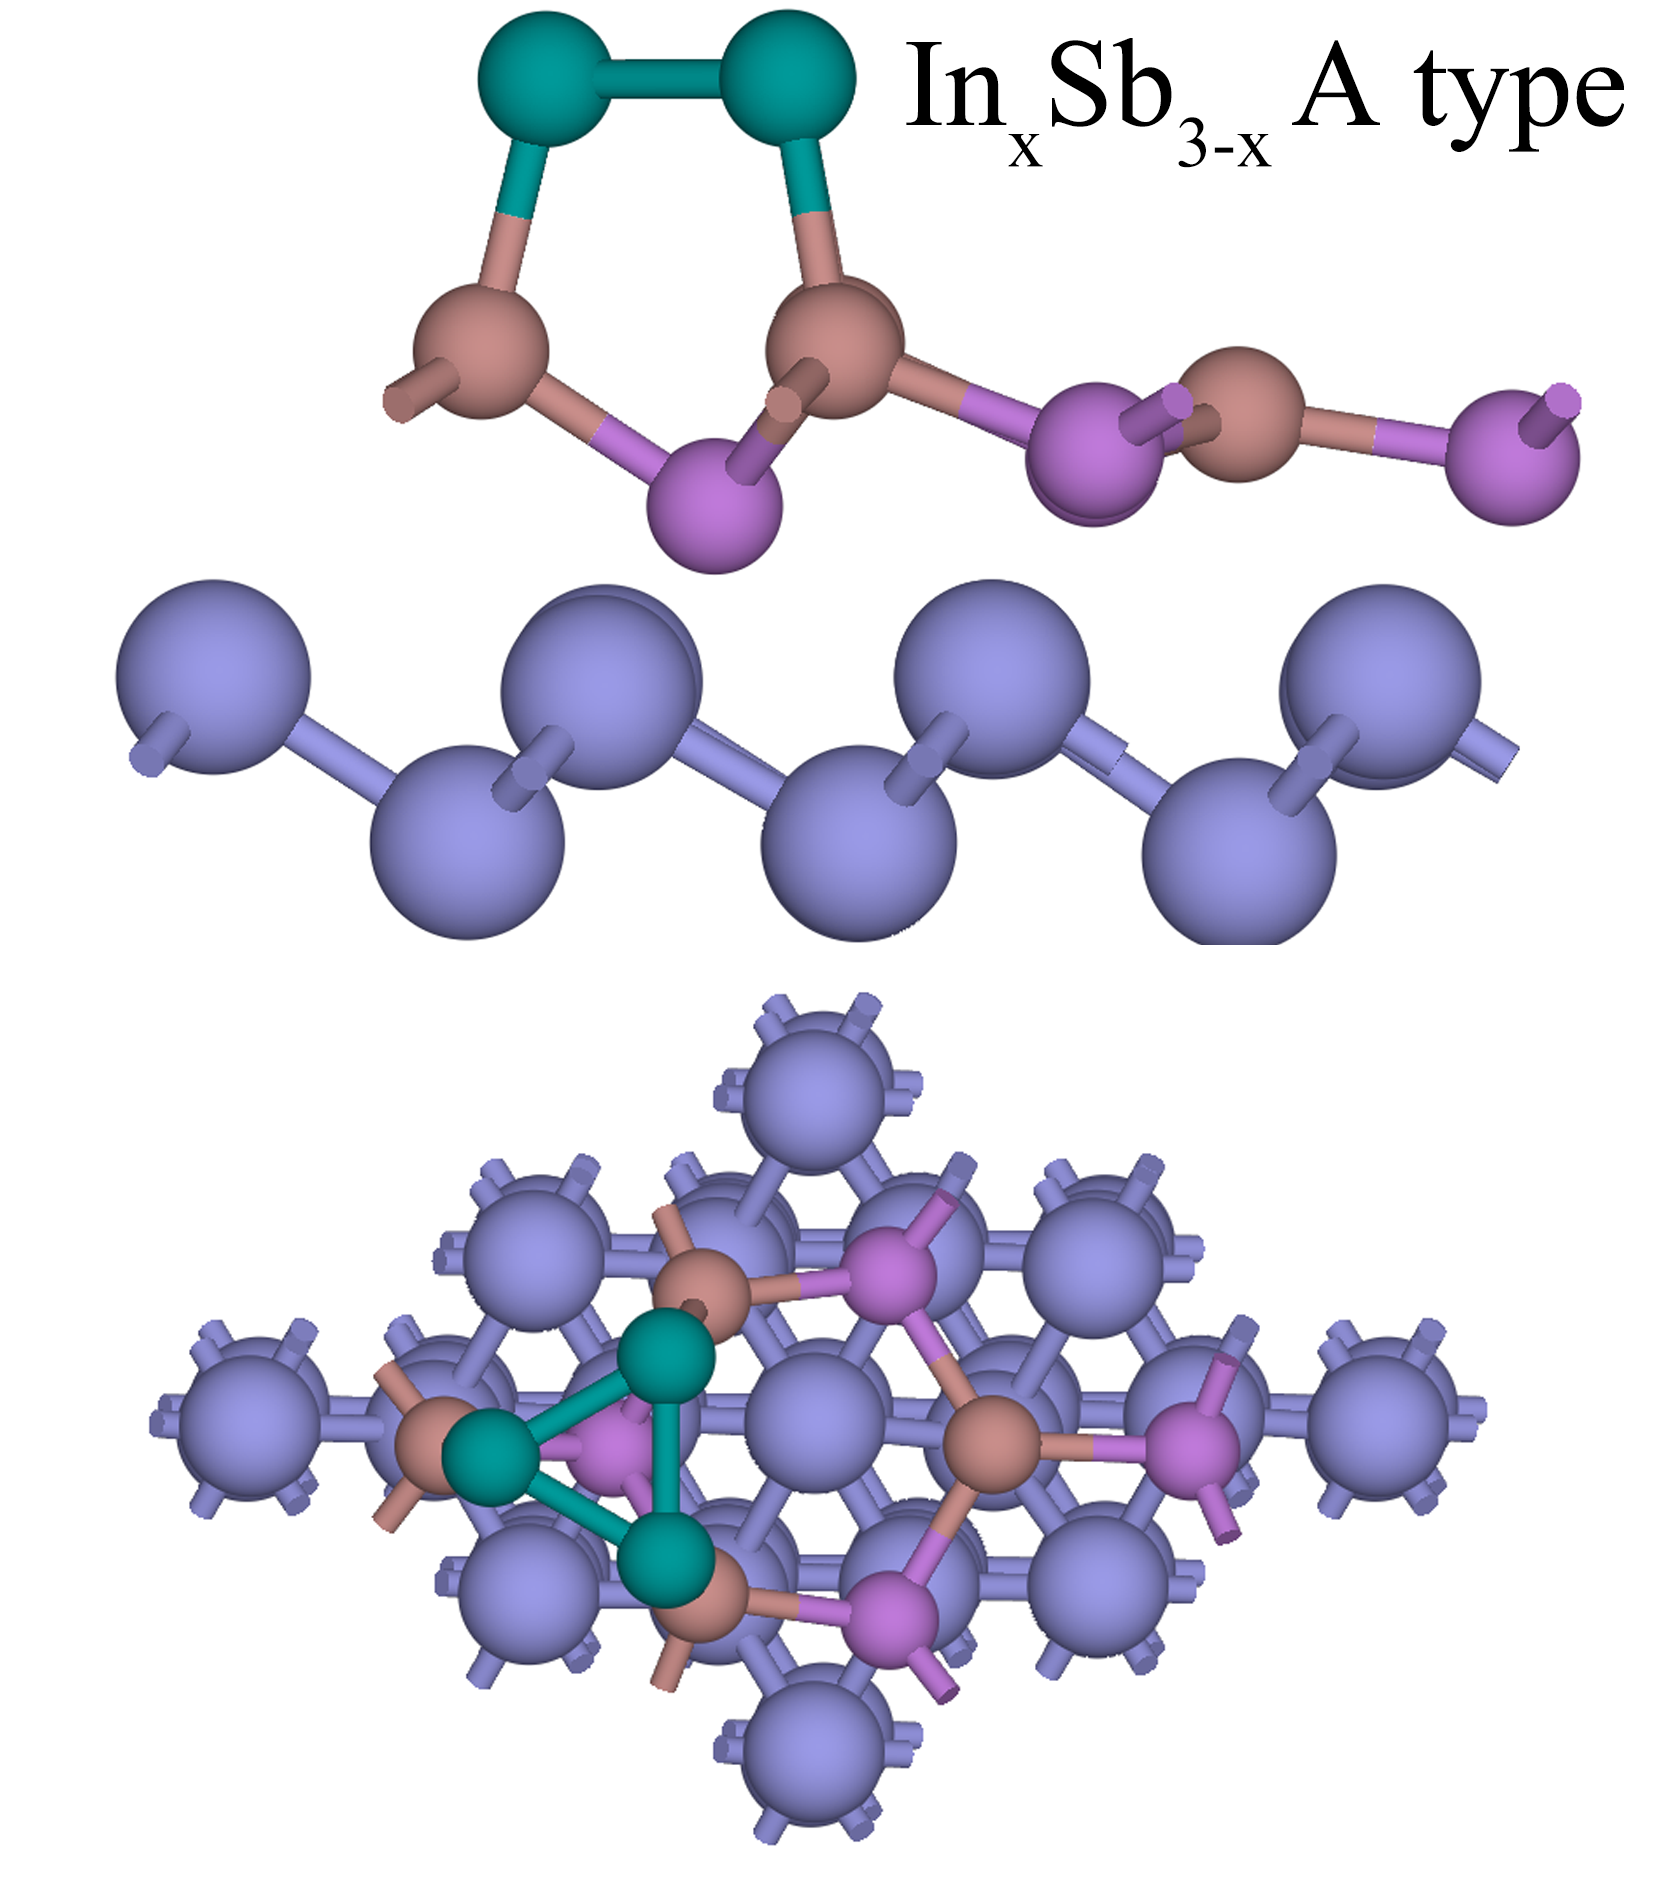
\includegraphics{pic/IS_structure_InxSb3-x_A.png}
    }
    \subfloat[]{
        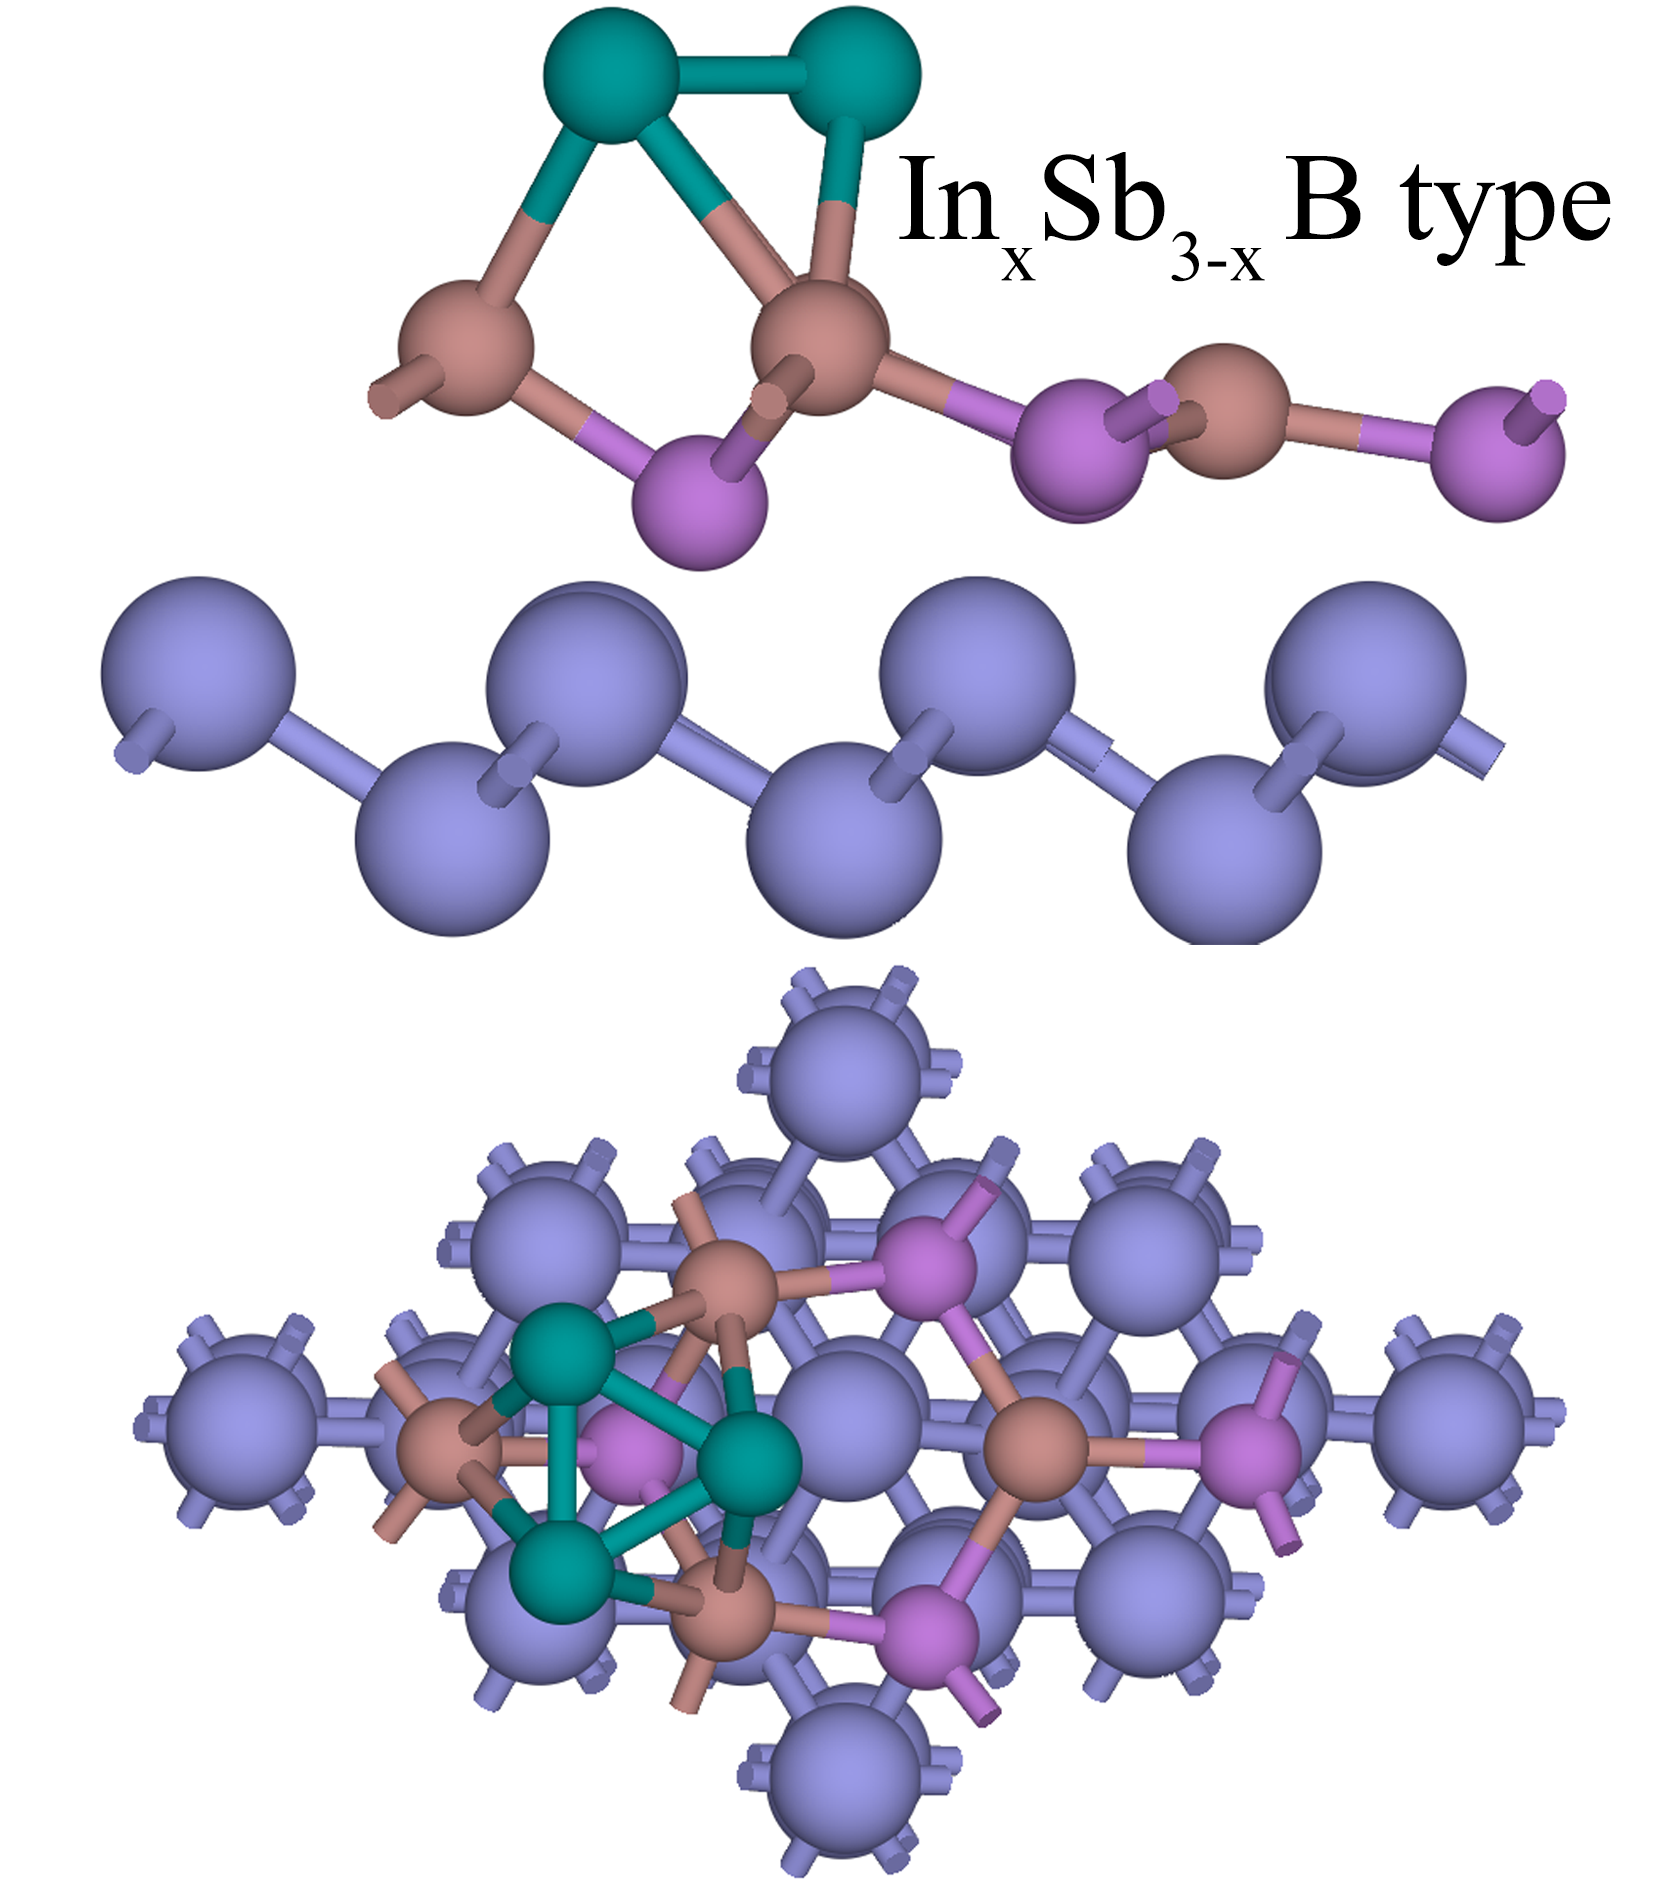
\includegraphics{pic/IS_structure_InxSb3-x_B.png}
    }
    \caption{单层\cemb{InSb}表面生长团簇(\cemb{In_xSb_{3-x}})的构型。(a)A类\cemb{In_xSb_{3-x}}团簇的原子构型;(b)B类\cemb{In_xSb_{3-x}}团簇的原子构型}
    \label{fig:IS_structure_InxSb3-x}
\end{figure} 

随着生长的进行,原本难以在单层\cemb{InSb}表面吸附的原子可能和已吸附的原子成键,形成团簇。团簇的生长形态和化学组成同样可能受到生长环境中$\muVar{In}{}$变化的影响。考虑第二层为到\cemb{Sb}三聚体重构时,于双层\cemb{InSb}的形成能谱(图\ref{fig:IS_DFT_2LInSb_SbTonAll})可以认为第一层混合极性的\cemb{InSb}的晶体化转变开始于作为第二层的\cemb{Sb}团簇重构层将第一层引导至理想极性的构型(\cemb{In}极性或者\cemb{Sb}极性)。同时,我们注意到从原子结构的角度看,\cemb{In}空位重构的原子结构可以由\cemb{Sb}三聚体重构表面继续吸附三个\cemb{In}原子和一个\cemb{Sb}原子形成。因此,在生长的过程中,\cemb{In}重构表面的第二层可能是从团簇阶段的\cemb{Sb}三聚体重构表面演化而来,并在\cemb{Sb}三聚体重构的第二层基础上进一步将第一层多晶态的\cemb{InSb}完全极化至\cemb{In}极性。

在生长过程的团簇阶段,我们需要验证\cemb{Sb}三聚体是否是生长过程中最为可能的团簇形态。因此,我们进一步考察了团簇生长阶段不同形貌的三聚体在\cemb{InSb}自极化过程中的形貌以及作为第二层的\cemb{InSb}团簇在不同$\muVar{In}{}$环境下的演化规律。通过先前的计算,我们已经得知作为第二层的\cemb{Sb}三聚体重构可以将原本极性混乱的第一层\cemb{InSb}引导至\cemb{In}极性或者\cemb{Sb}极性。而\cemb{In}极性的第一层构型是以\cemb{Sb}三聚体重构为第二层的双层石墨烯的的全局能量最低态。因此,我们将第一层构型的关注点限定在\cemb{In}极性,考察不同元素比例的\cemb{In_xSb_{3-x}}三聚体的生长机理。我们将\cemb{In}极性\cemb{InSb}上生长的\cemb{In_xSb_{3-x}}三聚体分为两类(图\ref{fig:IS_structure_InxSb3-x}),A类的构型和先前所计算的\cemb{Sb}三聚体类似,三聚体内部的原子处于$\TfourSite$位三角形的顶点位。B类构型由A类构型在平面内旋转\SI{60}{\degree}得到,其三聚体内部的原子处于$\TfourSite$位三角形的边位。

\begin{figure}[!htb]
    \subfloat[]{
        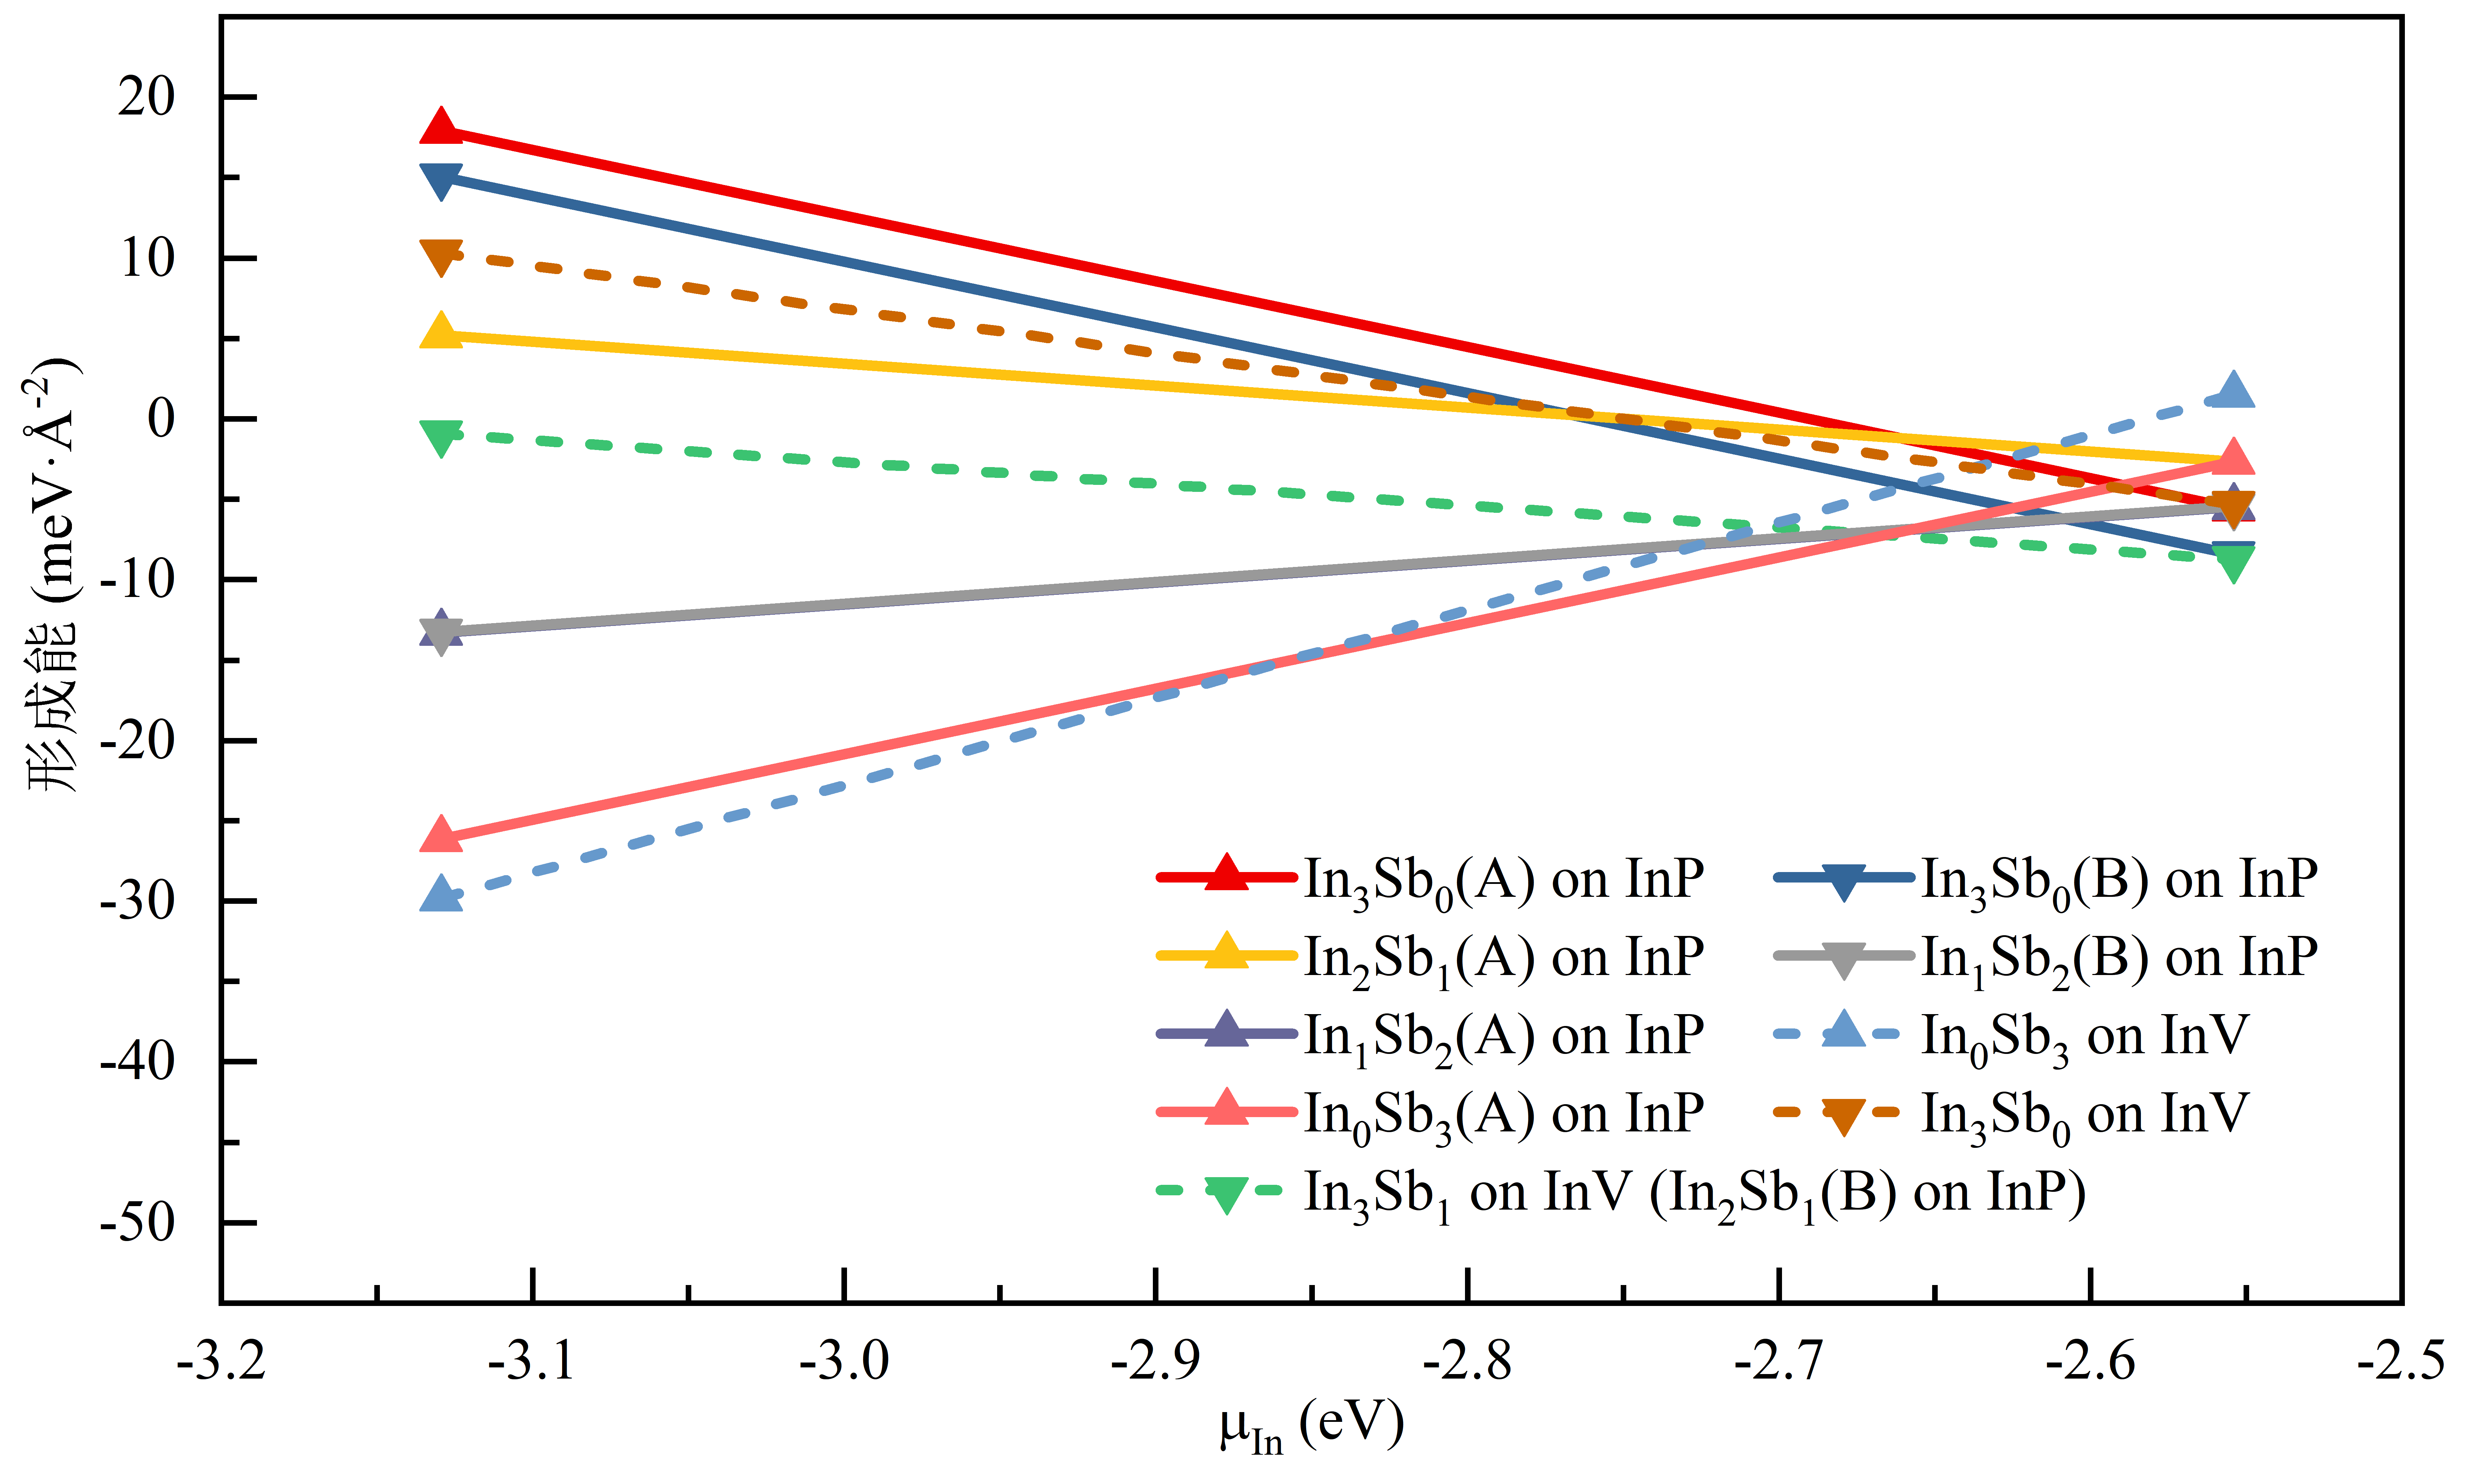
\includegraphics[width=0.9\textwidth]{pic/IS_DFT_2InSb_InxSbxT_All.png}
    }\\[-1ex]
    \subfloat[]{
        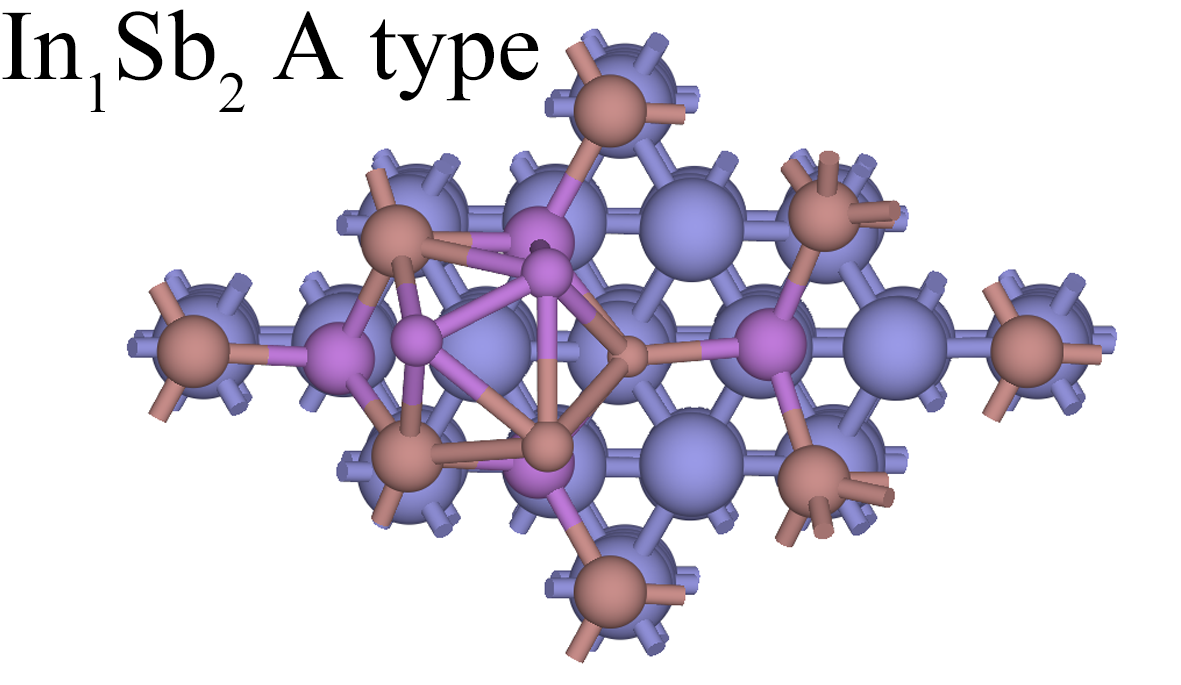
\includegraphics{pic/IS_structure_In1Sb2_A.png}
    }
    \subfloat[]{
        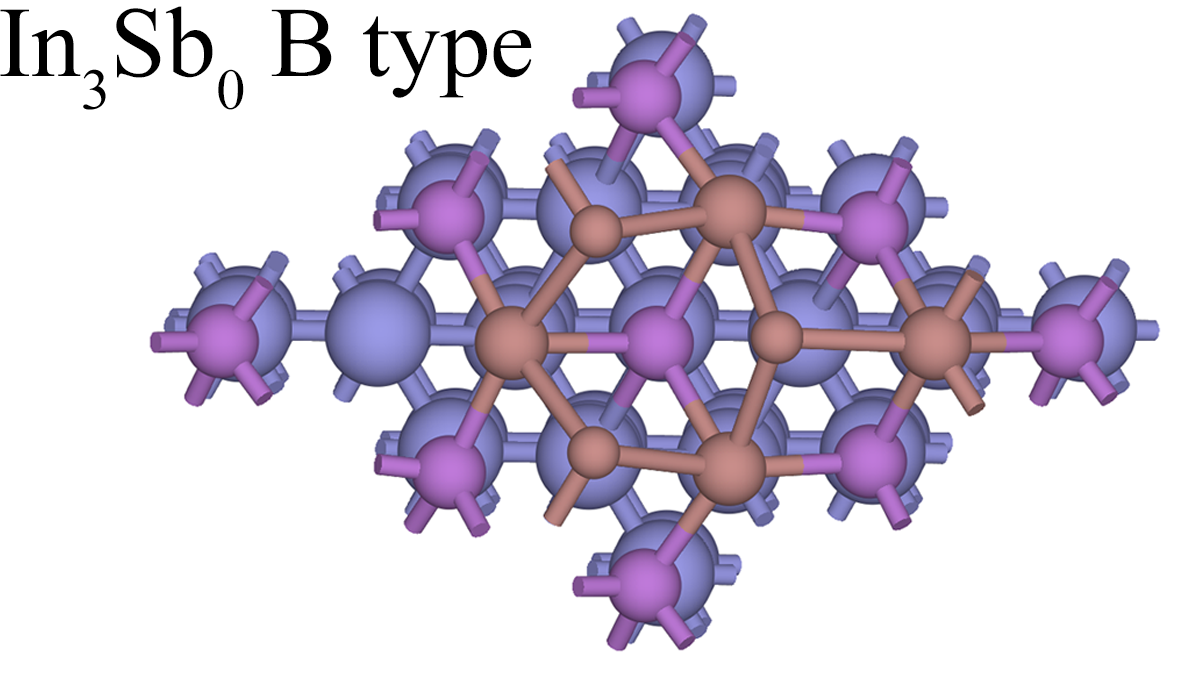
\includegraphics{pic/IS_structure_In3Sb0_B.png}
    }
    \caption{单层\cemb{InSb}表面\cemb{In_xSb_{3-x}}团簇的形成能及代表性团簇结构原子构型。(a)不同化学计量比\cemb{In_xSb_{3-x}}团簇的形成能分布;(b)A类\cemb{In1Sb2}的原子构型;(c)B类\cemb{In3Sb0}的原子构型。}
    \label{fig:IS_DFT_2InSb_InxSbxT_All}
\end{figure}

在图\ref{fig:IS_DFT_2InSb_InxSbxT_All}中,我们计算了在\cemb{In}极性的\cemb{InSb}表面生长不同化学计量比的\cemb{In_xSb_{3-x}}团簇的形成能情况。整体来看,随着\cemb{Sb}原子化学计量比的上升,\cemb{In_xSb_{3-x}}团簇的形成能逐渐下降。在所有考虑的团簇中, A类\cemb{In0Sb3}团簇(\cemb{Sb}三聚体重构)的形成能在在大部分的$\muVar{In}{}$条件下取到最低值。这与\cemb{Sb}三聚体重构作为生长实验中自然形成的\cemb{Sb}极性的表面重构现象一致\citing{RN896-1998}。而包含\cemb{In}元素的团簇仅在生长环境中\cemb{In}原子浓度较高,$\muVar{In}{}$的取值接近纯\cemb{In}极限时才有能量上的优势。

从原子结构的角度看,\cemb{Sb}原子在\cemb{InSb}表面形成的重构倾向于保持A类团簇的构型,而\cemb{In}原子组成的重构则倾向于形成B类团簇的结构。在\cemb{InSb}混合团簇的原子结构中,\cemb{In}的加入更倾向于单独吸附在$\TfourSite$位点,破坏了\cemb{Sb}三聚体在\cemb{InSb}表面的等边三角形构型。对于只含有\cemb{In}原子的\cemb{In3Sb0}团簇,结构优化的结果显示第二层的\cemb{In}原子之间仅存在非常弱的相互作用。这个较弱的相互作用只将原本各自独立吸附在$\TfourSite$位和$\HthreeSite$位的\cemb{In}原子向团簇的中心偏移了很小的位移。综合以上的计算结果,我们可以认为在生长第二层\cemb{InSb}以及双层\cemb{InSb}的自极化过程中,团簇阶段主要以\cemb{Sb}三聚体的形式存在。而在团簇阶段中\cemb{InSb}第一层表面的\cemb{In}原子则主要以较为分散的吸附原子的形式存在。

\begin{figure}[!htb]
    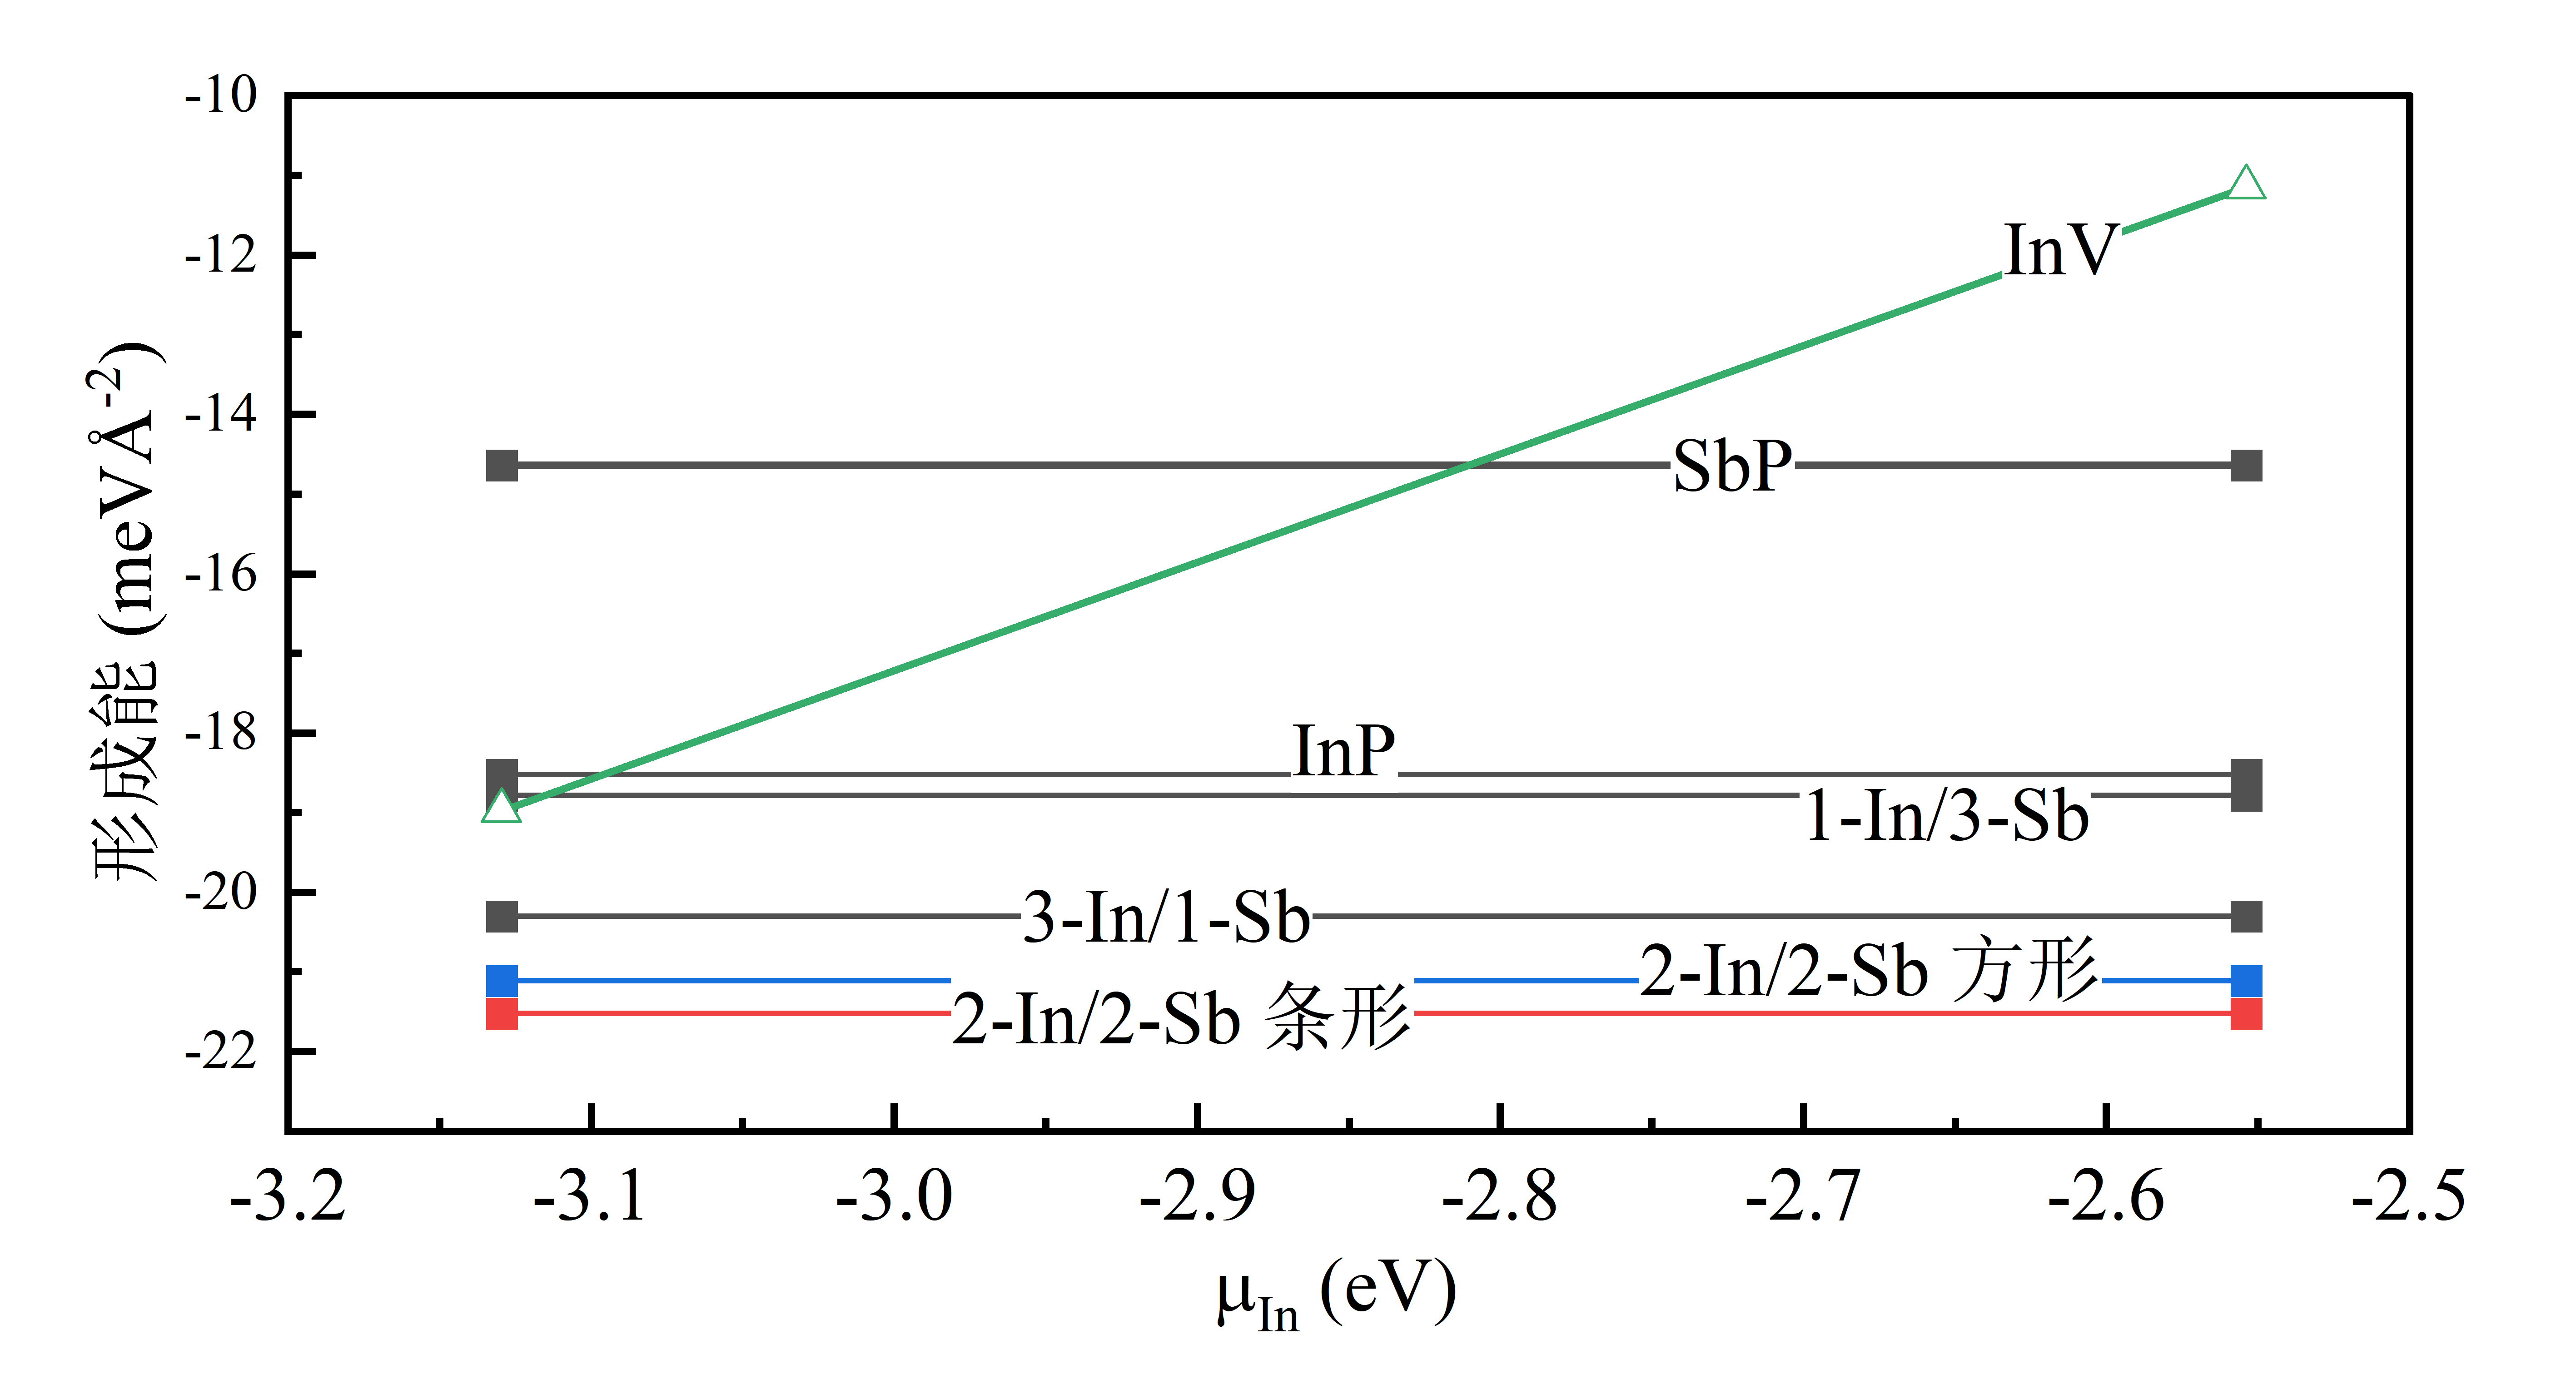
\includegraphics{pic/IS_DFT_1InSb_FlipVsInV.png}
    \caption{\cemb{Bi(001)}表面不同极性单层\cemb{InSb}和\cemb{In}空位重构层的形成能对比。}
    \label{fig:IS_DFT_1InSb_FlipVsInV}
\end{figure}

此外,我们发现在B形状\cemb{In2Sb1}第二层下方的\cemb{In}极性\cemb{InSb}在在原子优化后变为了\cemb{In}空位层。多余的\cemb{In}原子被挤入第二层的团簇之中,形成了
包含三个\cemb{In}原子的\cemb{In}三聚体。我们同时检查了\cemb{In}空位的重构构型在单层\cemb{InSb}中的形成能情况。如图\ref{fig:IS_DFT_1InSb_FlipVsInV}所示,只有在接近纯\cemb{Sb}环境的情况下,在\cemb{Bi(001)}表面\cemb{In}空位的形成能略低于\cemb{In}极性单层和\InSbMLpolar{1}{3}混合极性单层的形成能。随着生长环境中\cemb{In}原子浓度的上升,\cemb{In}原子的活性上升,环境中的\cemb{In}原子会倾向于填补\cemb{InSb}中的\cemb{In}空位,导致\cemb{In}空位的形成能也上升并且会超过\cemb{Sb}极性的单层\cemb{InSb}的形成能。

在\cemb{Sb}三聚体的和$\muVar{In}{}$的作用下,双层\cemb{InSb}中第一层的原子结构可以在\cemb{In}极性和\cemb{In}空位重构之间来回变换。在这个过程中需要将\cemb{In}极性\cemb{InSb}第一层中的一个\cemb{In}原子挤出原本的晶格位置。如图\ref{fig:IS_DFT_2InSb_InPtoInV}所示,当\cemb{In}极性\cemb{InSb}第一层中的一个\cemb{In}原子被挤出后,会停留在\cemb{InSb}的表面原本的$\TfourSite$形成独立的吸附原子。\cemb{InSb}单层在缺失了一个\cemb{In}原子之后形成了类似于\cemb{In}空位重构的平面形式。挤出的\cemb{In}原子会于第一层\cemb{InSb}中的\cemb{Sb}原子成键,将其略微拉出\cemb{In}空位重构所形成的平面。根据我们的计算,将\cemb{In}极性的\cemb{InSb}中的一个\cemb{In}原子挤出为吸附原子的反应为吸热反应,需要吸收约\SI{5}{\mievpas}的能量。

\begin{figure}[!htb]
    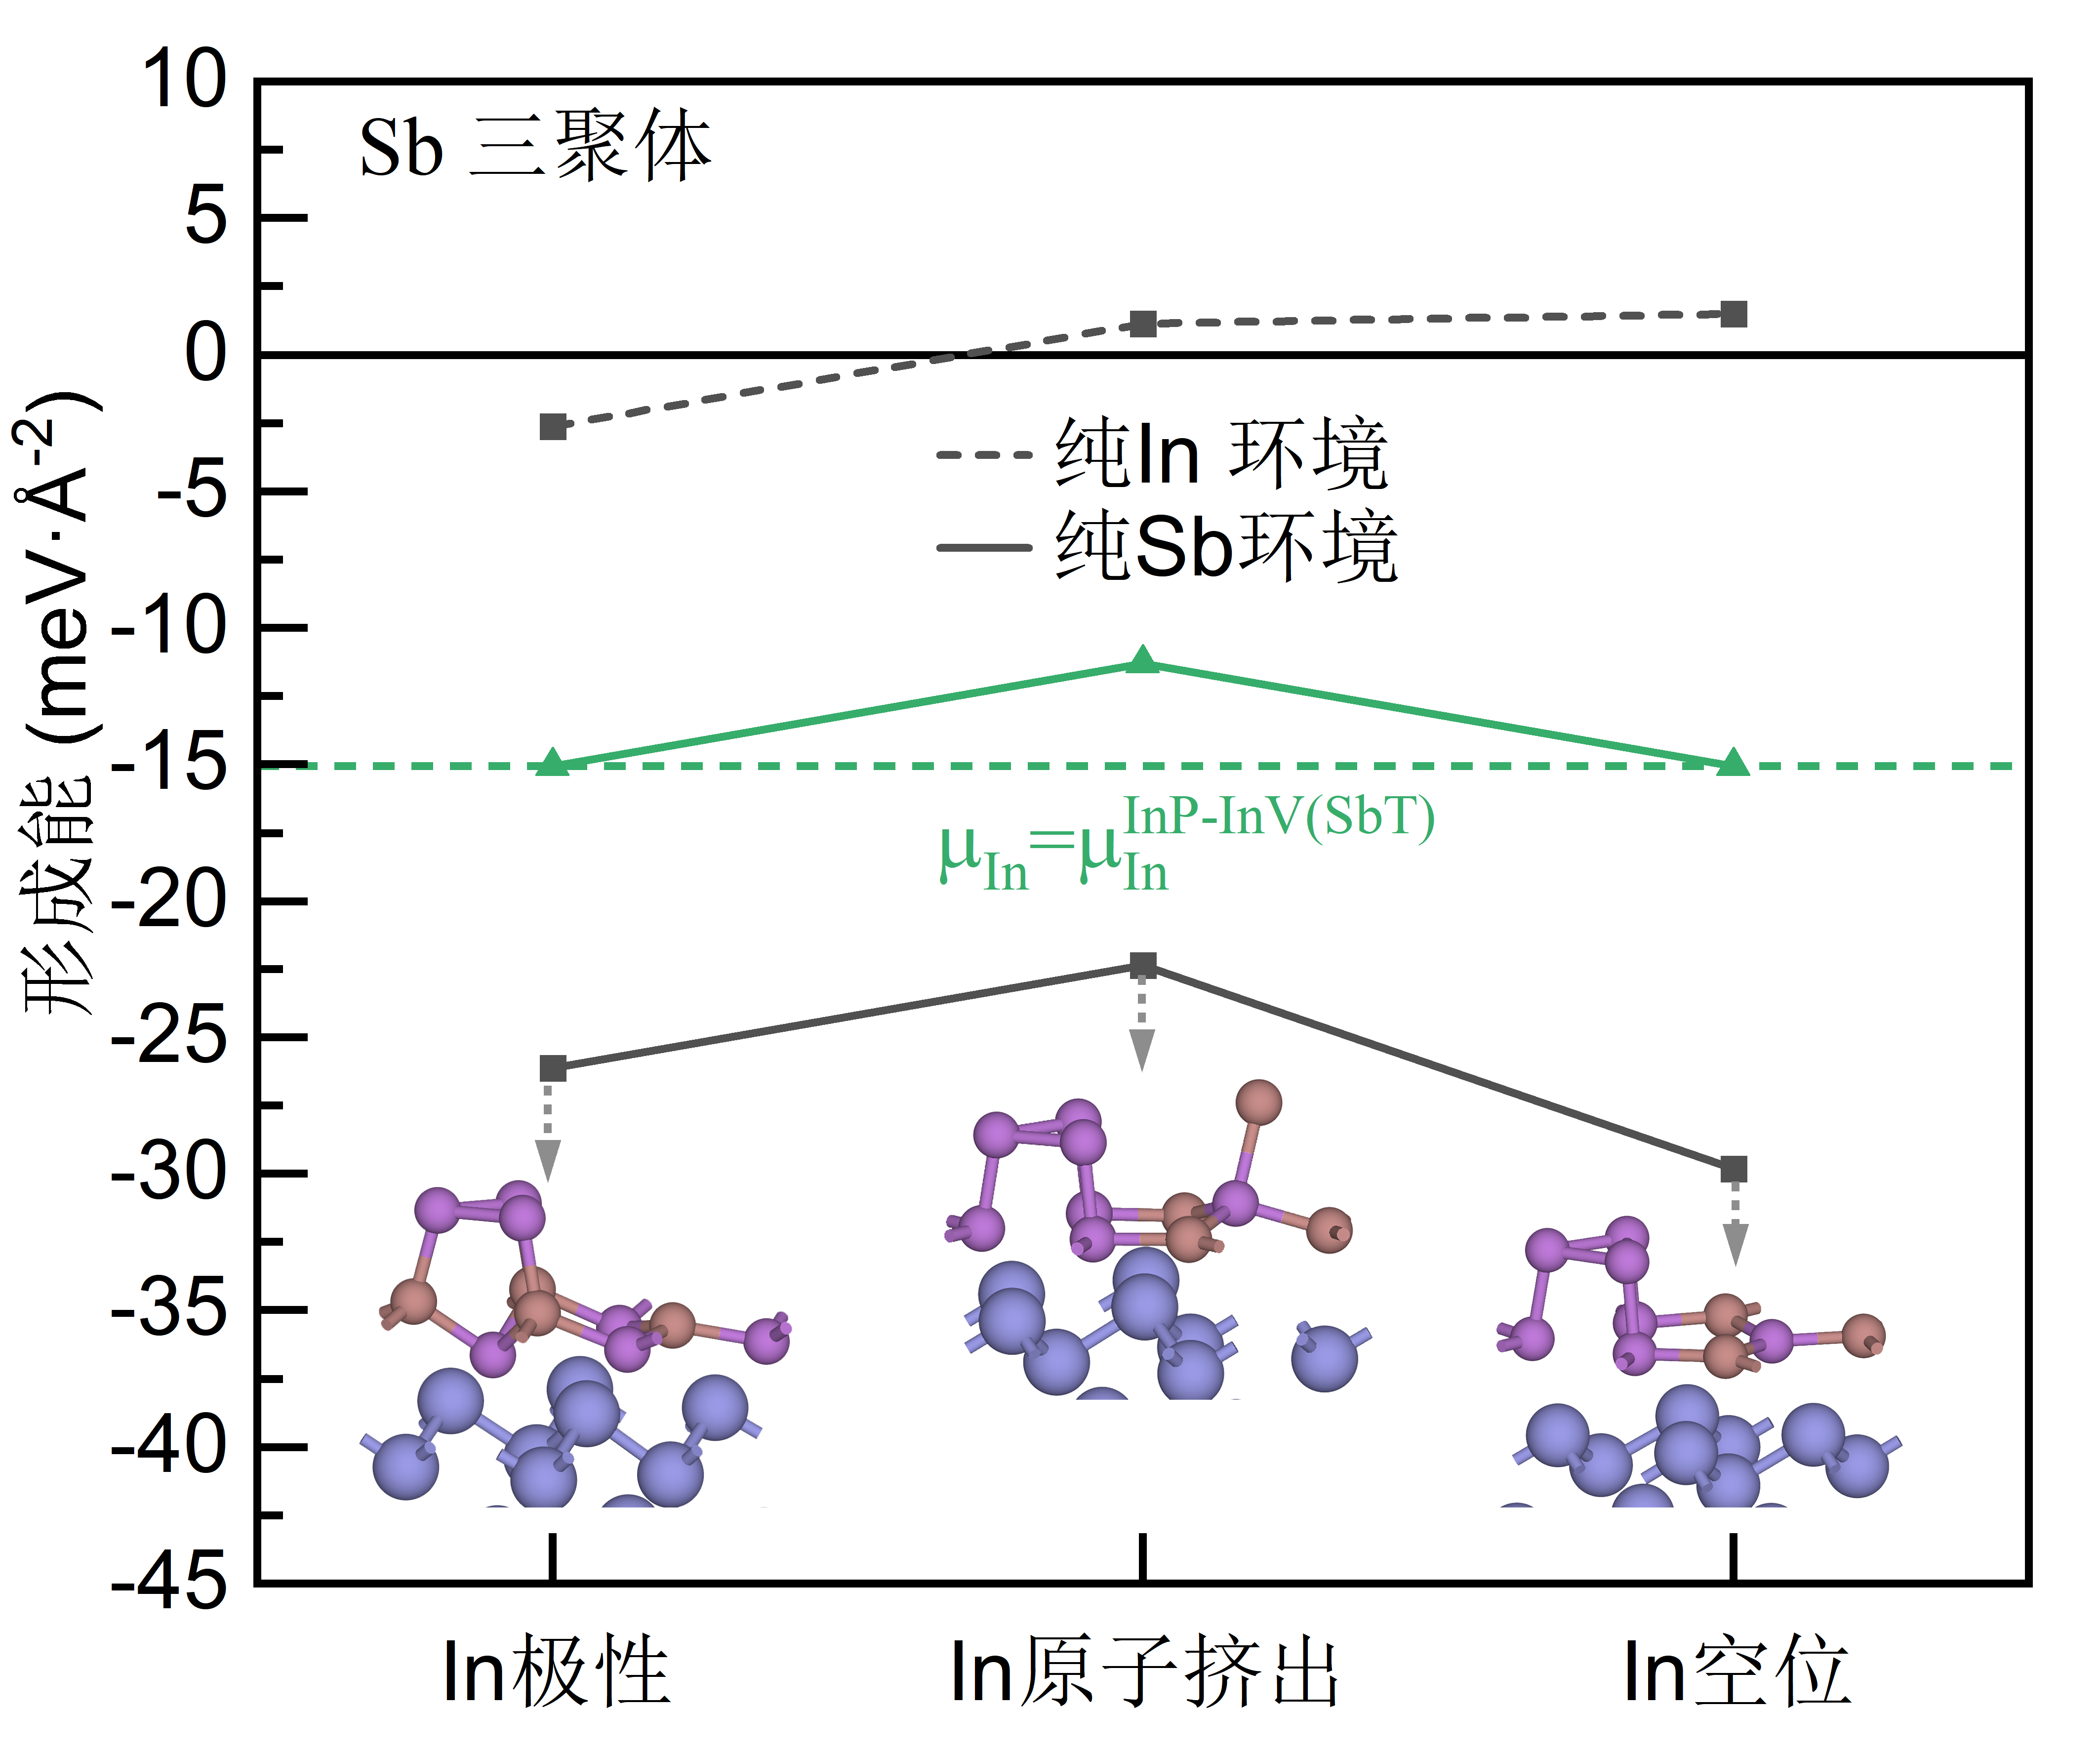
\includegraphics{pic/IS_DFT_2InSb_InPtoInV.png}
    \caption{\cemb{Sb}三聚体重构为第二层时,第一层\cemb{InSb}在\cemb{In}极性和\cemb{In}空位重构构型之间的转换过程。}
    \label{fig:IS_DFT_2InSb_InPtoInV}
\end{figure}

进一步考虑第一层\cemb{InSb}位\cemb{In}空位重构构型的情况,我们在图\ref{fig:IS_2Linsb_InVfirstlayer}中比较了当第二层\cemb{InSb}生长了\cemb{Sb}三聚体重构和\cemb{In}空位层后,第一层位\cemb{In}极性或者\cemb{In}空位层的形成能情况。对于以\cemb{Sb}三聚体重构作为第二层的双层\cemb{InSb},\cemb{In}极性第一层和\cemb{In}空位重构第一层的形成能非常接近。由于\cemb{In}空位重构的第一层缺少一个\cemb{In}原子,其在\cemb{Sb}浓度较高的生长环境中相比于\cemb{In}极性的第一层具有更低的形成能。而当生长环境中的\cemb{In}原子浓度升高后,\cemb{In}原子的活性上升,\cemb{In}极性的\cemb{InSb}第一层开始在形成能方面占据优势。在\cemb{Sb}三聚体结构的第二层下,\cemb{In}空位和\cemb{In}极性的第一层\cemb{InSb}的转变化学式$\muVar{In}{}$为$\muVar{In}{InP-InV\left(SbT\right)}=\SI{-2.8583}{\electronvolt}$。

而对于以\cemb{In}空位重构作为第二层的双层\cemb{InSb},我们可以发现在我们所考虑的$\muVar{In}{}$范围内,以\cemb{In}重构层为第二层比以\cemb{Sb}三聚体重构为第二层的双层\cemb{InSb}具有更低的形成能。同时,以\cemb{In}空位重构作为第一层\cemb{InSb}构型的形成能在最有优势的纯\cemb{Sb}极限环境下仍然不及\cemb{In}极性的构型稳定。因此,当双层\cemb{InSb}在生长的过程中,第二层的\cemb{InSb}由团簇阶段的三聚体生长为\cemb{In}空位重构层时,第一层的\cemb{In}空位构型会在第二层\cemb{In}空位重构层的作用下还原为\cemb{In}极性的构型。

考虑到第一层以混合极性为主的非静态\cemb{InSb}只能在\cemb{Sb}三聚体重构第二层的作用下转变为以\cemb{Sb}极性和\cemb{In}极性为主的多晶态双层\cemb{InSb}。同时在$\muVar{In}{}$的影响下,还会有部分第一层\cemb{InSb}会从\cemb{In}极性转变为以\cemb{In}空位重构的构型。而当更多的原子从生长气氛中沉积到单层\cemb{InSb}的表面,第二层\cemb{InSb}的生长阶段由以\cemb{Sb}三聚体为主的团簇阶段变为\cemb{In}空位表面重构阶段,不仅双层\cemb{InSb}的形成能得到了进一步的降低,第一层中\cemb{Sb}极性的表面也会在\cemb{In}空位表面重构的作用下进一步极化至\cemb{In}极性的构型,同时第一层中\cemb{In}空位也会在体系能量最低的作用下的被还原为\cemb{In}极性。

\begin{figure}[!htb]
    \subfloat[]{
        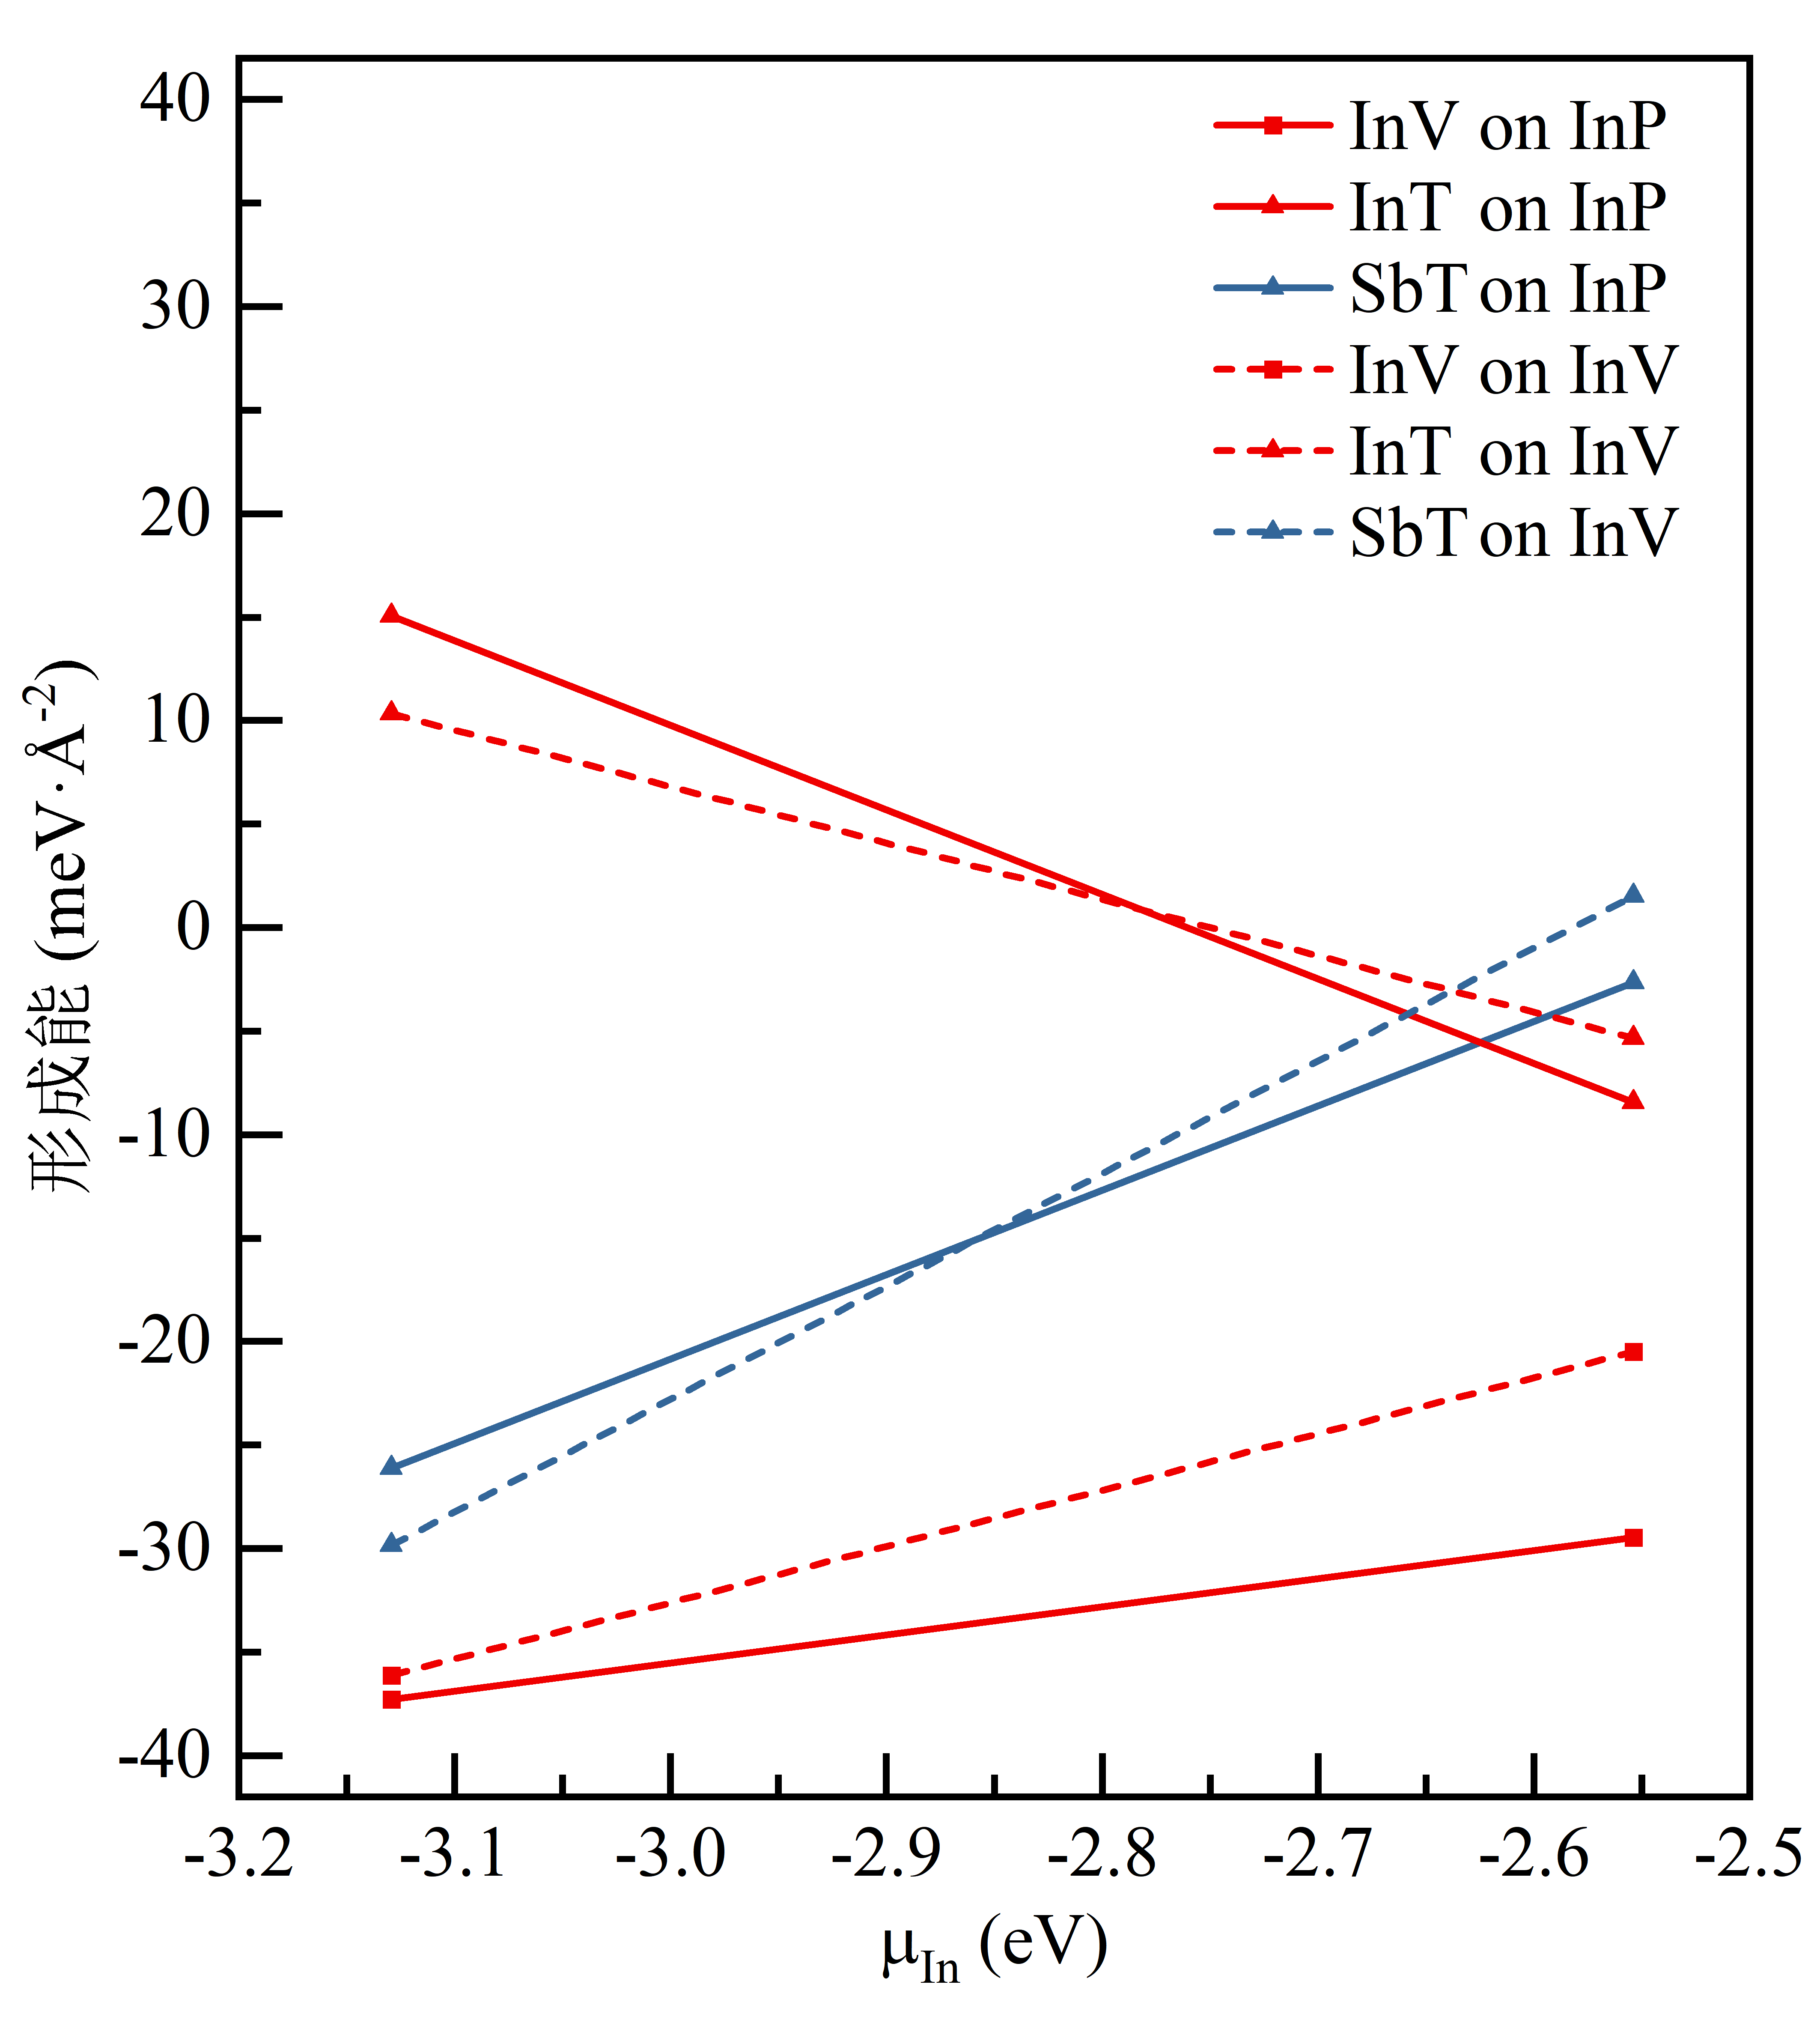
\includegraphics{pic/IS_DFT_2LInSb_SbT-InV-InT_InV-InP.png}
    }\hspace{-5mm}
    \begin{minipage}[b]{0.4\textwidth}
        \subfloat[]{
            \label{fig:IS_structure_SbTonInV}
            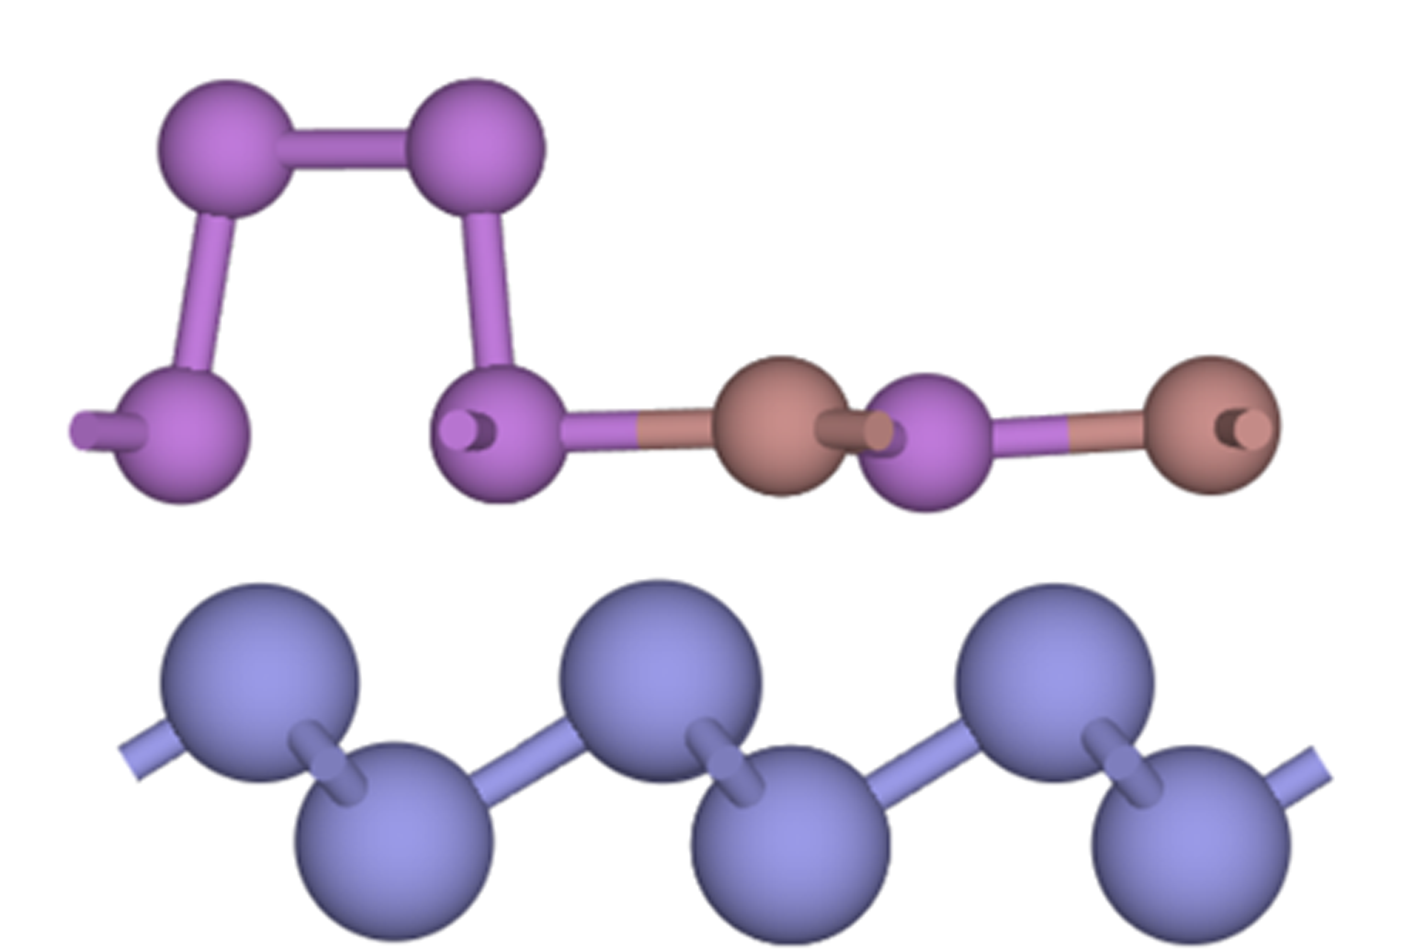
\includegraphics[width=0.9\textwidth]{pic/IS_structure_SbTonInV.png}
        }
        \newline
        \subfloat[]{
            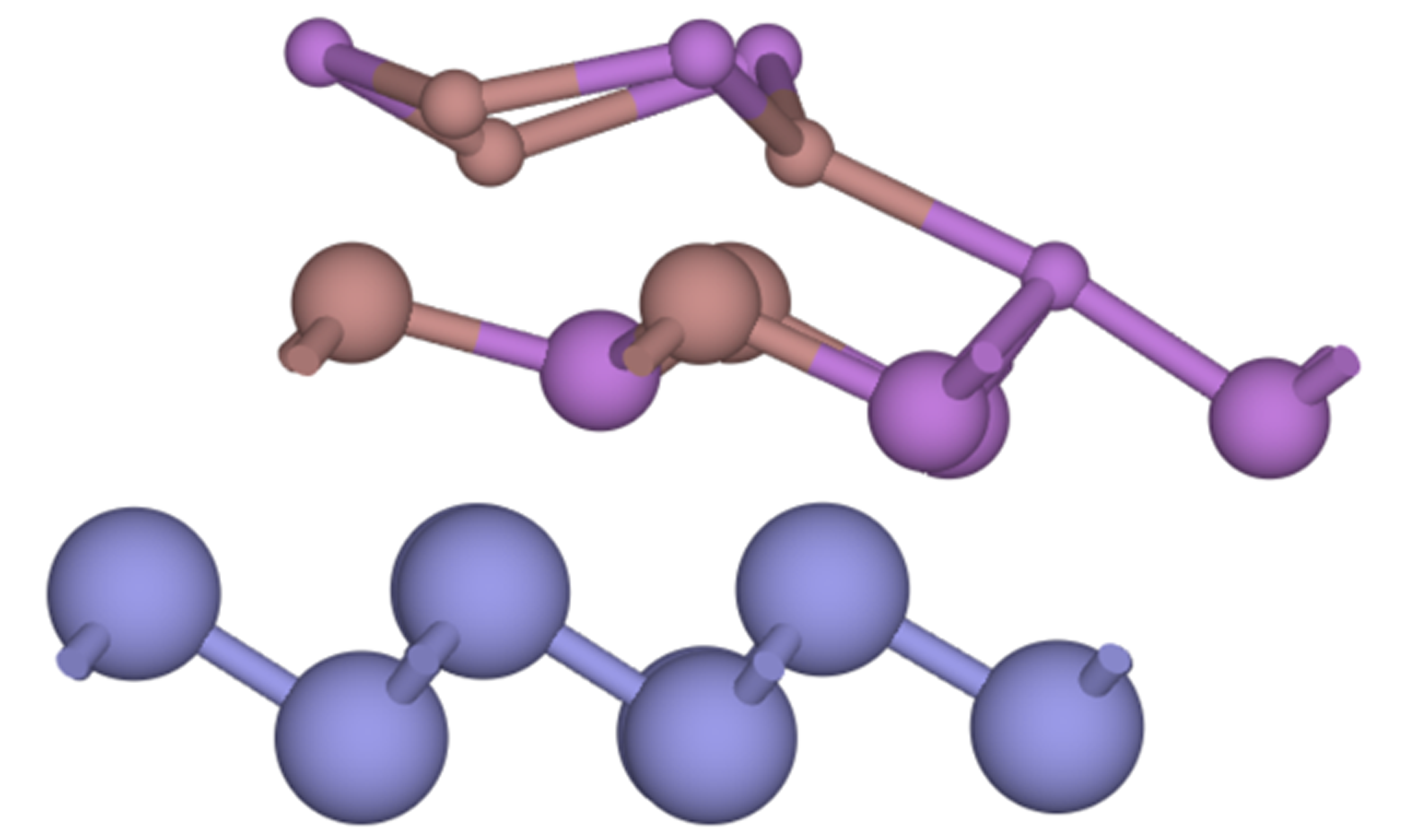
\includegraphics[width=0.9\textwidth]{pic/IS_structure_InVonInV.png}
        }
    \end{minipage}
    \caption{\cemb{Sb}三聚体层和\cemb{In}重构层在\cemb{In}极性和\cemb{In}空位层生长的形成能以及原子结构图。(a)形成能随$\muVar{In}{}$的变化情况;(b)\cemb{Sb}三聚体层\cemb{In}空位\cemb{InSb}上生长的结构图;(c)\cemb{In}空位层\cemb{In}空位\cemb{InSb}上生长的结构图。}
    \label{fig:IS_2Linsb_InVfirstlayer}
\end{figure}

我们将\cemb{InSb}第二层从原子吸附到形成\cemb{In}空位表面重构层的生长序列随着生长环境\cemb{$\muVar{In}{}$}的变化绘制成了生长阶段相图(图\ref{fig:IS_DFT_stagePhase})。在原子吸附阶段,由于在$\InSbMLpolar{2}{2}$ 条形单层\cemb{InSb}表面存在\cemb{Sb}原子和\cemb{In}原子都无法吸附的$\muVar{In}{}$区间(原子脱附区,相图中使用灰色表示)。在这个区间内,由于单层\cemb{InSb}表面原子的缺乏,在第二层\cemb{InSb}生长进入团簇的阶段无法直接形成形成\cemb{In_xSb_{3-x}}团簇。只有当一定数量的\cemb{Sb}原子在热涨落的作用下在\cemb{InSb}的表面聚集,克服表面原子脱附的趋势后才能形成\cemb{Sb}团簇降低形成能。

当环境中的$\muVar{In}{}$位于\cemb{Sb}原子的吸附区间时,生长环境中的\cemb{Sb}原子在混合极性的\cemb{InSb}单层表面沉积,形成\cemb{Sb}三聚体团簇并将第一层的\cemb{InSb}结构引导至\cemb{Sb}极性或者\cemb{In}极性。更低的$\muVar{In}{}$(更加接近纯\cemb{Sb}极限环境)还可能使第一层中的某些\cemb{In}原子脱离,在第一层\cemb{InSb}中形成\cemb{In}缺陷($\muVar{In}{}\leqslant \muVar{In}{InP-InV\left(SbT\right)}$)。

在$\muVar{In}{}$取值的另一边,\cemb{In}原子吸附区的开端,由于缺乏\cemb{Sb}原子,无法在单层的\cemb{InSb}直接形成\cemb{Sb}三聚体团簇。生长环境中的\cemb{Sb}原子只能借助已吸附的\cemb{In}原子,形成\cemb{In1Sb2}团簇作为中间态。经过进一步的结构演化后,\cemb{In1Sb2}团簇中的\cemb{In}原子被环境中的\cemb{Sb}原子替代,形成更加稳定的\cemb{Sb}三聚体团簇。当$\muVar{In}{}$的取值更加接近纯\cemb{In}极限环境时,在\cemb{In}极性表面形成\cemb{Sb}三聚体的形成能会高于在\cemb{In}空位重构的第一层表面形成\cemb{In3Sb1}团簇的能量。在这种情况下,第二层\cemb{InSb}以\cemb{In3Sb1}团簇的形式存在,并且会将第一层\cemb{InSb}的结构转化成类似于\cemb{In}空位重构的构型。

随着生长的继续进行,更多环境中的\cemb{In}原子和\cemb{Sb}原子参与到第二层\cemb{InSb}的生长之中,使得第二层\cemb{InSb}的结构向\cemb{In}空位表面重构转化。\cemb{In}空位表面重构在第二层\cemb{InSb}的形成同时也驱使第一层\cemb{InSb}的构型转变为统一的\cemb{In}极性,完成双层\cemb{InSb}的自极化过程。

\begin{figure}[!htb]
    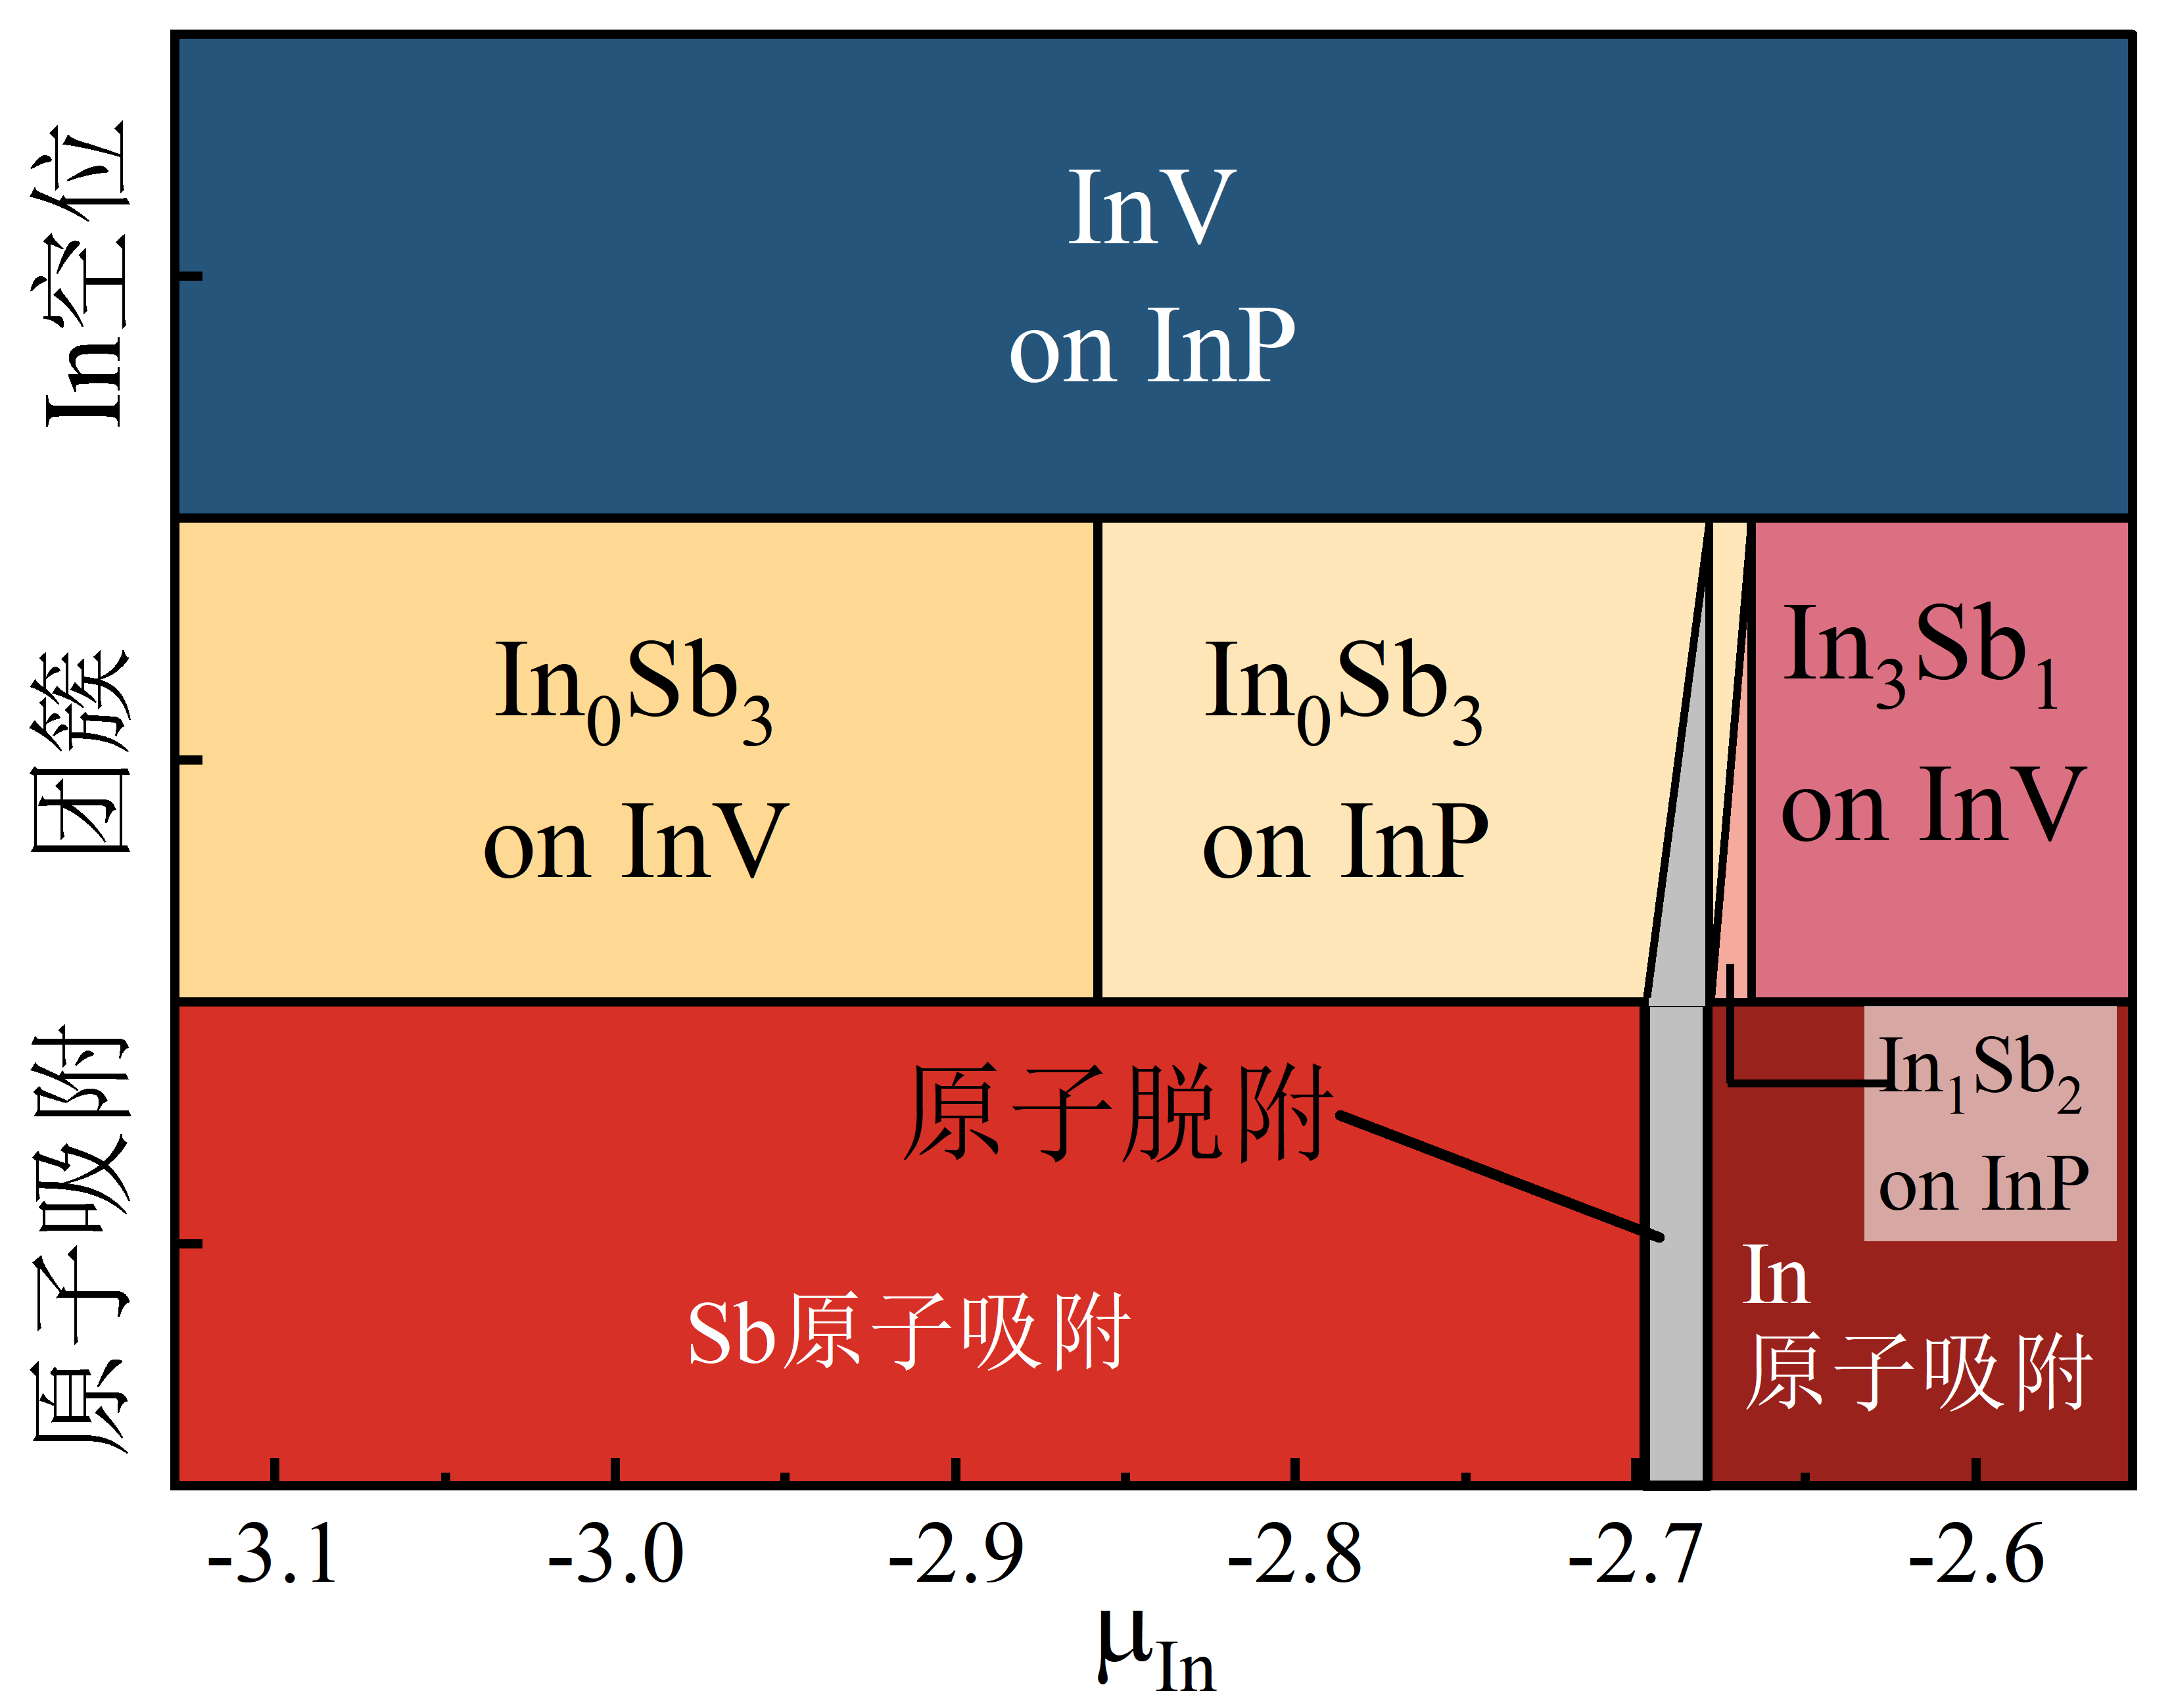
\includegraphics{pic/IS_DFT_stagePhase.png}
    \caption{双层\cemb{InSb}不同生长阶段的自极化相图。}
    \label{fig:IS_DFT_stagePhase}
\end{figure}

\subsection{双层锑化铟的极性演化}

在上一章中,我们对于双层\cemb{InSb}生长的极化过程的研究集中在第二层\cemb{InSb}的覆盖率为1的情况。在本章中,通过引入不同覆盖度的第二层\cemb{InSb},我们可以进一步探究\cemb{InSb}极化过程和沉积时间之间的关系。在本章中,我们将双层\cemb{InSb}的极化过程分为三个阶段\chinesecolon 第一个阶段为非晶态阶段(无第二层);第二个阶段为多晶阶段(第二层为\cemb{Sb}三聚体重构);第三个阶段为\cemb{In}极性阶段(第二层为\cemb{In}空位重构)。对于第一层的\cemb{InSb},我们选用$\InSbMLpolar{2}{2}$ 条形构型和\cemb{In}极性($\InSbMLpolar{4}{0}$)构型来表示非极化的和在第二层\cemb{InSb}作用下极化的第一层\cemb{InSb}。对于沉积时间,我们假设生长环境中的原子在单层\cemb{InSb}的表面沉积是连续、均匀的。因此我们使用在单层\cemb{InSb}表面沉积、形成第二层\cemb{InSb}的吸附原子数量$\NumOfAdatom$来代表第二层\cemb{InSb}的沉积生长时间。同时,为了对具有不同覆盖度不同覆盖度的第二层的双层\cemb{InSb}进行计算,如图\ref{fig:IS_diagram_2Linsb_partial}所示,我们将模拟原胞扩大到$4 \times 4$\cemb{InSb}切片模型,并将整个\cemb{InSb}单层区域的表面分成四个独立的第二层\cemb{InSb}生长区块,可以提供以$1/ 4$覆盖率为间隔的部分覆盖\cemb{InSb}第二层生长。

\begin{figure}[htb]
    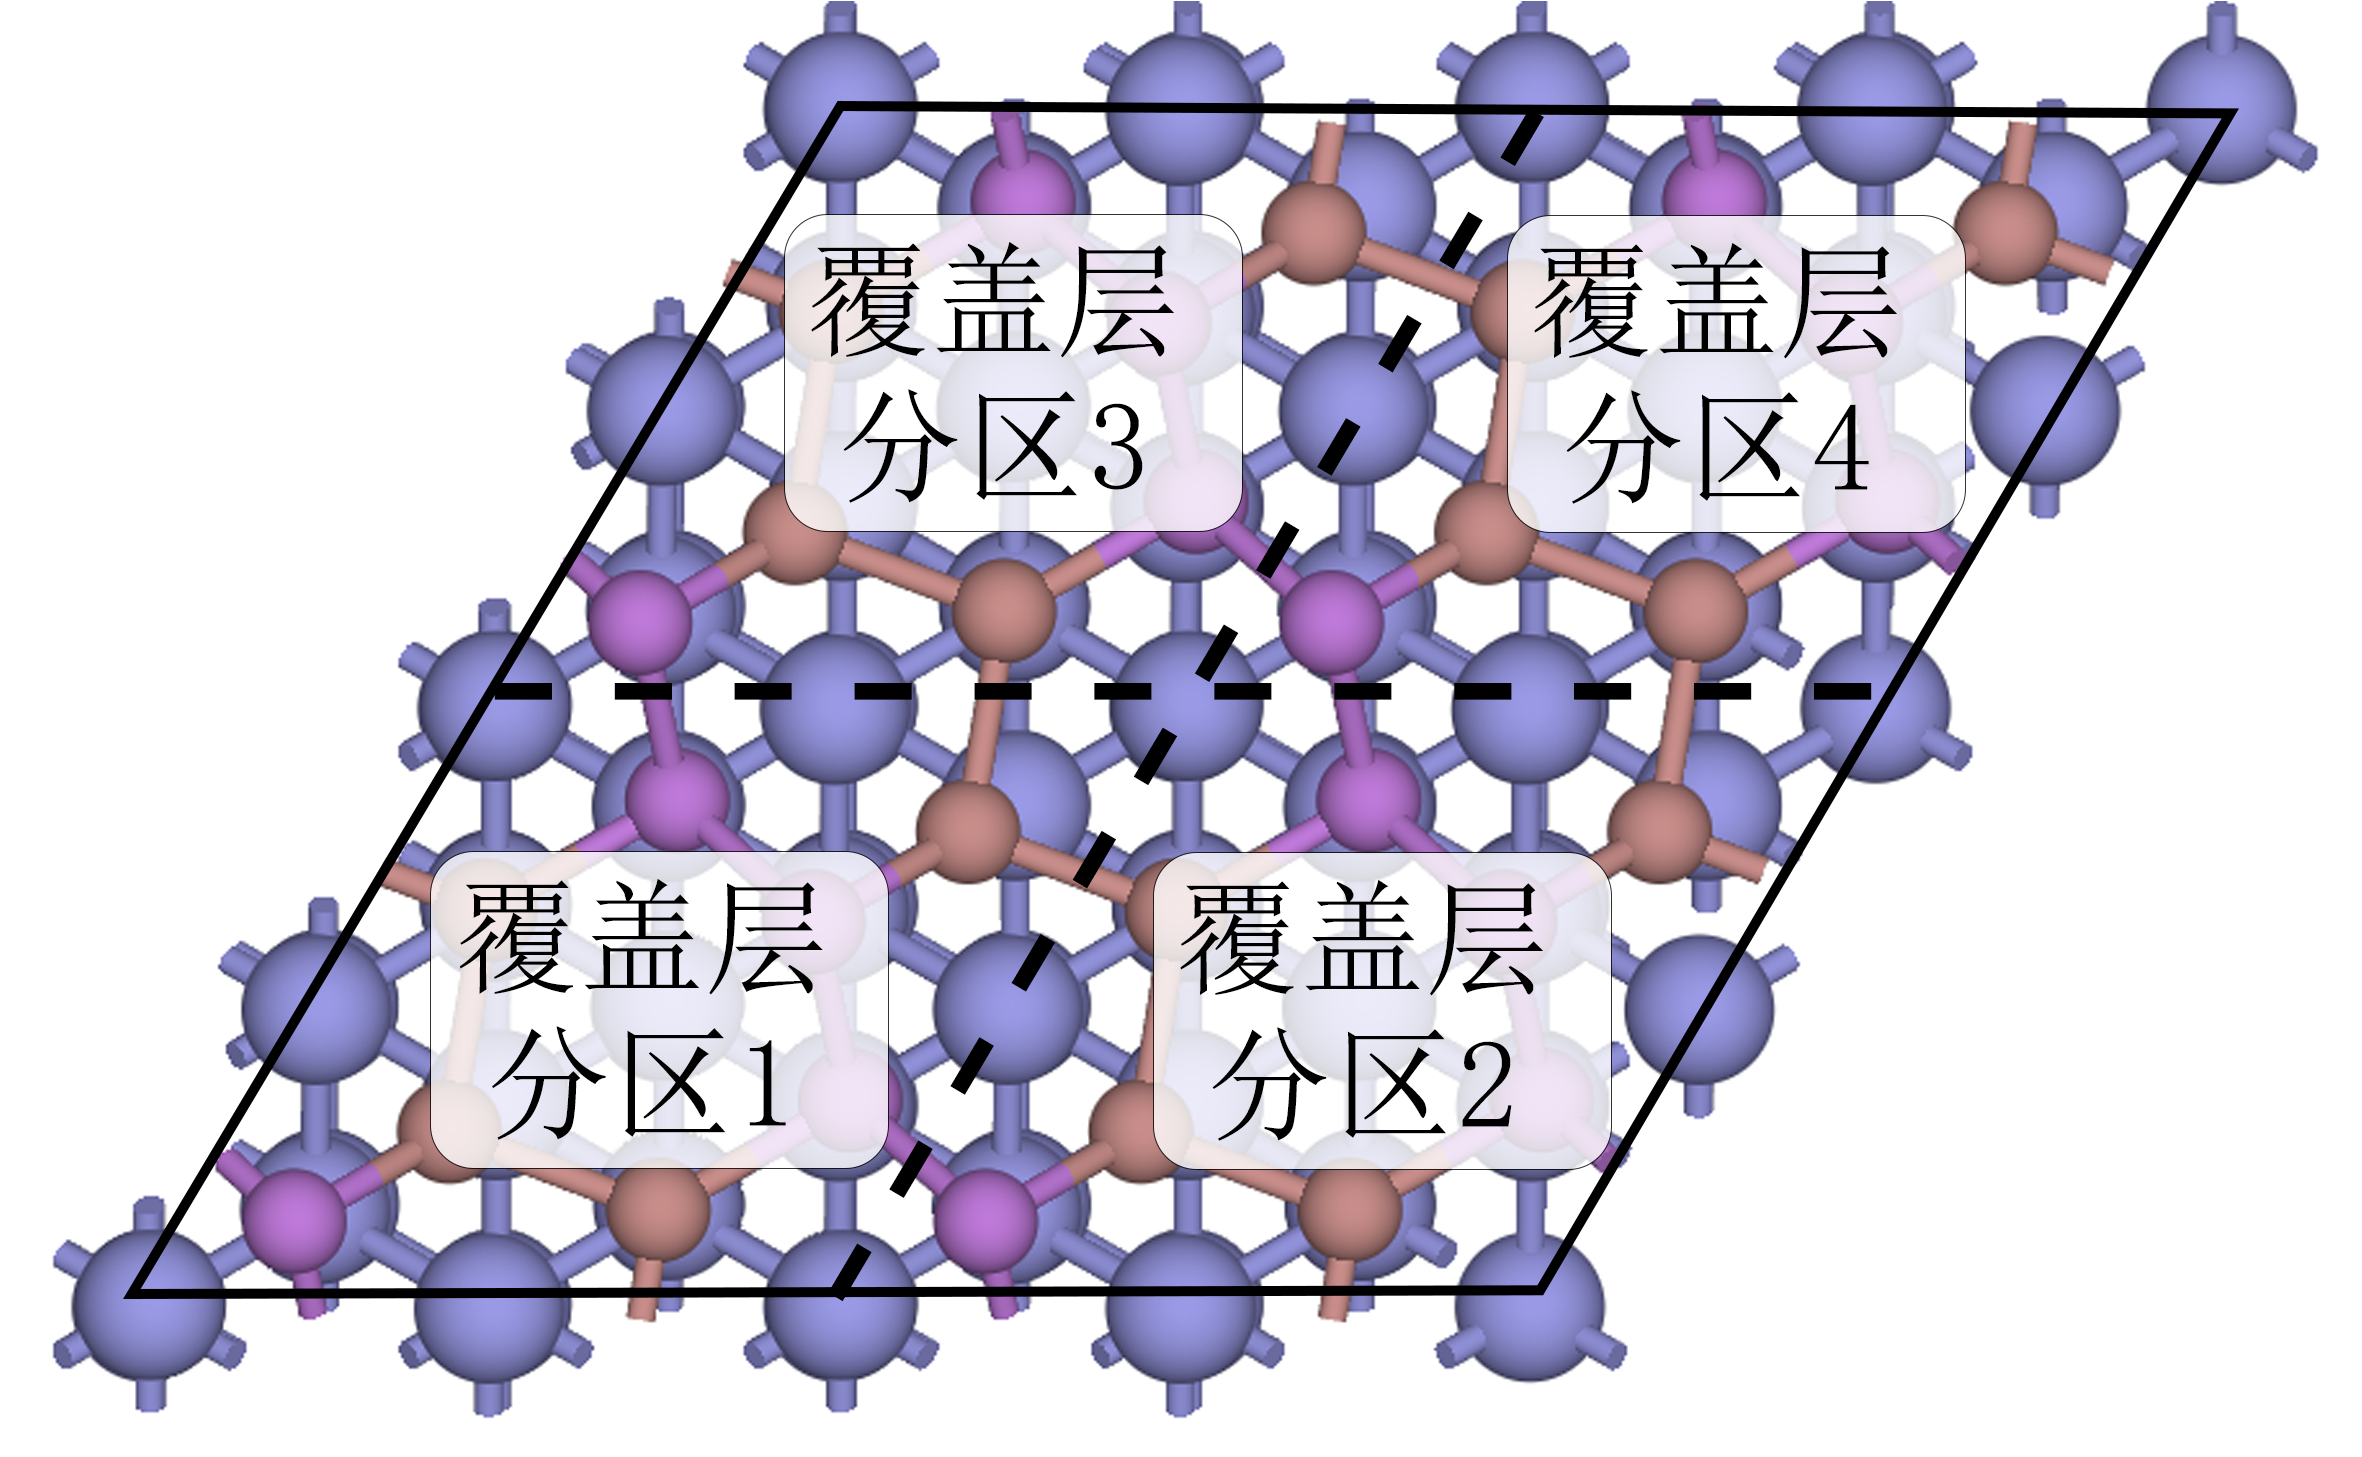
\includegraphics{pic/IS_diagram_2Linsb_partial.png}
    \caption{$4 \times 4$\cemb{InSb}切片模型中四个独立的第二层\cemb{InSb}生长区块示意图。}
    \label{fig:IS_diagram_2Linsb_partial}
\end{figure}

对于双层\cemb{InSb}的生长,在本章中我们将关注重点放在第二层为\cemb{Sb}三聚体表面重构构型和\cemb{In}空位表面重构对于第一层\cemb{InSb}极性的转化过程。为了减小搜索范围,当第二层为\cemb{Sb}三聚体重构时,第一层\cemb{InSb}中\cemb{In}空位的形成仅通过$\muVar{In}{}$与转变点$\muVar{In}{InP-InV\left(SbT\right)}$的关系进行判定。

我们使用$C^{N_{\rm InV}\rm InV}_{N_{\rm SbT}\rm SbT}$来表示部分二层生长的双层\cemb{InSb}的原子构型。其中$C$是已生长的第二层\cemb{InSb}的总覆盖度,$N_{\rm InV}$和$N_{\rm SbT}$代表\cemb{In}空位重构和\cemb{Sb}三聚体重构在模拟晶胞中占据的区块的数量。

在图\ref{fig:IS_DFT_2LInSb_partEnergy}中,我们绘制了在纯\cemb{Sb}和纯\cemb{In}极限的生长环境下双层\cemb{InSb}随着沉积时间增长的形成能分布和极性演化过程。在纯\cemb{Sb}环境中,\cemb{Sb}三聚体表面重构拥有非常高的形成能能量优势。随着沉积原子数的上升,越来越多的\cemb{Sb}三聚体表面重构在单层\cemb{InSb}的表面生长,并且将各自下方区域的第一层\cemb{InSb}局部得转变为\cemb{In}极性或者\cemb{Sb}极性的结构。第一层\cemb{InSb}的首次极化开始于$\CNinNsb{3}{4}{0}{3}$。在$\CNinNsb{3}{4}{0}{3}$构型的双层\cemb{InSb}中,最后一块未生长第二层\cemb{InSb}的区块在边界能的作用下自发转变成与周围相同极化的晶态结构,使得整个双层\cemb{InSb}在覆盖度为$\frac{3}{4}$的\cemb{Sb}三聚体第二层的作用下被极化为以\cemb{In}极性和\cemb{Sb}极性为主的多晶构型。在纯\cemb{Sb}极限环境中高活性的\cemb{Sb}原子不仅促进了\cemb{Sb}三聚体重构第二层的生长,而且还阻止了以\cemb{In}空位重构为构型的第二层的形成。根据我们的形成能计算,包含6个吸附原子的$\CNinNsb{1}{2}{0}{2}$构型的形成能低于包含7个吸附原子的$\CNinNsb{1}{4}{1}{0}$。因此在生长了覆盖率为$\frac{1}{2}$的\cemb{Sb}三聚体重构第二层后,生长气氛中的\cemb{In}原子和\cemb{Sb}原子并不会在已经形成的\cemb{Sb}三聚体团簇的基础上继续生长出\cemb{In}空位重构,而是直接在未生长第二层的表面生长\cemb{Sb}三聚体重构第二层,从而形成能量更低的$\CNinNsb{3}{4}{0}{3}$构型的双层\cemb{InSb}。同时,包含9个吸附原子的$\CNinNsb{3}{4}{0}{3}$构型的形成能也低于包含10个吸附原子的$\CNinNsb{1}{2}{1}{1}$构型。因此在生长了覆盖率$\frac{1}{3}$的\cemb{Sb}三聚体重构的第二层后,\cemb{In}空位第二层同样无法在三聚体重构的基础上生成。知道生长了满覆盖的\cemb{Sb}三聚体重构后,包含12个吸附原子的$\CNinNsb{1}{1}{0}{4}$的形成能低于包含13个吸附原子的$\CNinNsb{3}{4}{1}{2}$、包含14个吸附原子的$\CNinNsb{1}{2}{2}{0}$、包含16个吸附原子的$\CNinNsb{1}{1}{1}{3}$、包含17个吸附原子的$\CNinNsb{3}{4}{2}{1}$。在跳过了这四个构型后,在纯\cemb{Sb}极限环境下的$\CNinNsb{1}{1}{0}{4}$构型倾向于直接生成更加稳定的$\CNinNsb{1}{1}{2}{2}$,包含20个吸附原子。$\CNinNsb{1}{1}{2}{2}$构型的形成同时在\cemb{In}空位重构的作用下,第一层\cemb{InSb}的被极化为\cemb{In}极性,完成双层\cemb{InSb}的极化过程。继续吸附生长环境中更多的原子可以形成满覆盖的\cemb{In}空位重构第二层,进一步降低\cemb{In}极性第二层的形成能,提升极化水平。

\begin{figure}
    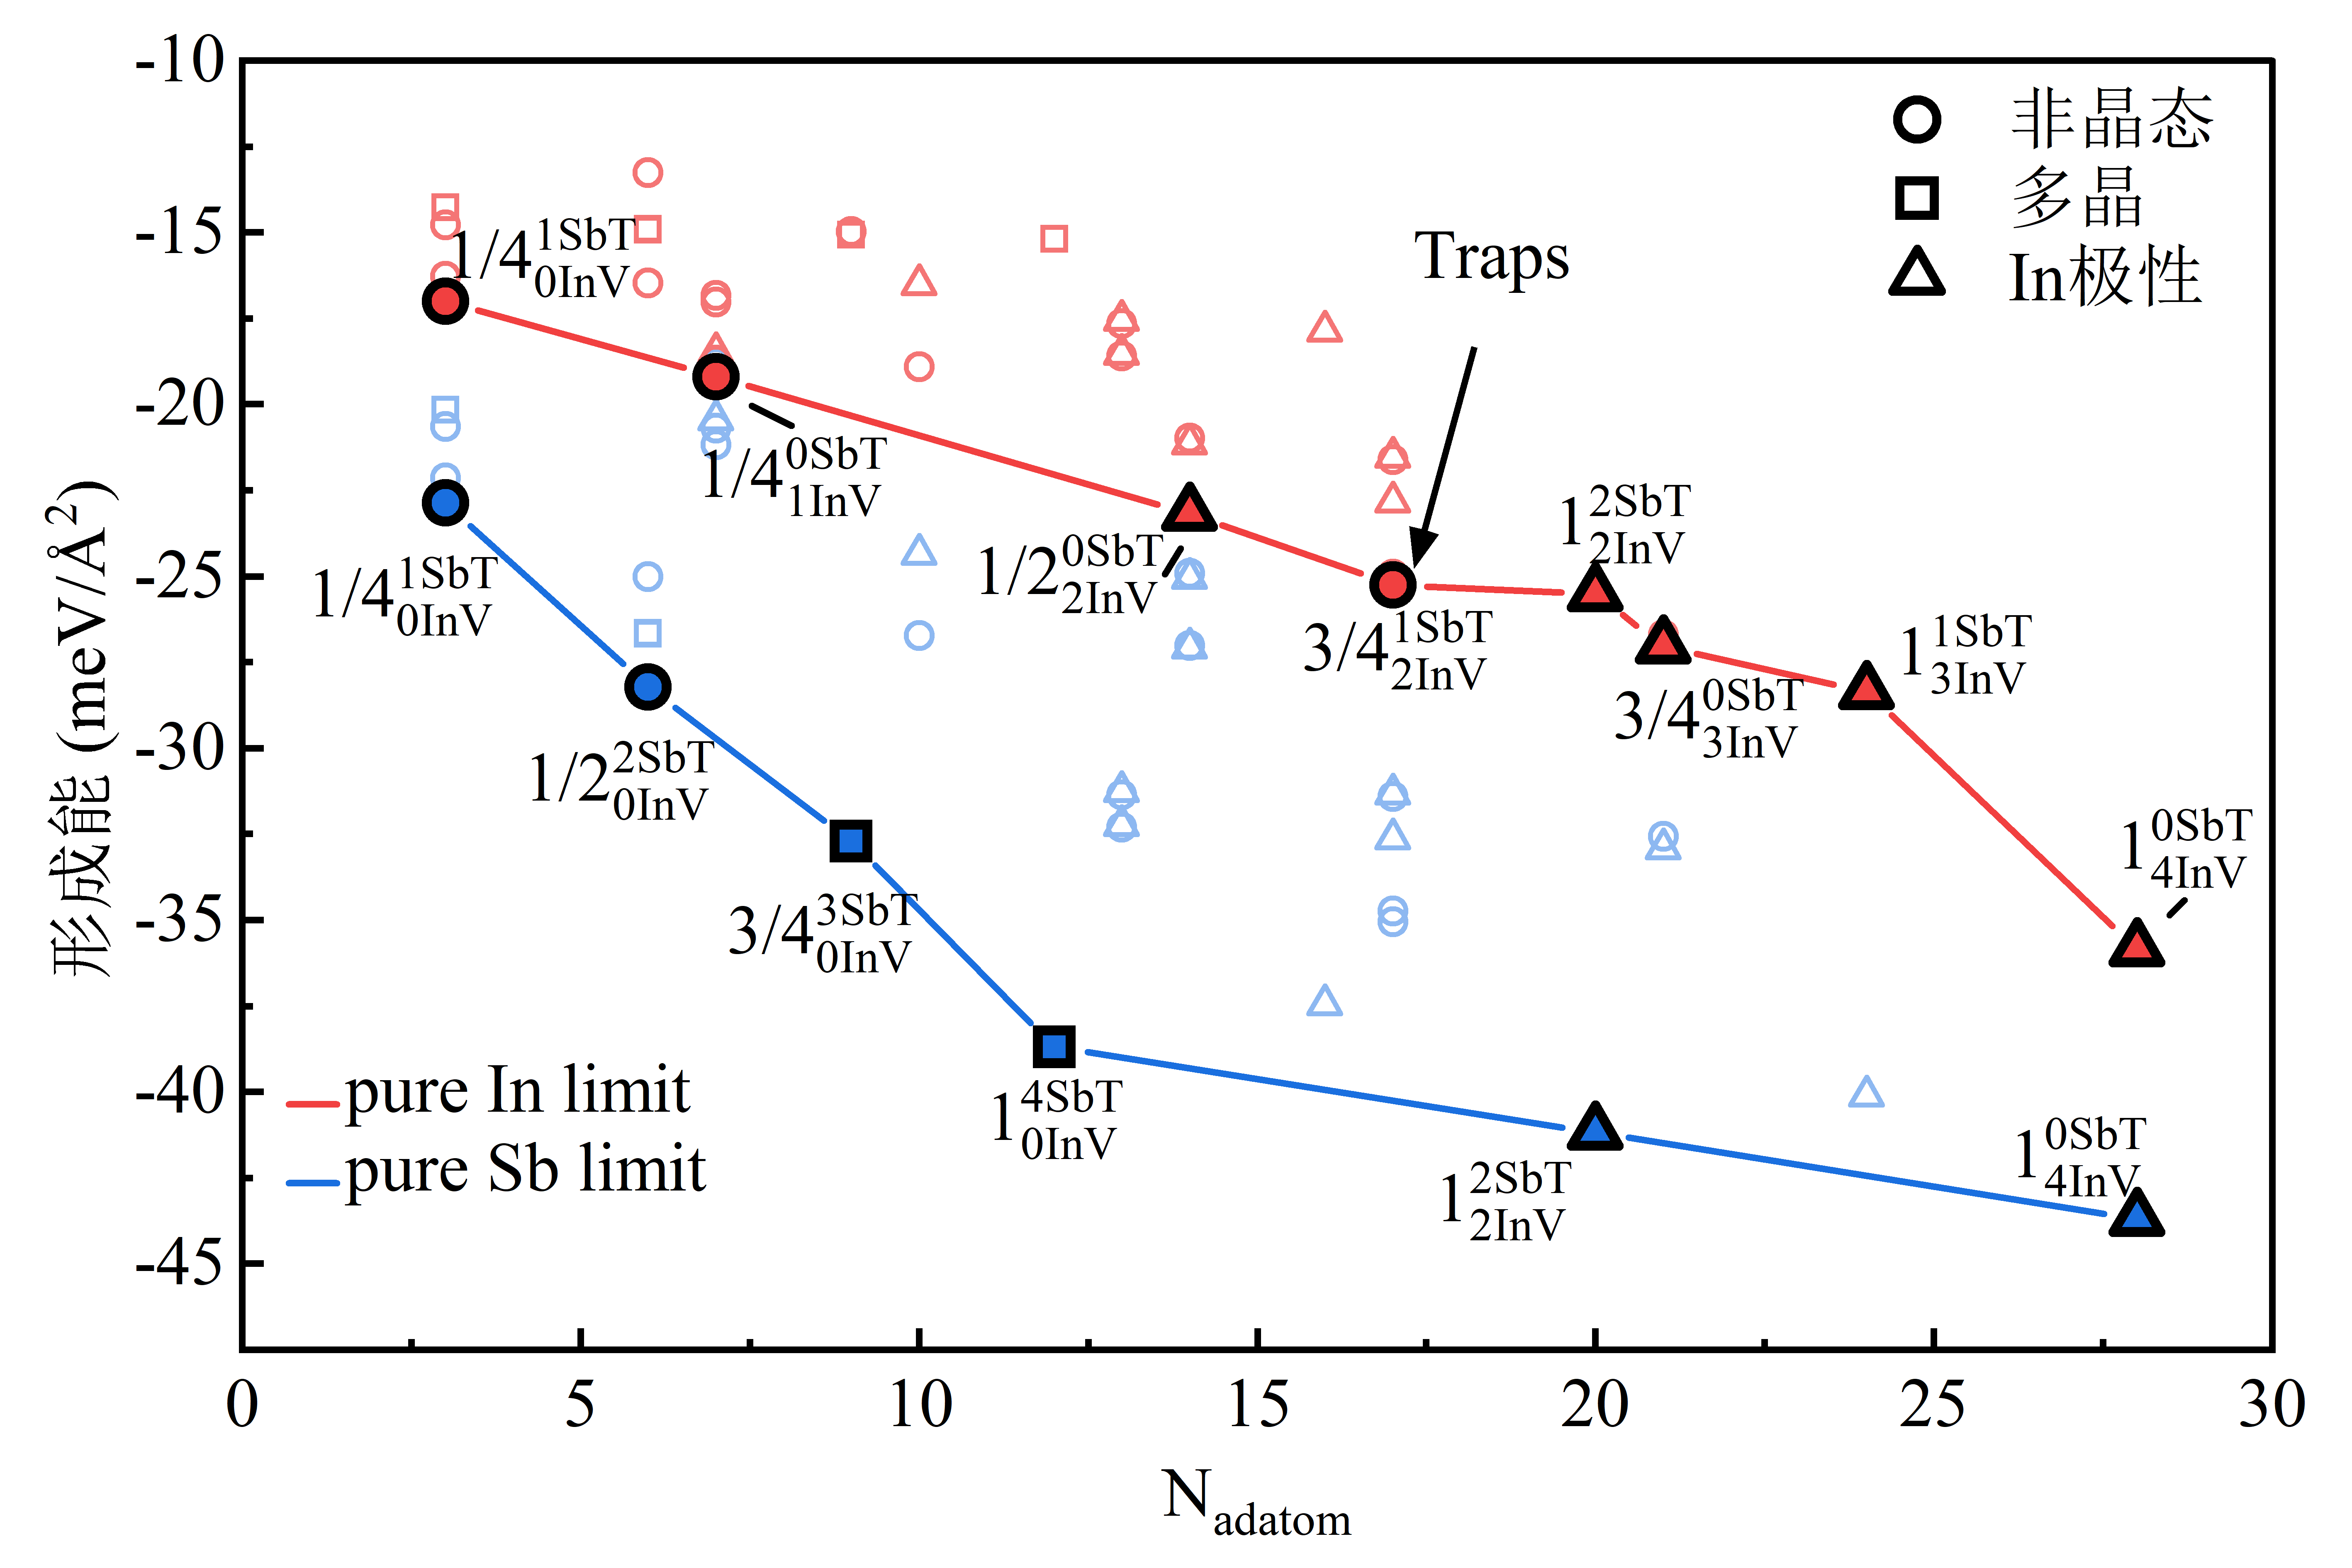
\includegraphics{pic/IS_DFT_2LInSb_partEnergy.png}
    \caption{不同生长环境下双层\cemb{InSb}随着沉积时间增长的形成能分布和极性演化过程。}
    \label{fig:IS_DFT_2LInSb_partEnergy}
\end{figure}


在纯\cemb{In}环境中,环境中的\cemb{Sb}原子很难在单层的\cemb{InSb}表面沉积,同时较高的$\muVar{In}{}$取值也导致形成\cemb{Sb}三聚体重构第二层的形成能较大。在这种情况下,随着生长过程而吸附在单层\cemb{InSb}表面的原子更倾向于直接形成\cemb{In}空位的第二层($\CNinNsb{1}{4}{1}{0}$),同时也将对应区块下的第一次层\cemb{InSb}局域地极化成\cemb{In}极性地构型。在聚集了14个吸附原子后,\cemb{InSb}单层的表面形成了覆盖率为$\frac{1}{2}$的\cemb{In}空位重构第二层。在这个过程中,双层\cemb{InSb}的极化过程直接跳过了多晶的步骤,$\CNinNsb{1}{2}{2}{0}$结构的第二层将未覆盖第二层的区域一并转变为了\cemb{In}极性的构型。在这种情况下,未覆盖第二层的单层\cemb{InSb},由于不同极性之间过高的晶界能,被迫与另邻位的被第二层所极化区域保持同样的极性构造,以保持形成能的最小化。虽然早早得完成了全区域第一层向\cemb{In}极性结构的转变,但在$\CNinNsb{1}{2}{2}{0}$结构的第二层下,全\cemb{In}极性的第一层的形成能仅比包含非晶态的第一层的形成能高\SI{0.07}{\mievpas}。如此小的差距并不能保证双层\cemb{InSb}能够在热动能的影响下继续保持\cemb{In}极性的状态。进一步的计算表明,$\CNinNsb{1}{2}{2}{0}$继续吸附气氛中的三个\cemb{Sb}原子后,会在第二层中形成$\CNinNsb{3}{4}{2}{1}$结构。这个结构的产生不仅破坏了的原本规整的第二层\cemb{InSb}的晶格,而且还会在双层\cemb{InSb}的极化过程中成为一个陷阱步骤。使得原本在$\CNinNsb{1}{2}{2}{0}$结构的第二层下完成极化的\cemb{In}极性双层\cemb{InSb}转变为非晶态的构型。要越过这个$\CNinNsb{3}{4}{2}{1}$导致的陷阱步骤,需要进一步在单层\cemb{InSb}的表面上沉积原子,使得第二层的覆盖率达到1,形成$\CNinNsb{1}{1}{2}{2}$结构。在$\CNinNsb{1}{1}{2}{2}$结构的第二层下,第一层\cemb{InSb}的结构到\cemb{In}极性的状态,但$\CNinNsb{1}{1}{2}{2}$结构下\cemb{In}极性的双层\cemb{InSb}的形成能只比陷阱步$\CNinNsb{3}{4}{2}{1}$结构下非晶态的双层\cemb{InSb}的形成能低\SI{0.27}{\mievpas}。因此只靠形成$\CNinNsb{1}{1}{2}{2}$结构的第二层并不能保证双层\cemb{InSb}的再次完全极化。为了进一步巩固极化的成果,需要吸附生长环境中更多的原子,计算显示\cemb{In}空位重构在第二层的覆盖率越大,\cemb{In}极性的双层\cemb{InSb}的形成能相对于非晶态陷阱步的优势就越大。在$\CNinNsb{1}{1}{4}{0}$结构的第二层下,\cemb{In}极性的双层\cemb{InSb}的形成能比陷阱步$\CNinNsb{3}{4}{2}{1}$结构下非晶态的形成能低大约\SI{10.61}{\mievpas}。

\begin{figure}
    \subfloat[]{
        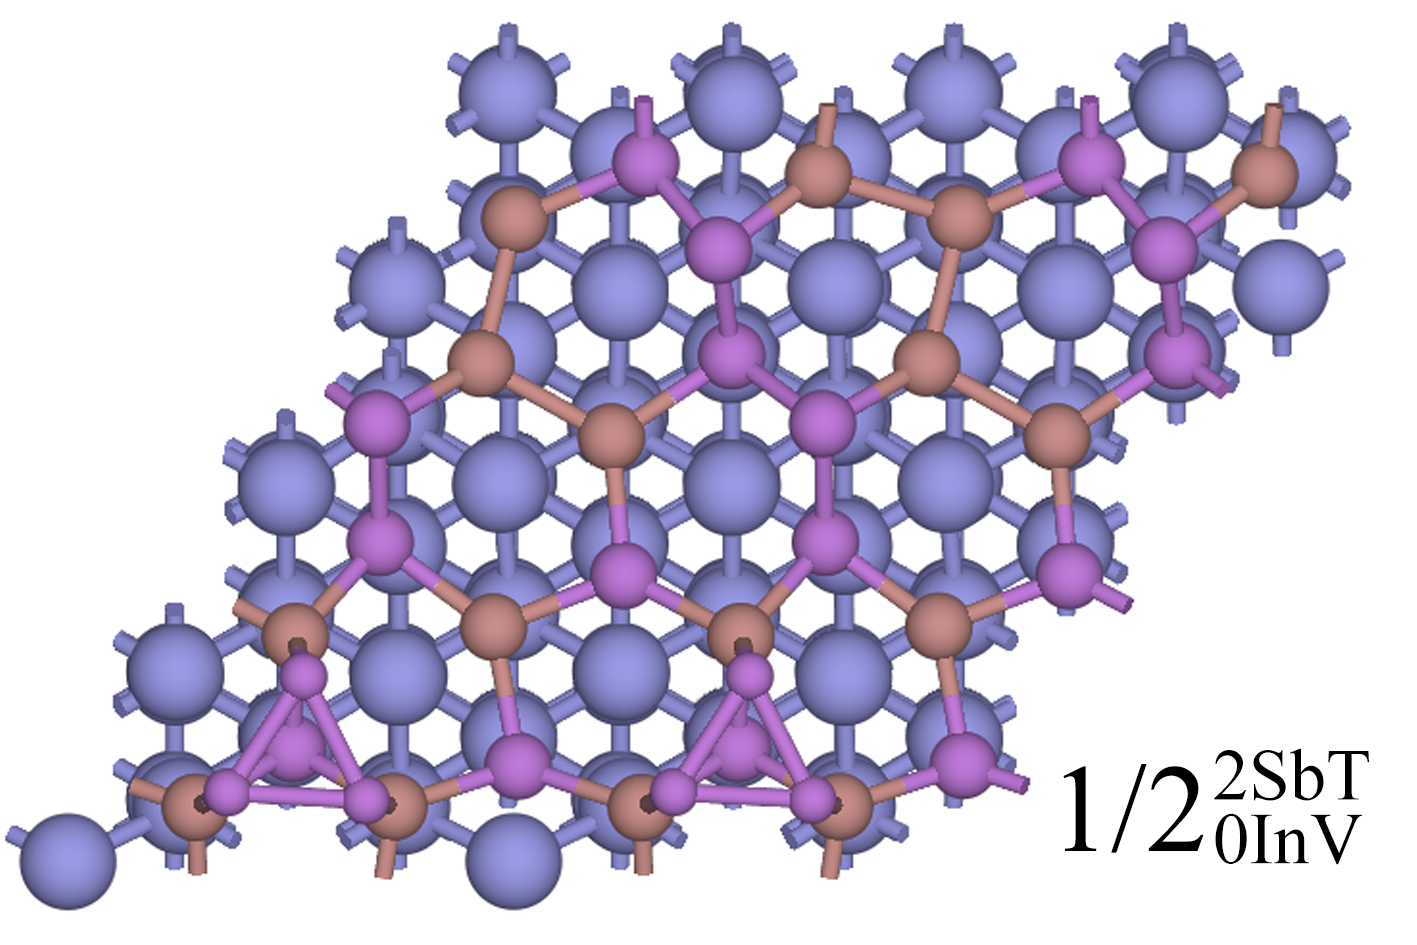
\includegraphics{pic/IS_structure_partical_1-2_0-2.png}
    }
    \subfloat[]{
        \includegraphics{pic/IS_structure_partical_1-2_2-0.png}
    }\\[-1ex]
    \subfloat[]{
        \includegraphics{pic/IS_structure_partical_3-4_2-1.png}
    }
    \subfloat[]{
        \includegraphics{pic/IS_structure_partical_3-4_0-3.png}
    }
\end{figure}

对于极化陷阱步$\CNinNsb{3}{4}{2}{1}$结构的形成,我们在这里从原子结构的角度进行简单分析。
%//TODO continue here

\begin{figure}
    \includegraphics{pic/IS_DFT_2LInSb_partPhase.png}
\end{figure}
\subsection{双层锑化铟的极性演化机理}
\subsubsection{赝氢饱和法和四面体法计算不同\cemb{InSb}表面的表面形成能}
在赝氢饱和法中,具有 %//TODO

在四面体法中,%//TODO
\begin{figure}
    \subfloat[]{
        \includegraphics{pic/IS_structure_slab_pseH_SbT.png}
    }\\[-0.5ex]
    \subfloat[]{
        \includegraphics{pic/IS_structure_slab_pseH_InP.png}
    }
\end{figure}

\begin{figure}
    \subfloat[]{
        \includegraphics[width=0.45\textwidth]{pic/IS_structure_cluster_2.png}
    }
    \subfloat[]{
        \includegraphics[width=0.45\textwidth]{pic/IS_structure_cluster_3.png}
    }\\[-0.5ex]
    \subfloat[]{
        \includegraphics[width=0.45\textwidth]{pic/IS_structure_cluster_7.png}
    }
    \subfloat[]{
        \includegraphics[width=0.45\textwidth]{pic/IS_structure_cluster_8.png}
    }
\end{figure}

\subsubsection{表面能驱动的双层锑化铟的极性演化机理}

\begin{figure}
    \includegraphics{pic/IS_DFT_surfaceE_InPSbP.png}
\end{figure}

\begin{figure}
    \includegraphics{pic/IS_DFT_PDOS-COHP.png}
\end{figure}

\begin{figure}
    \includegraphics{pic/IS_DFT_surfaceE_InVSbT.png}
\end{figure}
\section{总结}